% New-submission version of the study (journal not yet chosen; IEEEtran is a
% neutral working format).  Every result number is a macro: primary analysis
% in generated/numbers.tex (scripts/05_make_tables.py), post-hoc analyses in
% generated/posthoc_macros.tex (scripts/11_posthoc.py).  Run ./build.sh.
\documentclass[journal]{IEEEtran}
\usepackage[T1]{fontenc}
\usepackage{amsmath,amssymb}
\usepackage{graphicx}
\usepackage{booktabs}
\usepackage{multirow}
\usepackage{makecell}
\usepackage{algorithm}
\usepackage{algpseudocode}
\usepackage{xcolor}
\usepackage{tikz}
\usetikzlibrary{arrows.meta,positioning,shapes.geometric,fit,calc}
\usepackage{url}
\usepackage{cite}
\usepackage[hidelinks]{hyperref}

% AUTO-GENERATED by scripts/05_make_tables.py -- do not edit
\newcommand{\AblAsymBayesCost}{0.825}
\newcommand{\AblAsymBayesPrAuc}{0.517}
\newcommand{\AblAsymBayesRecall}{79.8}
\newcommand{\AblAsymBayesRocAuc}{0.572}
\newcommand{\AblAsymBayesSpec}{32.0}
\newcommand{\AblAsymCostCost}{0.625}
\newcommand{\AblAsymCostPrAuc}{0.517}
\newcommand{\AblAsymCostRecall}{94.8}
\newcommand{\AblAsymCostRocAuc}{0.572}
\newcommand{\AblAsymCostSpec}{8.6}
\newcommand{\AblBalBayesCost}{0.890}
\newcommand{\AblBalBayesPrAuc}{0.486}
\newcommand{\AblBalBayesRecall}{76.6}
\newcommand{\AblBalBayesRocAuc}{0.554}
\newcommand{\AblBalBayesSpec}{33.1}
\newcommand{\AblBalCostCost}{0.660}
\newcommand{\AblBalCostPrAuc}{0.486}
\newcommand{\AblBalCostRecall}{94.3}
\newcommand{\AblBalCostRocAuc}{0.554}
\newcommand{\AblBalCostSpec}{4.3}
\newcommand{\AblDoubleBayesCost}{0.903}
\newcommand{\AblDoubleBayesPrAuc}{0.491}
\newcommand{\AblDoubleBayesRecall}{76.9}
\newcommand{\AblDoubleBayesRocAuc}{0.543}
\newcommand{\AblDoubleBayesSpec}{29.8}
\newcommand{\AblDoubleCostCost}{0.681}
\newcommand{\AblDoubleCostPrAuc}{0.491}
\newcommand{\AblDoubleCostRecall}{93.1}
\newcommand{\AblDoubleCostRocAuc}{0.543}
\newcommand{\AblDoubleCostSpec}{5.3}
\newcommand{\AblDuelBayesCost}{0.890}
\newcommand{\AblDuelBayesPrAuc}{0.494}
\newcommand{\AblDuelBayesRecall}{77.3}
\newcommand{\AblDuelBayesRocAuc}{0.559}
\newcommand{\AblDuelBayesSpec}{30.5}
\newcommand{\AblDuelCostCost}{0.644}
\newcommand{\AblDuelCostPrAuc}{0.494}
\newcommand{\AblDuelCostRecall}{94.6}
\newcommand{\AblDuelCostRocAuc}{0.559}
\newcommand{\AblDuelCostSpec}{5.8}
\newcommand{\AblFullBayesCost}{0.864}
\newcommand{\AblFullBayesPrAuc}{0.500}
\newcommand{\AblFullBayesRecall}{79.2}
\newcommand{\AblFullBayesRocAuc}{0.563}
\newcommand{\AblFullBayesSpec}{27.5}
\newcommand{\AblFullCostCost}{0.667}
\newcommand{\AblFullCostPrAuc}{0.500}
\newcommand{\AblFullCostRecall}{93.7}
\newcommand{\AblFullCostRocAuc}{0.563}
\newcommand{\AblFullCostSpec}{5.4}
\newcommand{\AblGammaZeroBayesCost}{0.825}
\newcommand{\AblGammaZeroBayesPrAuc}{0.510}
\newcommand{\AblGammaZeroBayesRecall}{80.6}
\newcommand{\AblGammaZeroBayesRocAuc}{0.576}
\newcommand{\AblGammaZeroBayesSpec}{29.2}
\newcommand{\AblGammaZeroCostCost}{0.645}
\newcommand{\AblGammaZeroCostPrAuc}{0.510}
\newcommand{\AblGammaZeroCostRecall}{94.4}
\newcommand{\AblGammaZeroCostRocAuc}{0.576}
\newcommand{\AblGammaZeroCostSpec}{6.4}
\newcommand{\AblSoftBayesCost}{0.804}
\newcommand{\AblSoftBayesPrAuc}{0.472}
\newcommand{\AblSoftBayesRecall}{82.9}
\newcommand{\AblSoftBayesRocAuc}{0.529}
\newcommand{\AblSoftBayesSpec}{23.5}
\newcommand{\AblSoftCostCost}{0.634}
\newcommand{\AblSoftCostPrAuc}{0.472}
\newcommand{\AblSoftCostRecall}{94.9}
\newcommand{\AblSoftCostRocAuc}{0.529}
\newcommand{\AblSoftCostSpec}{6.5}
\newcommand{\AblWarmBayesCost}{0.896}
\newcommand{\AblWarmBayesPrAuc}{0.497}
\newcommand{\AblWarmBayesRecall}{77.7}
\newcommand{\AblWarmBayesRocAuc}{0.547}
\newcommand{\AblWarmBayesSpec}{27.7}
\newcommand{\AblWarmCostCost}{0.656}
\newcommand{\AblWarmCostPrAuc}{0.497}
\newcommand{\AblWarmCostRecall}{93.8}
\newcommand{\AblWarmCostRocAuc}{0.547}
\newcommand{\AblWarmCostSpec}{7.1}
\newcommand{\AlwaysAcc}{44.2}
\newcommand{\AlwaysAlarm}{100.0}
\newcommand{\AlwaysBalAcc}{50.0}
\newcommand{\AlwaysCost}{0.558}
\newcommand{\AlwaysFN}{0}
\newcommand{\AlwaysFNR}{0.0}
\newcommand{\AlwaysFP}{5,243}
\newcommand{\AlwaysFPR}{100.0}
\newcommand{\AlwaysFone}{61.3}
\newcommand{\AlwaysGmean}{0.0}
\newcommand{\AlwaysMCC}{0.000}
\newcommand{\AlwaysPrec}{44.2}
\newcommand{\AlwaysRecall}{100.0}
\newcommand{\AlwaysSpec}{0.0}
\newcommand{\AlwaysTN}{0}
\newcommand{\AlwaysTP}{4,147}
\newcommand{\AttAucFracSmall}{87}
\newcommand{\AttAucMaxAbsChange}{0.089}
\newcommand{\AttAucNVariants}{17}
\newcommand{\AttEvasionDropMax}{19}
\newcommand{\AttEvasionDropMin}{4}
\newcommand{\BestBaseline}{RF}
\newcommand{\BestModelAUC}{HGB}
\newcommand{\BestModelCost}{RF}
\newcommand{\CSMLPAttAucMaxDrop}{0.025}
\newcommand{\CSMLPAttAucMaxRise}{0.005}
\newcommand{\CSMLPAttAucaccelspikes}{0.652}
\newcommand{\CSMLPAttAucclean}{0.654}
\newcommand{\CSMLPAttAucfpscap}{0.649}
\newcommand{\CSMLPAttAucrotjitter}{0.654}
\newcommand{\CSMLPAttAucrotsmooth}{0.646}
\newcommand{\CSMLPAttAucspeedscaledown}{0.629}
\newcommand{\CSMLPAttAucspeedscaleup}{0.630}
\newcommand{\CSMLPAttCleanFPR}{93.9}
\newcommand{\CSMLPAttCleanRecall}{99.4}
\newcommand{\CSMLPAttWorstFPR}{100.0}
\newcommand{\CSMLPAttWorstRecall}{95.6}
\newcommand{\CSMLPAttaccelspikesFPR}{99.1}
\newcommand{\CSMLPAttaccelspikesRecall}{99.9}
\newcommand{\CSMLPAttfpscapFPR}{98.3}
\newcommand{\CSMLPAttfpscapRecall}{100.0}
\newcommand{\CSMLPAttrotjitterFPR}{96.5}
\newcommand{\CSMLPAttrotjitterRecall}{99.7}
\newcommand{\CSMLPAttspeedscaleupFPR}{98.2}
\newcommand{\CSMLPAttspeedscaleupRecall}{100.0}
\newcommand{\CSMLPBayesAccEns}{57.4}
\newcommand{\CSMLPBayesAccMean}{57.0}
\newcommand{\CSMLPBayesAccSD}{1.5}
\newcommand{\CSMLPBayesAlarmEns}{73.5}
\newcommand{\CSMLPBayesAlarmMean}{72.1}
\newcommand{\CSMLPBayesAlarmSD}{2.2}
\newcommand{\CSMLPBayesBalAccEns}{60.3}
\newcommand{\CSMLPBayesBalAccMean}{59.7}
\newcommand{\CSMLPBayesBalAccSD}{1.6}
\newcommand{\CSMLPBayesCostEns}{0.691}
\newcommand{\CSMLPBayesCostMean}{0.731}
\newcommand{\CSMLPBayesCostSD}{0.066}
\newcommand{\CSMLPBayesFNEns}{622}
\newcommand{\CSMLPBayesFNMean}{707}
\newcommand{\CSMLPBayesFNREns}{15.0}
\newcommand{\CSMLPBayesFNRMean}{17.0}
\newcommand{\CSMLPBayesFNRSD}{3.1}
\newcommand{\CSMLPBayesFNSD}{129.7}
\newcommand{\CSMLPBayesFPEns}{3,381}
\newcommand{\CSMLPBayesFPMean}{3,332}
\newcommand{\CSMLPBayesFPREns}{64.5}
\newcommand{\CSMLPBayesFPRMean}{63.6}
\newcommand{\CSMLPBayesFPRSD}{2.3}
\newcommand{\CSMLPBayesFPSD}{118.2}
\newcommand{\CSMLPBayesFoneEns}{63.8}
\newcommand{\CSMLPBayesFoneMean}{63.0}
\newcommand{\CSMLPBayesFoneSD}{1.5}
\newcommand{\CSMLPBayesGmeanEns}{54.9}
\newcommand{\CSMLPBayesGmeanMean}{54.9}
\newcommand{\CSMLPBayesGmeanSD}{1.6}
\newcommand{\CSMLPBayesMCCEns}{0.231}
\newcommand{\CSMLPBayesMCCMean}{0.215}
\newcommand{\CSMLPBayesMCCSD}{0.037}
\newcommand{\CSMLPBayesPrAucEns}{0.529}
\newcommand{\CSMLPBayesPrAucMean}{0.521}
\newcommand{\CSMLPBayesPrAucSD}{0.022}
\newcommand{\CSMLPBayesPrecEns}{51.0}
\newcommand{\CSMLPBayesPrecMean}{50.8}
\newcommand{\CSMLPBayesPrecSD}{1.0}
\newcommand{\CSMLPBayesRecallEns}{85.0}
\newcommand{\CSMLPBayesRecallMean}{83.0}
\newcommand{\CSMLPBayesRecallSD}{3.1}
\newcommand{\CSMLPBayesRocAucEns}{0.654}
\newcommand{\CSMLPBayesRocAucMean}{0.644}
\newcommand{\CSMLPBayesRocAucSD}{0.018}
\newcommand{\CSMLPBayesSpecEns}{35.5}
\newcommand{\CSMLPBayesSpecMean}{36.4}
\newcommand{\CSMLPBayesSpecSD}{2.3}
\newcommand{\CSMLPBayesTNEns}{1,862}
\newcommand{\CSMLPBayesTNMean}{1,911}
\newcommand{\CSMLPBayesTNSD}{118.2}
\newcommand{\CSMLPBayesTPEns}{3,525}
\newcommand{\CSMLPBayesTPMean}{3,440}
\newcommand{\CSMLPBayesTPSD}{129.7}
\newcommand{\CSMLPCIBalAccHi}{55.1}
\newcommand{\CSMLPCIBalAccLo}{51.1}
\newcommand{\CSMLPCICostHi}{0.634}
\newcommand{\CSMLPCICostLo}{0.421}
\newcommand{\CSMLPCIMCCHi}{0.218}
\newcommand{\CSMLPCIMCCLo}{0.082}
\newcommand{\CSMLPCIPrAucHi}{0.712}
\newcommand{\CSMLPCIPrAucLo}{0.393}
\newcommand{\CSMLPCIRecallHi}{100.0}
\newcommand{\CSMLPCIRecallLo}{98.5}
\newcommand{\CSMLPCIRocAucHi}{0.781}
\newcommand{\CSMLPCIRocAucLo}{0.527}
\newcommand{\CSMLPCISpecHi}{10.8}
\newcommand{\CSMLPCISpecLo}{2.6}
\newcommand{\CSMLPCostAccEns}{47.3}
\newcommand{\CSMLPCostAccMean}{45.4}
\newcommand{\CSMLPCostAccSD}{0.9}
\newcommand{\CSMLPCostAlarmEns}{96.4}
\newcommand{\CSMLPCostAlarmMean}{98.1}
\newcommand{\CSMLPCostAlarmSD}{1.3}
\newcommand{\CSMLPCostBalAccEns}{52.8}
\newcommand{\CSMLPCostBalAccMean}{51.1}
\newcommand{\CSMLPCostBalAccSD}{0.8}
\newcommand{\CSMLPCostCostEns}{0.537}
\newcommand{\CSMLPCostCostMean}{0.557}
\newcommand{\CSMLPCostCostSD}{0.012}
\newcommand{\CSMLPCostFNEns}{23}
\newcommand{\CSMLPCostFNMean}{27}
\newcommand{\CSMLPCostFNREns}{0.6}
\newcommand{\CSMLPCostFNRMean}{0.6}
\newcommand{\CSMLPCostFNRSD}{0.7}
\newcommand{\CSMLPCostFNSD}{28.4}
\newcommand{\CSMLPCostFPEns}{4,925}
\newcommand{\CSMLPCostFPMean}{5,096}
\newcommand{\CSMLPCostFPREns}{93.9}
\newcommand{\CSMLPCostFPRMean}{97.2}
\newcommand{\CSMLPCostFPRSD}{1.9}
\newcommand{\CSMLPCostFPSD}{100.6}
\newcommand{\CSMLPCostFoneEns}{62.5}
\newcommand{\CSMLPCostFoneMean}{61.7}
\newcommand{\CSMLPCostFoneSD}{0.4}
\newcommand{\CSMLPCostGmeanEns}{24.6}
\newcommand{\CSMLPCostGmeanMean}{14.7}
\newcommand{\CSMLPCostGmeanSD}{8.8}
\newcommand{\CSMLPCostMCCEns}{0.146}
\newcommand{\CSMLPCostMCCMean}{0.072}
\newcommand{\CSMLPCostMCCSD}{0.049}
\newcommand{\CSMLPCostPrAucEns}{0.529}
\newcommand{\CSMLPCostPrAucMean}{0.521}
\newcommand{\CSMLPCostPrAucSD}{0.022}
\newcommand{\CSMLPCostPrecEns}{45.6}
\newcommand{\CSMLPCostPrecMean}{44.7}
\newcommand{\CSMLPCostPrecSD}{0.4}
\newcommand{\CSMLPCostRecallEns}{99.4}
\newcommand{\CSMLPCostRecallMean}{99.4}
\newcommand{\CSMLPCostRecallSD}{0.7}
\newcommand{\CSMLPCostRocAucEns}{0.654}
\newcommand{\CSMLPCostRocAucMean}{0.644}
\newcommand{\CSMLPCostRocAucSD}{0.018}
\newcommand{\CSMLPCostSpecEns}{6.1}
\newcommand{\CSMLPCostSpecMean}{2.8}
\newcommand{\CSMLPCostSpecSD}{1.9}
\newcommand{\CSMLPCostTNEns}{318}
\newcommand{\CSMLPCostTNMean}{147}
\newcommand{\CSMLPCostTNSD}{100.6}
\newcommand{\CSMLPCostTPEns}{4,124}
\newcommand{\CSMLPCostTPMean}{4,120}
\newcommand{\CSMLPCostTPSD}{28.4}
\newcommand{\CSMLPEvDelay}{0}
\newcommand{\CSMLPEvDetected}{26}
\newcommand{\CSMLPEvFreeAlarm}{88.1}
\newcommand{\CSMLPEvPreAlarm}{92.9}
\newcommand{\CSMLPMeanSeconds}{3}
\newcommand{\CSMLPMedBestEpoch}{14}
\newcommand{\CSMLPOptGap}{+0.033}
\newcommand{\CSMLPOptInner}{0.501}
\newcommand{\CSMLPQAbsMax}{nan}
\newcommand{\CSMLPRecAccEns}{51.4}
\newcommand{\CSMLPRecAccMean}{48.6}
\newcommand{\CSMLPRecAccSD}{2.1}
\newcommand{\CSMLPRecAlarmEns}{90.6}
\newcommand{\CSMLPRecAlarmMean}{94.0}
\newcommand{\CSMLPRecAlarmSD}{2.6}
\newcommand{\CSMLPRecBalAccEns}{56.2}
\newcommand{\CSMLPRecBalAccMean}{53.8}
\newcommand{\CSMLPRecBalAccSD}{1.9}
\newcommand{\CSMLPRecCostEns}{0.531}
\newcommand{\CSMLPRecCostMean}{0.544}
\newcommand{\CSMLPRecCostSD}{0.025}
\newcommand{\CSMLPRecFNEns}{105}
\newcommand{\CSMLPRecFNMean}{72}
\newcommand{\CSMLPRecFNREns}{2.5}
\newcommand{\CSMLPRecFNRMean}{1.7}
\newcommand{\CSMLPRecFNRSD}{1.2}
\newcommand{\CSMLPRecFNSD}{48.0}
\newcommand{\CSMLPRecFPEns}{4,463}
\newcommand{\CSMLPRecFPMean}{4,753}
\newcommand{\CSMLPRecFPREns}{85.1}
\newcommand{\CSMLPRecFPRMean}{90.7}
\newcommand{\CSMLPRecFPRSD}{4.2}
\newcommand{\CSMLPRecFPSD}{218.6}
\newcommand{\CSMLPRecFoneEns}{63.9}
\newcommand{\CSMLPRecFoneMean}{62.8}
\newcommand{\CSMLPRecFoneSD}{0.9}
\newcommand{\CSMLPRecGmeanEns}{38.1}
\newcommand{\CSMLPRecGmeanMean}{29.4}
\newcommand{\CSMLPRecGmeanSD}{8.0}
\newcommand{\CSMLPRecMCCEns}{0.210}
\newcommand{\CSMLPRecMCCMean}{0.156}
\newcommand{\CSMLPRecMCCSD}{0.052}
\newcommand{\CSMLPRecPrAucEns}{0.529}
\newcommand{\CSMLPRecPrAucMean}{0.521}
\newcommand{\CSMLPRecPrAucSD}{0.022}
\newcommand{\CSMLPRecPrecEns}{47.5}
\newcommand{\CSMLPRecPrecMean}{46.2}
\newcommand{\CSMLPRecPrecSD}{1.0}
\newcommand{\CSMLPRecRecallEns}{97.5}
\newcommand{\CSMLPRecRecallMean}{98.3}
\newcommand{\CSMLPRecRecallSD}{1.2}
\newcommand{\CSMLPRecRocAucEns}{0.654}
\newcommand{\CSMLPRecRocAucMean}{0.644}
\newcommand{\CSMLPRecRocAucSD}{0.018}
\newcommand{\CSMLPRecSpecEns}{14.9}
\newcommand{\CSMLPRecSpecMean}{9.3}
\newcommand{\CSMLPRecSpecSD}{4.2}
\newcommand{\CSMLPRecTNEns}{780}
\newcommand{\CSMLPRecTNMean}{490}
\newcommand{\CSMLPRecTNSD}{218.6}
\newcommand{\CSMLPRecTPEns}{4,042}
\newcommand{\CSMLPRecTPMean}{4,075}
\newcommand{\CSMLPRecTPSD}{48.0}
\newcommand{\CSMLPRocFPRatEightZero}{56.7}
\newcommand{\CSMLPRocFPRatNineFive}{84.4}
\newcommand{\CSMLPRocFPRatNineNine}{93.6}
\newcommand{\CSMLPRocFPRatNineZero}{75.9}
\newcommand{\CSMLPnProfile}{2}
\newcommand{\DOneFPRMax}{97}
\newcommand{\DOneFPRMin}{82}
\newcommand{\DQNAttAucMaxDrop}{0.064}
\newcommand{\DQNAttAucMaxRise}{0.035}
\newcommand{\DQNAttAucaccelspikes}{0.605}
\newcommand{\DQNAttAucclean}{0.665}
\newcommand{\DQNAttAucfpscap}{0.665}
\newcommand{\DQNAttAucrotjitter}{0.677}
\newcommand{\DQNAttAucrotsmooth}{0.676}
\newcommand{\DQNAttAucspeedscaledown}{0.632}
\newcommand{\DQNAttAucspeedscaleup}{0.680}
\newcommand{\DQNAttCleanFPR}{83.7}
\newcommand{\DQNAttCleanRecall}{96.9}
\newcommand{\DQNAttWorstFPR}{97.5}
\newcommand{\DQNAttWorstRecall}{87.3}
\newcommand{\DQNAttaccelspikesFPR}{95.4}
\newcommand{\DQNAttaccelspikesRecall}{97.9}
\newcommand{\DQNAttfpscapFPR}{83.7}
\newcommand{\DQNAttfpscapRecall}{96.9}
\newcommand{\DQNAttrotjitterFPR}{83.5}
\newcommand{\DQNAttrotjitterRecall}{94.8}
\newcommand{\DQNAttspeedscaleupFPR}{91.8}
\newcommand{\DQNAttspeedscaleupRecall}{97.8}
\newcommand{\DQNBayesAccEns}{58.6}
\newcommand{\DQNBayesAccMean}{58.3}
\newcommand{\DQNBayesAccSD}{1.0}
\newcommand{\DQNBayesAlarmEns}{73.7}
\newcommand{\DQNBayesAlarmMean}{72.7}
\newcommand{\DQNBayesAlarmSD}{1.2}
\newcommand{\DQNBayesBalAccEns}{61.5}
\newcommand{\DQNBayesBalAccMean}{61.1}
\newcommand{\DQNBayesBalAccSD}{1.0}
\newcommand{\DQNBayesCostEns}{0.653}
\newcommand{\DQNBayesCostMean}{0.680}
\newcommand{\DQNBayesCostSD}{0.035}
\newcommand{\DQNBayesFNEns}{561}
\newcommand{\DQNBayesFNMean}{617}
\newcommand{\DQNBayesFNREns}{13.5}
\newcommand{\DQNBayesFNRMean}{14.9}
\newcommand{\DQNBayesFNRSD}{1.7}
\newcommand{\DQNBayesFNSD}{68.5}
\newcommand{\DQNBayesFPEns}{3,330}
\newcommand{\DQNBayesFPMean}{3,297}
\newcommand{\DQNBayesFPREns}{63.5}
\newcommand{\DQNBayesFPRMean}{62.9}
\newcommand{\DQNBayesFPRSD}{1.5}
\newcommand{\DQNBayesFPSD}{78.6}
\newcommand{\DQNBayesFoneEns}{64.8}
\newcommand{\DQNBayesFoneMean}{64.3}
\newcommand{\DQNBayesFoneSD}{0.9}
\newcommand{\DQNBayesGmeanEns}{56.2}
\newcommand{\DQNBayesGmeanMean}{56.2}
\newcommand{\DQNBayesGmeanSD}{1.1}
\newcommand{\DQNBayesMCCEns}{0.259}
\newcommand{\DQNBayesMCCMean}{0.248}
\newcommand{\DQNBayesMCCSD}{0.022}
\newcommand{\DQNBayesPrAucEns}{0.606}
\newcommand{\DQNBayesPrAucMean}{0.595}
\newcommand{\DQNBayesPrAucSD}{0.022}
\newcommand{\DQNBayesPrecEns}{51.9}
\newcommand{\DQNBayesPrecMean}{51.7}
\newcommand{\DQNBayesPrecSD}{0.7}
\newcommand{\DQNBayesRecallEns}{86.5}
\newcommand{\DQNBayesRecallMean}{85.1}
\newcommand{\DQNBayesRecallSD}{1.7}
\newcommand{\DQNBayesRocAucEns}{0.665}
\newcommand{\DQNBayesRocAucMean}{0.661}
\newcommand{\DQNBayesRocAucSD}{0.013}
\newcommand{\DQNBayesSpecEns}{36.5}
\newcommand{\DQNBayesSpecMean}{37.1}
\newcommand{\DQNBayesSpecSD}{1.5}
\newcommand{\DQNBayesTNEns}{1,913}
\newcommand{\DQNBayesTNMean}{1,946}
\newcommand{\DQNBayesTNSD}{78.6}
\newcommand{\DQNBayesTPEns}{3,586}
\newcommand{\DQNBayesTPMean}{3,530}
\newcommand{\DQNBayesTPSD}{68.5}
\newcommand{\DQNCIBalAccHi}{61.1}
\newcommand{\DQNCIBalAccLo}{53.0}
\newcommand{\DQNCICostHi}{0.654}
\newcommand{\DQNCICostLo}{0.417}
\newcommand{\DQNCIMCCHi}{0.319}
\newcommand{\DQNCIMCCLo}{0.110}
\newcommand{\DQNCIPrAucHi}{0.778}
\newcommand{\DQNCIPrAucLo}{0.456}
\newcommand{\DQNCIRecallHi}{99.7}
\newcommand{\DQNCIRecallLo}{92.6}
\newcommand{\DQNCIRocAucHi}{0.785}
\newcommand{\DQNCIRocAucLo}{0.558}
\newcommand{\DQNCISpecHi}{24.8}
\newcommand{\DQNCISpecLo}{8.7}
\newcommand{\DQNCostAccEns}{51.9}
\newcommand{\DQNCostAccMean}{50.1}
\newcommand{\DQNCostAccSD}{1.9}
\newcommand{\DQNCostAlarmEns}{89.6}
\newcommand{\DQNCostAlarmMean}{89.8}
\newcommand{\DQNCostAlarmSD}{3.7}
\newcommand{\DQNCostBalAccEns}{56.6}
\newcommand{\DQNCostBalAccMean}{54.8}
\newcommand{\DQNCostBalAccSD}{1.6}
\newcommand{\DQNCostCostEns}{0.536}
\newcommand{\DQNCostCostMean}{0.584}
\newcommand{\DQNCostCostSD}{0.040}
\newcommand{\DQNCostFNEns}{129}
\newcommand{\DQNCostFNMean}{200}
\newcommand{\DQNCostFNREns}{3.1}
\newcommand{\DQNCostFNRMean}{4.8}
\newcommand{\DQNCostFNRSD}{2.7}
\newcommand{\DQNCostFNSD}{109.9}
\newcommand{\DQNCostFPEns}{4,391}
\newcommand{\DQNCostFPMean}{4,485}
\newcommand{\DQNCostFPREns}{83.7}
\newcommand{\DQNCostFPRMean}{85.5}
\newcommand{\DQNCostFPRSD}{4.9}
\newcommand{\DQNCostFPSD}{254.4}
\newcommand{\DQNCostFoneEns}{64.0}
\newcommand{\DQNCostFoneMean}{62.8}
\newcommand{\DQNCostFoneSD}{0.8}
\newcommand{\DQNCostGmeanEns}{39.7}
\newcommand{\DQNCostGmeanMean}{36.6}
\newcommand{\DQNCostGmeanSD}{5.8}
\newcommand{\DQNCostMCCEns}{0.213}
\newcommand{\DQNCostMCCMean}{0.158}
\newcommand{\DQNCostMCCSD}{0.038}
\newcommand{\DQNCostPrAucEns}{0.606}
\newcommand{\DQNCostPrAucMean}{0.595}
\newcommand{\DQNCostPrAucSD}{0.022}
\newcommand{\DQNCostPrecEns}{47.8}
\newcommand{\DQNCostPrecMean}{46.8}
\newcommand{\DQNCostPrecSD}{1.0}
\newcommand{\DQNCostRecallEns}{96.9}
\newcommand{\DQNCostRecallMean}{95.2}
\newcommand{\DQNCostRecallSD}{2.7}
\newcommand{\DQNCostRocAucEns}{0.665}
\newcommand{\DQNCostRocAucMean}{0.661}
\newcommand{\DQNCostRocAucSD}{0.013}
\newcommand{\DQNCostSpecEns}{16.3}
\newcommand{\DQNCostSpecMean}{14.5}
\newcommand{\DQNCostSpecSD}{4.9}
\newcommand{\DQNCostTNEns}{852}
\newcommand{\DQNCostTNMean}{758}
\newcommand{\DQNCostTNSD}{254.4}
\newcommand{\DQNCostTPEns}{4,018}
\newcommand{\DQNCostTPMean}{3,947}
\newcommand{\DQNCostTPSD}{109.9}
\newcommand{\DQNEvDelay}{0}
\newcommand{\DQNEvDetected}{25}
\newcommand{\DQNEvFreeAlarm}{70.4}
\newcommand{\DQNEvPreAlarm}{77.4}
\newcommand{\DQNGammas}{0, 0.9, 0.9, 0.9, 0}
\newcommand{\DQNMeanSeconds}{18}
\newcommand{\DQNMedBestEpoch}{8}
\newcommand{\DQNOptGap}{+0.065}
\newcommand{\DQNOptInner}{0.478}
\newcommand{\DQNOverest}{+0.393}
\newcommand{\DQNQAbsMax}{10.10}
\newcommand{\DQNRecAccEns}{55.8}
\newcommand{\DQNRecAccMean}{54.1}
\newcommand{\DQNRecAccSD}{1.3}
\newcommand{\DQNRecAlarmEns}{81.1}
\newcommand{\DQNRecAlarmMean}{84.3}
\newcommand{\DQNRecAlarmSD}{3.0}
\newcommand{\DQNRecBalAccEns}{59.5}
\newcommand{\DQNRecBalAccMean}{58.3}
\newcommand{\DQNRecBalAccSD}{1.2}
\newcommand{\DQNRecCostEns}{0.588}
\newcommand{\DQNRecCostMean}{0.573}
\newcommand{\DQNRecCostSD}{0.052}
\newcommand{\DQNRecFNEns}{343}
\newcommand{\DQNRecFNMean}{268}
\newcommand{\DQNRecFNREns}{8.3}
\newcommand{\DQNRecFNRMean}{6.5}
\newcommand{\DQNRecFNRSD}{2.9}
\newcommand{\DQNRecFNSD}{120.8}
\newcommand{\DQNRecFPEns}{3,810}
\newcommand{\DQNRecFPMean}{4,038}
\newcommand{\DQNRecFPREns}{72.7}
\newcommand{\DQNRecFPRMean}{77.0}
\newcommand{\DQNRecFPRSD}{3.4}
\newcommand{\DQNRecFPSD}{179.9}
\newcommand{\DQNRecFoneEns}{64.7}
\newcommand{\DQNRecFoneMean}{64.3}
\newcommand{\DQNRecFoneSD}{1.0}
\newcommand{\DQNRecGmeanEns}{50.1}
\newcommand{\DQNRecGmeanMean}{46.2}
\newcommand{\DQNRecGmeanSD}{3.0}
\newcommand{\DQNRecMCCEns}{0.242}
\newcommand{\DQNRecMCCMean}{0.227}
\newcommand{\DQNRecMCCSD}{0.032}
\newcommand{\DQNRecPrAucEns}{0.606}
\newcommand{\DQNRecPrAucMean}{0.595}
\newcommand{\DQNRecPrAucSD}{0.022}
\newcommand{\DQNRecPrecEns}{50.0}
\newcommand{\DQNRecPrecMean}{49.0}
\newcommand{\DQNRecPrecSD}{0.8}
\newcommand{\DQNRecRecallEns}{91.7}
\newcommand{\DQNRecRecallMean}{93.5}
\newcommand{\DQNRecRecallSD}{2.9}
\newcommand{\DQNRecRocAucEns}{0.665}
\newcommand{\DQNRecRocAucMean}{0.661}
\newcommand{\DQNRecRocAucSD}{0.013}
\newcommand{\DQNRecSpecEns}{27.3}
\newcommand{\DQNRecSpecMean}{23.0}
\newcommand{\DQNRecSpecSD}{3.4}
\newcommand{\DQNRecTNEns}{1,433}
\newcommand{\DQNRecTNMean}{1,205}
\newcommand{\DQNRecTNSD}{179.9}
\newcommand{\DQNRecTPEns}{3,804}
\newcommand{\DQNRecTPMean}{3,879}
\newcommand{\DQNRecTPSD}{120.8}
\newcommand{\DQNRocFPRatEightZero}{49.3}
\newcommand{\DQNRocFPRatNineFive}{82.4}
\newcommand{\DQNRocFPRatNineNine}{99.8}
\newcommand{\DQNRocFPRatNineZero}{76.5}
\newcommand{\DQNnProfile}{2}
\newcommand{\ECBAttAucMaxDrop}{0.089}
\newcommand{\ECBAttAucMaxRise}{0.052}
\newcommand{\ECBAttAucaccelspikes}{0.575}
\newcommand{\ECBAttAucclean}{0.659}
\newcommand{\ECBAttAucfpscap}{0.659}
\newcommand{\ECBAttAucrotjitter}{0.682}
\newcommand{\ECBAttAucrotsmooth}{0.658}
\newcommand{\ECBAttAucspeedscaledown}{0.648}
\newcommand{\ECBAttAucspeedscaleup}{0.648}
\newcommand{\ECBAttCleanFPR}{85.4}
\newcommand{\ECBAttCleanRecall}{96.6}
\newcommand{\ECBAttWorstFPR}{98.9}
\newcommand{\ECBAttWorstRecall}{78.0}
\newcommand{\ECBAttaccelspikesFPR}{97.7}
\newcommand{\ECBAttaccelspikesRecall}{99.3}
\newcommand{\ECBAttfpscapFPR}{85.4}
\newcommand{\ECBAttfpscapRecall}{96.6}
\newcommand{\ECBAttrotjitterFPR}{88.2}
\newcommand{\ECBAttrotjitterRecall}{96.1}
\newcommand{\ECBAttspeedscaleupFPR}{95.9}
\newcommand{\ECBAttspeedscaleupRecall}{98.7}
\newcommand{\ECBBayesAccEns}{58.6}
\newcommand{\ECBBayesAccMean}{58.7}
\newcommand{\ECBBayesAccSD}{1.6}
\newcommand{\ECBBayesAlarmEns}{72.2}
\newcommand{\ECBBayesAlarmMean}{73.0}
\newcommand{\ECBBayesAlarmSD}{2.3}
\newcommand{\ECBBayesBalAccEns}{61.3}
\newcommand{\ECBBayesBalAccMean}{61.5}
\newcommand{\ECBBayesBalAccSD}{1.5}
\newcommand{\ECBBayesCostEns}{0.681}
\newcommand{\ECBBayesCostMean}{0.663}
\newcommand{\ECBBayesCostSD}{0.044}
\newcommand{\ECBBayesFNEns}{627}
\newcommand{\ECBBayesFNMean}{587}
\newcommand{\ECBBayesFNREns}{15.1}
\newcommand{\ECBBayesFNRMean}{14.1}
\newcommand{\ECBBayesFNRSD}{2.2}
\newcommand{\ECBBayesFNSD}{90.3}
\newcommand{\ECBBayesFPEns}{3,262}
\newcommand{\ECBBayesFPMean}{3,291}
\newcommand{\ECBBayesFPREns}{62.2}
\newcommand{\ECBBayesFPRMean}{62.8}
\newcommand{\ECBBayesFPRSD}{3.0}
\newcommand{\ECBBayesFPSD}{159.4}
\newcommand{\ECBBayesFoneEns}{64.4}
\newcommand{\ECBBayesFoneMean}{64.7}
\newcommand{\ECBBayesFoneSD}{1.1}
\newcommand{\ECBBayesGmeanEns}{56.6}
\newcommand{\ECBBayesGmeanMean}{56.5}
\newcommand{\ECBBayesGmeanSD}{2.2}
\newcommand{\ECBBayesMCCEns}{0.251}
\newcommand{\ECBBayesMCCMean}{0.258}
\newcommand{\ECBBayesMCCSD}{0.031}
\newcommand{\ECBBayesPrAucEns}{0.565}
\newcommand{\ECBBayesPrAucMean}{0.562}
\newcommand{\ECBBayesPrAucSD}{0.006}
\newcommand{\ECBBayesPrecEns}{51.9}
\newcommand{\ECBBayesPrecMean}{52.0}
\newcommand{\ECBBayesPrecSD}{1.1}
\newcommand{\ECBBayesRecallEns}{84.9}
\newcommand{\ECBBayesRecallMean}{85.9}
\newcommand{\ECBBayesRecallSD}{2.2}
\newcommand{\ECBBayesRocAucEns}{0.659}
\newcommand{\ECBBayesRocAucMean}{0.653}
\newcommand{\ECBBayesRocAucSD}{0.011}
\newcommand{\ECBBayesSpecEns}{37.8}
\newcommand{\ECBBayesSpecMean}{37.2}
\newcommand{\ECBBayesSpecSD}{3.0}
\newcommand{\ECBBayesTNEns}{1,981}
\newcommand{\ECBBayesTNMean}{1,952}
\newcommand{\ECBBayesTNSD}{159.4}
\newcommand{\ECBBayesTPEns}{3,520}
\newcommand{\ECBBayesTPMean}{3,560}
\newcommand{\ECBBayesTPSD}{90.3}
\newcommand{\ECBCIBalAccHi}{59.6}
\newcommand{\ECBCIBalAccLo}{51.7}
\newcommand{\ECBCICostHi}{0.673}
\newcommand{\ECBCICostLo}{0.431}
\newcommand{\ECBCIMCCHi}{0.291}
\newcommand{\ECBCIMCCLo}{0.063}
\newcommand{\ECBCIPrAucHi}{0.740}
\newcommand{\ECBCIPrAucLo}{0.429}
\newcommand{\ECBCIRecallHi}{99.6}
\newcommand{\ECBCIRecallLo}{92.2}
\newcommand{\ECBCIRocAucHi}{0.767}
\newcommand{\ECBCIRocAucLo}{0.550}
\newcommand{\ECBCISpecHi}{21.4}
\newcommand{\ECBCISpecLo}{8.3}
\newcommand{\ECBCostAccEns}{50.8}
\newcommand{\ECBCostAccMean}{47.6}
\newcommand{\ECBCostAccSD}{1.2}
\newcommand{\ECBCostAlarmEns}{90.4}
\newcommand{\ECBCostAlarmMean}{94.0}
\newcommand{\ECBCostAlarmSD}{2.6}
\newcommand{\ECBCostBalAccEns}{55.6}
\newcommand{\ECBCostBalAccMean}{52.8}
\newcommand{\ECBCostBalAccSD}{1.2}
\newcommand{\ECBCostCostEns}{0.552}
\newcommand{\ECBCostCostMean}{0.575}
\newcommand{\ECBCostCostSD}{0.055}
\newcommand{\ECBCostFNEns}{140}
\newcommand{\ECBCostFNMean}{120}
\newcommand{\ECBCostFNREns}{3.4}
\newcommand{\ECBCostFNRMean}{2.9}
\newcommand{\ECBCostFNRSD}{2.9}
\newcommand{\ECBCostFNSD}{119.7}
\newcommand{\ECBCostFPEns}{4,480}
\newcommand{\ECBCostFPMean}{4,801}
\newcommand{\ECBCostFPREns}{85.4}
\newcommand{\ECBCostFPRMean}{91.6}
\newcommand{\ECBCostFPRSD}{2.8}
\newcommand{\ECBCostFPSD}{147.1}
\newcommand{\ECBCostFoneEns}{63.4}
\newcommand{\ECBCostFoneMean}{62.1}
\newcommand{\ECBCostFoneSD}{1.0}
\newcommand{\ECBCostGmeanEns}{37.5}
\newcommand{\ECBCostGmeanMean}{28.2}
\newcommand{\ECBCostGmeanSD}{5.0}
\newcommand{\ECBCostMCCEns}{0.188}
\newcommand{\ECBCostMCCMean}{0.122}
\newcommand{\ECBCostMCCSD}{0.052}
\newcommand{\ECBCostPrAucEns}{0.565}
\newcommand{\ECBCostPrAucMean}{0.562}
\newcommand{\ECBCostPrAucSD}{0.006}
\newcommand{\ECBCostPrecEns}{47.2}
\newcommand{\ECBCostPrecMean}{45.6}
\newcommand{\ECBCostPrecSD}{0.6}
\newcommand{\ECBCostRecallEns}{96.6}
\newcommand{\ECBCostRecallMean}{97.1}
\newcommand{\ECBCostRecallSD}{2.9}
\newcommand{\ECBCostRocAucEns}{0.659}
\newcommand{\ECBCostRocAucMean}{0.653}
\newcommand{\ECBCostRocAucSD}{0.011}
\newcommand{\ECBCostSpecEns}{14.6}
\newcommand{\ECBCostSpecMean}{8.4}
\newcommand{\ECBCostSpecSD}{2.8}
\newcommand{\ECBCostTNEns}{763}
\newcommand{\ECBCostTNMean}{442}
\newcommand{\ECBCostTNSD}{147.1}
\newcommand{\ECBCostTPEns}{4,007}
\newcommand{\ECBCostTPMean}{4,027}
\newcommand{\ECBCostTPSD}{119.7}
\newcommand{\ECBEvDelay}{0}
\newcommand{\ECBEvDetected}{25}
\newcommand{\ECBEvFreeAlarm}{76.9}
\newcommand{\ECBEvPreAlarm}{73.1}
\newcommand{\ECBMeanSeconds}{36}
\newcommand{\ECBMedBestEpoch}{8}
\newcommand{\ECBOptGap}{+0.070}
\newcommand{\ECBOptInner}{0.488}
\newcommand{\ECBOverest}{+0.088}
\newcommand{\ECBQAbsMax}{0.95}
\newcommand{\ECBRecAccEns}{53.0}
\newcommand{\ECBRecAccMean}{50.4}
\newcommand{\ECBRecAccSD}{1.5}
\newcommand{\ECBRecAlarmEns}{84.4}
\newcommand{\ECBRecAlarmMean}{89.5}
\newcommand{\ECBRecAlarmSD}{2.7}
\newcommand{\ECBRecBalAccEns}{57.1}
\newcommand{\ECBRecBalAccMean}{55.1}
\newcommand{\ECBRecBalAccSD}{1.4}
\newcommand{\ECBRecCostEns}{0.605}
\newcommand{\ECBRecCostMean}{0.581}
\newcommand{\ECBRecCostSD}{0.051}
\newcommand{\ECBRecFNEns}{317}
\newcommand{\ECBRecFNMean}{200}
\newcommand{\ECBRecFNREns}{7.6}
\newcommand{\ECBRecFNRMean}{4.8}
\newcommand{\ECBRecFNRSD}{2.7}
\newcommand{\ECBRecFNSD}{110.7}
\newcommand{\ECBRecFPEns}{4,093}
\newcommand{\ECBRecFPMean}{4,456}
\newcommand{\ECBRecFPREns}{78.1}
\newcommand{\ECBRecFPRMean}{85.0}
\newcommand{\ECBRecFPRSD}{3.3}
\newcommand{\ECBRecFPSD}{170.4}
\newcommand{\ECBRecFoneEns}{63.5}
\newcommand{\ECBRecFoneMean}{62.9}
\newcommand{\ECBRecFoneSD}{1.0}
\newcommand{\ECBRecGmeanEns}{45.0}
\newcommand{\ECBRecGmeanMean}{37.6}
\newcommand{\ECBRecGmeanSD}{4.2}
\newcommand{\ECBRecMCCEns}{0.195}
\newcommand{\ECBRecMCCMean}{0.167}
\newcommand{\ECBRecMCCSD}{0.042}
\newcommand{\ECBRecPrAucEns}{0.565}
\newcommand{\ECBRecPrAucMean}{0.562}
\newcommand{\ECBRecPrAucSD}{0.006}
\newcommand{\ECBRecPrecEns}{48.3}
\newcommand{\ECBRecPrecMean}{47.0}
\newcommand{\ECBRecPrecSD}{0.8}
\newcommand{\ECBRecRecallEns}{92.4}
\newcommand{\ECBRecRecallMean}{95.2}
\newcommand{\ECBRecRecallSD}{2.7}
\newcommand{\ECBRecRocAucEns}{0.659}
\newcommand{\ECBRecRocAucMean}{0.653}
\newcommand{\ECBRecRocAucSD}{0.011}
\newcommand{\ECBRecSpecEns}{21.9}
\newcommand{\ECBRecSpecMean}{15.0}
\newcommand{\ECBRecSpecSD}{3.3}
\newcommand{\ECBRecTNEns}{1,150}
\newcommand{\ECBRecTNMean}{787}
\newcommand{\ECBRecTNSD}{170.4}
\newcommand{\ECBRecTPEns}{3,830}
\newcommand{\ECBRecTPMean}{3,947}
\newcommand{\ECBRecTPSD}{110.7}
\newcommand{\ECBRocFPRatEightZero}{55.1}
\newcommand{\ECBRocFPRatNineFive}{84.5}
\newcommand{\ECBRocFPRatNineNine}{94.0}
\newcommand{\ECBRocFPRatNineZero}{69.4}
\newcommand{\ECBnProfile}{1}
\newcommand{\EDDQNAUCRank}{7}
\newcommand{\EDDQNAttAucMaxDrop}{0.008}
\newcommand{\EDDQNAttAucMaxRise}{0.053}
\newcommand{\EDDQNAttAucaccelspikes}{0.559}
\newcommand{\EDDQNAttAucclean}{0.541}
\newcommand{\EDDQNAttAucfpscap}{0.541}
\newcommand{\EDDQNAttAucrotjitter}{0.593}
\newcommand{\EDDQNAttAucrotsmooth}{0.539}
\newcommand{\EDDQNAttAucspeedscaledown}{0.532}
\newcommand{\EDDQNAttAucspeedscaleup}{0.561}
\newcommand{\EDDQNAttCleanFPR}{91.9}
\newcommand{\EDDQNAttCleanRecall}{90.4}
\newcommand{\EDDQNAttWorstFPR}{94.5}
\newcommand{\EDDQNAttWorstRecall}{82.9}
\newcommand{\EDDQNAttaccelspikesFPR}{94.3}
\newcommand{\EDDQNAttaccelspikesRecall}{95.4}
\newcommand{\EDDQNAttfpscapFPR}{91.9}
\newcommand{\EDDQNAttfpscapRecall}{90.4}
\newcommand{\EDDQNAttrotjitterFPR}{92.2}
\newcommand{\EDDQNAttrotjitterRecall}{94.0}
\newcommand{\EDDQNAttspeedscaleupFPR}{90.7}
\newcommand{\EDDQNAttspeedscaleupRecall}{93.5}
\newcommand{\EDDQNBayesAccEns}{49.2}
\newcommand{\EDDQNBayesAccMean}{49.8}
\newcommand{\EDDQNBayesAccSD}{2.5}
\newcommand{\EDDQNBayesAlarmEns}{75.6}
\newcommand{\EDDQNBayesAlarmMean}{74.3}
\newcommand{\EDDQNBayesAlarmSD}{1.3}
\newcommand{\EDDQNBayesBalAccEns}{52.2}
\newcommand{\EDDQNBayesBalAccMean}{52.6}
\newcommand{\EDDQNBayesBalAccSD}{2.7}
\newcommand{\EDDQNBayesCostEns}{0.895}
\newcommand{\EDDQNBayesCostMean}{0.905}
\newcommand{\EDDQNBayesCostSD}{0.092}
\newcommand{\EDDQNBayesFNEns}{909}
\newcommand{\EDDQNBayesFNMean}{944}
\newcommand{\EDDQNBayesFNREns}{21.9}
\newcommand{\EDDQNBayesFNRMean}{22.8}
\newcommand{\EDDQNBayesFNRSD}{3.8}
\newcommand{\EDDQNBayesFNSD}{159.0}
\newcommand{\EDDQNBayesFPEns}{3,862}
\newcommand{\EDDQNBayesFPMean}{3,774}
\newcommand{\EDDQNBayesFPREns}{73.7}
\newcommand{\EDDQNBayesFPRMean}{72.0}
\newcommand{\EDDQNBayesFPRSD}{2.0}
\newcommand{\EDDQNBayesFPSD}{104.1}
\newcommand{\EDDQNBayesFoneEns}{57.6}
\newcommand{\EDDQNBayesFoneMean}{57.6}
\newcommand{\EDDQNBayesFoneSD}{2.4}
\newcommand{\EDDQNBayesGmeanEns}{45.4}
\newcommand{\EDDQNBayesGmeanMean}{46.5}
\newcommand{\EDDQNBayesGmeanSD}{2.5}
\newcommand{\EDDQNBayesMCCEns}{0.051}
\newcommand{\EDDQNBayesMCCMean}{0.060}
\newcommand{\EDDQNBayesMCCSD}{0.061}
\newcommand{\EDDQNBayesPrAucEns}{0.496}
\newcommand{\EDDQNBayesPrAucMean}{0.483}
\newcommand{\EDDQNBayesPrAucSD}{0.019}
\newcommand{\EDDQNBayesPrecEns}{45.6}
\newcommand{\EDDQNBayesPrecMean}{45.9}
\newcommand{\EDDQNBayesPrecSD}{1.7}
\newcommand{\EDDQNBayesRecallEns}{78.1}
\newcommand{\EDDQNBayesRecallMean}{77.2}
\newcommand{\EDDQNBayesRecallSD}{3.8}
\newcommand{\EDDQNBayesRocAucEns}{0.541}
\newcommand{\EDDQNBayesRocAucMean}{0.538}
\newcommand{\EDDQNBayesRocAucSD}{0.016}
\newcommand{\EDDQNBayesSpecEns}{26.3}
\newcommand{\EDDQNBayesSpecMean}{28.0}
\newcommand{\EDDQNBayesSpecSD}{2.0}
\newcommand{\EDDQNBayesTNEns}{1,381}
\newcommand{\EDDQNBayesTNMean}{1,469}
\newcommand{\EDDQNBayesTNSD}{104.1}
\newcommand{\EDDQNBayesTPEns}{3,238}
\newcommand{\EDDQNBayesTPMean}{3,203}
\newcommand{\EDDQNBayesTPSD}{159.0}
\newcommand{\EDDQNCIBalAccHi}{54.9}
\newcommand{\EDDQNCIBalAccLo}{42.8}
\newcommand{\EDDQNCICostHi}{0.996}
\newcommand{\EDDQNCICostLo}{0.533}
\newcommand{\EDDQNCIMCCHi}{0.170}
\newcommand{\EDDQNCIMCCLo}{$-$0.229}
\newcommand{\EDDQNCIPrAucHi}{0.683}
\newcommand{\EDDQNCIPrAucLo}{0.329}
\newcommand{\EDDQNCIRecallHi}{98.9}
\newcommand{\EDDQNCIRecallLo}{77.7}
\newcommand{\EDDQNCIRocAucHi}{0.690}
\newcommand{\EDDQNCIRocAucLo}{0.382}
\newcommand{\EDDQNCISpecHi}{17.6}
\newcommand{\EDDQNCISpecLo}{1.5}
\newcommand{\EDDQNCostAccEns}{44.4}
\newcommand{\EDDQNCostAccMean}{45.4}
\newcommand{\EDDQNCostAccSD}{1.3}
\newcommand{\EDDQNCostAlarmEns}{91.2}
\newcommand{\EDDQNCostAlarmMean}{92.9}
\newcommand{\EDDQNCostAlarmSD}{2.3}
\newcommand{\EDDQNCostBalAccEns}{49.2}
\newcommand{\EDDQNCostBalAccMean}{50.4}
\newcommand{\EDDQNCostBalAccSD}{1.2}
\newcommand{\EDDQNCostCostEns}{0.726}
\newcommand{\EDDQNCostCostMean}{0.663}
\newcommand{\EDDQNCostCostSD}{0.048}
\newcommand{\EDDQNCostFNEns}{400}
\newcommand{\EDDQNCostFNMean}{274}
\newcommand{\EDDQNCostFNREns}{9.6}
\newcommand{\EDDQNCostFNRMean}{6.6}
\newcommand{\EDDQNCostFNRSD}{2.5}
\newcommand{\EDDQNCostFNSD}{102.8}
\newcommand{\EDDQNCostFPEns}{4,820}
\newcommand{\EDDQNCostFPMean}{4,854}
\newcommand{\EDDQNCostFPREns}{91.9}
\newcommand{\EDDQNCostFPRMean}{92.6}
\newcommand{\EDDQNCostFPRSD}{2.7}
\newcommand{\EDDQNCostFPSD}{139.9}
\newcommand{\EDDQNCostFoneEns}{58.9}
\newcommand{\EDDQNCostFoneMean}{60.2}
\newcommand{\EDDQNCostFoneSD}{0.9}
\newcommand{\EDDQNCostGmeanEns}{27.0}
\newcommand{\EDDQNCostGmeanMean}{26.0}
\newcommand{\EDDQNCostGmeanSD}{4.5}
\newcommand{\EDDQNCostMCCEns}{$-$0.028}
\newcommand{\EDDQNCostMCCMean}{0.016}
\newcommand{\EDDQNCostMCCSD}{0.054}
\newcommand{\EDDQNCostPrAucEns}{0.496}
\newcommand{\EDDQNCostPrAucMean}{0.483}
\newcommand{\EDDQNCostPrAucSD}{0.019}
\newcommand{\EDDQNCostPrecEns}{43.7}
\newcommand{\EDDQNCostPrecMean}{44.4}
\newcommand{\EDDQNCostPrecSD}{0.7}
\newcommand{\EDDQNCostRank}{7}
\newcommand{\EDDQNCostRecallEns}{90.4}
\newcommand{\EDDQNCostRecallMean}{93.4}
\newcommand{\EDDQNCostRecallSD}{2.5}
\newcommand{\EDDQNCostRocAucEns}{0.541}
\newcommand{\EDDQNCostRocAucMean}{0.538}
\newcommand{\EDDQNCostRocAucSD}{0.016}
\newcommand{\EDDQNCostSpecEns}{8.1}
\newcommand{\EDDQNCostSpecMean}{7.4}
\newcommand{\EDDQNCostSpecSD}{2.7}
\newcommand{\EDDQNCostTNEns}{423}
\newcommand{\EDDQNCostTNMean}{389}
\newcommand{\EDDQNCostTNSD}{139.9}
\newcommand{\EDDQNCostTPEns}{3,747}
\newcommand{\EDDQNCostTPMean}{3,873}
\newcommand{\EDDQNCostTPSD}{102.8}
\newcommand{\EDDQNEvDelay}{0}
\newcommand{\EDDQNEvDetected}{26}
\newcommand{\EDDQNEvFreeAlarm}{96.6}
\newcommand{\EDDQNEvPreAlarm}{82.3}
\newcommand{\EDDQNFeatureSets}{exposure+profile, exposure+profile, exposure+profile, exposure+profile, exposure+profile}
\newcommand{\EDDQNGammas}{0.99, 0.99, 0.99, 0.99, 0.9}
\newcommand{\EDDQNMeanSeconds}{19}
\newcommand{\EDDQNMedBestEpoch}{8}
\newcommand{\EDDQNOptGap}{+0.288}
\newcommand{\EDDQNOptInner}{0.467}
\newcommand{\EDDQNOverest}{$-$2.900}
\newcommand{\EDDQNQAbsMax}{61.78}
\newcommand{\EDDQNRecAccEns}{44.8}
\newcommand{\EDDQNRecAccMean}{44.7}
\newcommand{\EDDQNRecAccSD}{1.7}
\newcommand{\EDDQNRecAlarmEns}{85.7}
\newcommand{\EDDQNRecAlarmMean}{87.8}
\newcommand{\EDDQNRecAlarmSD}{2.8}
\newcommand{\EDDQNRecBalAccEns}{49.0}
\newcommand{\EDDQNRecBalAccMean}{49.1}
\newcommand{\EDDQNRecBalAccSD}{1.7}
\newcommand{\EDDQNRecCostEns}{0.825}
\newcommand{\EDDQNRecCostMean}{0.785}
\newcommand{\EDDQNRecCostSD}{0.062}
\newcommand{\EDDQNRecFNEns}{641}
\newcommand{\EDDQNRecFNMean}{546}
\newcommand{\EDDQNRecFNREns}{15.5}
\newcommand{\EDDQNRecFNRMean}{13.2}
\newcommand{\EDDQNRecFNRSD}{3.1}
\newcommand{\EDDQNRecFNSD}{128.7}
\newcommand{\EDDQNRecFPEns}{4,539}
\newcommand{\EDDQNRecFPMean}{4,642}
\newcommand{\EDDQNRecFPREns}{86.6}
\newcommand{\EDDQNRecFPRMean}{88.5}
\newcommand{\EDDQNRecFPRSD}{3.4}
\newcommand{\EDDQNRecFPSD}{176.0}
\newcommand{\EDDQNRecFoneEns}{57.5}
\newcommand{\EDDQNRecFoneMean}{58.1}
\newcommand{\EDDQNRecFoneSD}{1.3}
\newcommand{\EDDQNRecGmeanEns}{33.7}
\newcommand{\EDDQNRecGmeanMean}{31.2}
\newcommand{\EDDQNRecGmeanSD}{4.3}
\newcommand{\EDDQNRecMCCEns}{$-$0.029}
\newcommand{\EDDQNRecMCCMean}{$-$0.027}
\newcommand{\EDDQNRecMCCSD}{0.053}
\newcommand{\EDDQNRecPrAucEns}{0.496}
\newcommand{\EDDQNRecPrAucMean}{0.483}
\newcommand{\EDDQNRecPrAucSD}{0.019}
\newcommand{\EDDQNRecPrecEns}{43.6}
\newcommand{\EDDQNRecPrecMean}{43.7}
\newcommand{\EDDQNRecPrecSD}{0.9}
\newcommand{\EDDQNRecRecallEns}{84.5}
\newcommand{\EDDQNRecRecallMean}{86.8}
\newcommand{\EDDQNRecRecallSD}{3.1}
\newcommand{\EDDQNRecRocAucEns}{0.541}
\newcommand{\EDDQNRecRocAucMean}{0.538}
\newcommand{\EDDQNRecRocAucSD}{0.016}
\newcommand{\EDDQNRecSpecEns}{13.4}
\newcommand{\EDDQNRecSpecMean}{11.5}
\newcommand{\EDDQNRecSpecSD}{3.4}
\newcommand{\EDDQNRecTNEns}{704}
\newcommand{\EDDQNRecTNMean}{601}
\newcommand{\EDDQNRecTNSD}{176.0}
\newcommand{\EDDQNRecTPEns}{3,506}
\newcommand{\EDDQNRecTPMean}{3,601}
\newcommand{\EDDQNRecTPSD}{128.7}
\newcommand{\EDDQNRocFPRatEightZero}{75.3}
\newcommand{\EDDQNRocFPRatNineFive}{97.7}
\newcommand{\EDDQNRocFPRatNineNine}{99.6}
\newcommand{\EDDQNRocFPRatNineZero}{91.8}
\newcommand{\EDDQNnFullInfo}{3}
\newcommand{\EDDQNnGammaZero}{0}
\newcommand{\EDDQNnProfile}{5}
\newcommand{\HGBAttAucMaxDrop}{0.068}
\newcommand{\HGBAttAucMaxRise}{0.019}
\newcommand{\HGBAttAucaccelspikes}{0.698}
\newcommand{\HGBAttAucclean}{0.692}
\newcommand{\HGBAttAucfpscap}{0.694}
\newcommand{\HGBAttAucrotjitter}{0.709}
\newcommand{\HGBAttAucrotsmooth}{0.712}
\newcommand{\HGBAttAucspeedscaledown}{0.647}
\newcommand{\HGBAttAucspeedscaleup}{0.650}
\newcommand{\HGBAttCleanFPR}{85.4}
\newcommand{\HGBAttCleanRecall}{97.0}
\newcommand{\HGBAttWorstFPR}{96.1}
\newcommand{\HGBAttWorstRecall}{81.0}
\newcommand{\HGBAttaccelspikesFPR}{95.7}
\newcommand{\HGBAttaccelspikesRecall}{98.1}
\newcommand{\HGBAttfpscapFPR}{85.9}
\newcommand{\HGBAttfpscapRecall}{97.0}
\newcommand{\HGBAttrotjitterFPR}{82.7}
\newcommand{\HGBAttrotjitterRecall}{96.3}
\newcommand{\HGBAttspeedscaleupFPR}{91.7}
\newcommand{\HGBAttspeedscaleupRecall}{98.2}
\newcommand{\HGBBayesAccEns}{57.4}
\newcommand{\HGBBayesAccMean}{57.4}
\newcommand{\HGBBayesAccSD}{0.0}
\newcommand{\HGBBayesAlarmEns}{79.7}
\newcommand{\HGBBayesAlarmMean}{79.7}
\newcommand{\HGBBayesAlarmSD}{0.0}
\newcommand{\HGBBayesBalAccEns}{61.0}
\newcommand{\HGBBayesBalAccMean}{61.0}
\newcommand{\HGBBayesBalAccSD}{0.0}
\newcommand{\HGBBayesCostEns}{0.567}
\newcommand{\HGBBayesCostMean}{0.567}
\newcommand{\HGBBayesCostSD}{0.000}
\newcommand{\HGBBayesFNEns}{331}
\newcommand{\HGBBayesFNMean}{331}
\newcommand{\HGBBayesFNREns}{8.0}
\newcommand{\HGBBayesFNRMean}{8.0}
\newcommand{\HGBBayesFNRSD}{0.0}
\newcommand{\HGBBayesFNSD}{0.0}
\newcommand{\HGBBayesFPEns}{3,670}
\newcommand{\HGBBayesFPMean}{3,670}
\newcommand{\HGBBayesFPREns}{70.0}
\newcommand{\HGBBayesFPRMean}{70.0}
\newcommand{\HGBBayesFPRSD}{0.0}
\newcommand{\HGBBayesFPSD}{0.0}
\newcommand{\HGBBayesFoneEns}{65.6}
\newcommand{\HGBBayesFoneMean}{65.6}
\newcommand{\HGBBayesFoneSD}{0.0}
\newcommand{\HGBBayesGmeanEns}{52.5}
\newcommand{\HGBBayesGmeanMean}{52.5}
\newcommand{\HGBBayesGmeanSD}{0.0}
\newcommand{\HGBBayesMCCEns}{0.272}
\newcommand{\HGBBayesMCCMean}{0.272}
\newcommand{\HGBBayesMCCSD}{0.000}
\newcommand{\HGBBayesPrAucEns}{0.593}
\newcommand{\HGBBayesPrAucMean}{0.593}
\newcommand{\HGBBayesPrAucSD}{0.000}
\newcommand{\HGBBayesPrecEns}{51.0}
\newcommand{\HGBBayesPrecMean}{51.0}
\newcommand{\HGBBayesPrecSD}{0.0}
\newcommand{\HGBBayesRecallEns}{92.0}
\newcommand{\HGBBayesRecallMean}{92.0}
\newcommand{\HGBBayesRecallSD}{0.0}
\newcommand{\HGBBayesRocAucEns}{0.692}
\newcommand{\HGBBayesRocAucMean}{0.692}
\newcommand{\HGBBayesRocAucSD}{0.000}
\newcommand{\HGBBayesSpecEns}{30.0}
\newcommand{\HGBBayesSpecMean}{30.0}
\newcommand{\HGBBayesSpecSD}{0.0}
\newcommand{\HGBBayesTNEns}{1,573}
\newcommand{\HGBBayesTNMean}{1,573}
\newcommand{\HGBBayesTNSD}{0.0}
\newcommand{\HGBBayesTPEns}{3,816}
\newcommand{\HGBBayesTPMean}{3,816}
\newcommand{\HGBBayesTPSD}{0.0}
\newcommand{\HGBCIBalAccHi}{61.4}
\newcommand{\HGBCIBalAccLo}{51.3}
\newcommand{\HGBCICostHi}{0.654}
\newcommand{\HGBCICostLo}{0.439}
\newcommand{\HGBCIMCCHi}{0.322}
\newcommand{\HGBCIMCCLo}{0.049}
\newcommand{\HGBCIPrAucHi}{0.779}
\newcommand{\HGBCIPrAucLo}{0.437}
\newcommand{\HGBCIRecallHi}{99.9}
\newcommand{\HGBCIRecallLo}{92.4}
\newcommand{\HGBCIRocAucHi}{0.809}
\newcommand{\HGBCIRocAucLo}{0.574}
\newcommand{\HGBCISpecHi}{24.9}
\newcommand{\HGBCISpecLo}{7.0}
\newcommand{\HGBCostAccEns}{51.0}
\newcommand{\HGBCostAccMean}{51.0}
\newcommand{\HGBCostAccSD}{0.0}
\newcommand{\HGBCostAlarmEns}{90.5}
\newcommand{\HGBCostAlarmMean}{90.5}
\newcommand{\HGBCostAlarmSD}{0.0}
\newcommand{\HGBCostBalAccEns}{55.8}
\newcommand{\HGBCostBalAccMean}{55.8}
\newcommand{\HGBCostBalAccSD}{0.0}
\newcommand{\HGBCostCostEns}{0.543}
\newcommand{\HGBCostCostMean}{0.543}
\newcommand{\HGBCostCostSD}{0.000}
\newcommand{\HGBCostFNEns}{124}
\newcommand{\HGBCostFNMean}{124}
\newcommand{\HGBCostFNREns}{3.0}
\newcommand{\HGBCostFNRMean}{3.0}
\newcommand{\HGBCostFNRSD}{0.0}
\newcommand{\HGBCostFNSD}{0.0}
\newcommand{\HGBCostFPEns}{4,479}
\newcommand{\HGBCostFPMean}{4,479}
\newcommand{\HGBCostFPREns}{85.4}
\newcommand{\HGBCostFPRMean}{85.4}
\newcommand{\HGBCostFPRSD}{0.0}
\newcommand{\HGBCostFPSD}{0.0}
\newcommand{\HGBCostFoneEns}{63.6}
\newcommand{\HGBCostFoneMean}{63.6}
\newcommand{\HGBCostFoneSD}{0.0}
\newcommand{\HGBCostGmeanEns}{37.6}
\newcommand{\HGBCostGmeanMean}{37.6}
\newcommand{\HGBCostGmeanSD}{0.0}
\newcommand{\HGBCostMCCEns}{0.197}
\newcommand{\HGBCostMCCMean}{0.197}
\newcommand{\HGBCostMCCSD}{0.000}
\newcommand{\HGBCostPrAucEns}{0.593}
\newcommand{\HGBCostPrAucMean}{0.593}
\newcommand{\HGBCostPrAucSD}{0.000}
\newcommand{\HGBCostPrecEns}{47.3}
\newcommand{\HGBCostPrecMean}{47.3}
\newcommand{\HGBCostPrecSD}{0.0}
\newcommand{\HGBCostRecallEns}{97.0}
\newcommand{\HGBCostRecallMean}{97.0}
\newcommand{\HGBCostRecallSD}{0.0}
\newcommand{\HGBCostRocAucEns}{0.692}
\newcommand{\HGBCostRocAucMean}{0.692}
\newcommand{\HGBCostRocAucSD}{0.000}
\newcommand{\HGBCostSpecEns}{14.6}
\newcommand{\HGBCostSpecMean}{14.6}
\newcommand{\HGBCostSpecSD}{0.0}
\newcommand{\HGBCostTNEns}{764}
\newcommand{\HGBCostTNMean}{764}
\newcommand{\HGBCostTNSD}{0.0}
\newcommand{\HGBCostTPEns}{4,023}
\newcommand{\HGBCostTPMean}{4,023}
\newcommand{\HGBCostTPSD}{0.0}
\newcommand{\HGBEvDelay}{0}
\newcommand{\HGBEvDetected}{25}
\newcommand{\HGBEvFreeAlarm}{90.8}
\newcommand{\HGBEvPreAlarm}{69.3}
\newcommand{\HGBMeanSeconds}{2}
\newcommand{\HGBMedBestEpoch}{--}
\newcommand{\HGBOptGap}{+0.021}
\newcommand{\HGBOptInner}{0.518}
\newcommand{\HGBQAbsMax}{nan}
\newcommand{\HGBRecAccEns}{53.3}
\newcommand{\HGBRecAccMean}{53.3}
\newcommand{\HGBRecAccSD}{0.0}
\newcommand{\HGBRecAlarmEns}{88.7}
\newcommand{\HGBRecAlarmMean}{88.7}
\newcommand{\HGBRecAlarmSD}{0.0}
\newcommand{\HGBRecBalAccEns}{57.9}
\newcommand{\HGBRecBalAccMean}{57.9}
\newcommand{\HGBRecBalAccSD}{0.0}
\newcommand{\HGBRecCostEns}{0.511}
\newcommand{\HGBRecCostMean}{0.511}
\newcommand{\HGBRecCostSD}{0.000}
\newcommand{\HGBRecFNEns}{103}
\newcommand{\HGBRecFNMean}{103}
\newcommand{\HGBRecFNREns}{2.5}
\newcommand{\HGBRecFNRMean}{2.5}
\newcommand{\HGBRecFNRSD}{0.0}
\newcommand{\HGBRecFNSD}{0.0}
\newcommand{\HGBRecFPEns}{4,282}
\newcommand{\HGBRecFPMean}{4,282}
\newcommand{\HGBRecFPREns}{81.7}
\newcommand{\HGBRecFPRMean}{81.7}
\newcommand{\HGBRecFPRSD}{0.0}
\newcommand{\HGBRecFPSD}{0.0}
\newcommand{\HGBRecFoneEns}{64.8}
\newcommand{\HGBRecFoneMean}{64.8}
\newcommand{\HGBRecFoneSD}{0.0}
\newcommand{\HGBRecGmeanEns}{42.3}
\newcommand{\HGBRecGmeanMean}{42.3}
\newcommand{\HGBRecGmeanSD}{0.0}
\newcommand{\HGBRecMCCEns}{0.248}
\newcommand{\HGBRecMCCMean}{0.248}
\newcommand{\HGBRecMCCSD}{0.000}
\newcommand{\HGBRecPrAucEns}{0.593}
\newcommand{\HGBRecPrAucMean}{0.593}
\newcommand{\HGBRecPrAucSD}{0.000}
\newcommand{\HGBRecPrecEns}{48.6}
\newcommand{\HGBRecPrecMean}{48.6}
\newcommand{\HGBRecPrecSD}{0.0}
\newcommand{\HGBRecRecallEns}{97.5}
\newcommand{\HGBRecRecallMean}{97.5}
\newcommand{\HGBRecRecallSD}{0.0}
\newcommand{\HGBRecRocAucEns}{0.692}
\newcommand{\HGBRecRocAucMean}{0.692}
\newcommand{\HGBRecRocAucSD}{0.000}
\newcommand{\HGBRecSpecEns}{18.3}
\newcommand{\HGBRecSpecMean}{18.3}
\newcommand{\HGBRecSpecSD}{0.0}
\newcommand{\HGBRecTNEns}{961}
\newcommand{\HGBRecTNMean}{961}
\newcommand{\HGBRecTNSD}{0.0}
\newcommand{\HGBRecTPEns}{4,044}
\newcommand{\HGBRecTPMean}{4,044}
\newcommand{\HGBRecTPSD}{0.0}
\newcommand{\HGBRocFPRatEightZero}{47.3}
\newcommand{\HGBRocFPRatNineFive}{78.0}
\newcommand{\HGBRocFPRatNineNine}{93.3}
\newcommand{\HGBRocFPRatNineZero}{66.0}
\newcommand{\HGBnProfile}{0}
\newcommand{\HPOBudget}{16}
\newcommand{\LRAttAucMaxDrop}{0.017}
\newcommand{\LRAttAucMaxRise}{0.051}
\newcommand{\LRAttAucaccelspikes}{0.629}
\newcommand{\LRAttAucclean}{0.626}
\newcommand{\LRAttAucfpscap}{0.677}
\newcommand{\LRAttAucrotjitter}{0.639}
\newcommand{\LRAttAucrotsmooth}{0.639}
\newcommand{\LRAttAucspeedscaledown}{0.608}
\newcommand{\LRAttAucspeedscaleup}{0.620}
\newcommand{\LRAttCleanFPR}{91.9}
\newcommand{\LRAttCleanRecall}{99.1}
\newcommand{\LRAttWorstFPR}{96.7}
\newcommand{\LRAttWorstRecall}{95.4}
\newcommand{\LRAttaccelspikesFPR}{96.7}
\newcommand{\LRAttaccelspikesRecall}{99.9}
\newcommand{\LRAttfpscapFPR}{86.3}
\newcommand{\LRAttfpscapRecall}{97.0}
\newcommand{\LRAttrotjitterFPR}{92.7}
\newcommand{\LRAttrotjitterRecall}{99.2}
\newcommand{\LRAttspeedscaleupFPR}{94.9}
\newcommand{\LRAttspeedscaleupRecall}{99.7}
\newcommand{\LRBayesAccEns}{45.2}
\newcommand{\LRBayesAccMean}{45.2}
\newcommand{\LRBayesAccSD}{0.0}
\newcommand{\LRBayesAlarmEns}{85.9}
\newcommand{\LRBayesAlarmMean}{85.9}
\newcommand{\LRBayesAlarmSD}{0.0}
\newcommand{\LRBayesBalAccEns}{49.4}
\newcommand{\LRBayesBalAccMean}{49.4}
\newcommand{\LRBayesBalAccSD}{0.0}
\newcommand{\LRBayesCostEns}{0.808}
\newcommand{\LRBayesCostMean}{0.808}
\newcommand{\LRBayesCostSD}{0.000}
\newcommand{\LRBayesFNEns}{611}
\newcommand{\LRBayesFNMean}{611}
\newcommand{\LRBayesFNREns}{14.7}
\newcommand{\LRBayesFNRMean}{14.7}
\newcommand{\LRBayesFNRSD}{0.0}
\newcommand{\LRBayesFNSD}{0.0}
\newcommand{\LRBayesFPEns}{4,531}
\newcommand{\LRBayesFPMean}{4,531}
\newcommand{\LRBayesFPREns}{86.4}
\newcommand{\LRBayesFPRMean}{86.4}
\newcommand{\LRBayesFPRSD}{0.0}
\newcommand{\LRBayesFPSD}{0.0}
\newcommand{\LRBayesFoneEns}{57.9}
\newcommand{\LRBayesFoneMean}{57.9}
\newcommand{\LRBayesFoneSD}{0.0}
\newcommand{\LRBayesGmeanEns}{34.0}
\newcommand{\LRBayesGmeanMean}{34.0}
\newcommand{\LRBayesGmeanSD}{0.0}
\newcommand{\LRBayesMCCEns}{$-$0.016}
\newcommand{\LRBayesMCCMean}{$-$0.016}
\newcommand{\LRBayesMCCSD}{0.000}
\newcommand{\LRBayesPrAucEns}{0.576}
\newcommand{\LRBayesPrAucMean}{0.576}
\newcommand{\LRBayesPrAucSD}{0.000}
\newcommand{\LRBayesPrecEns}{43.8}
\newcommand{\LRBayesPrecMean}{43.8}
\newcommand{\LRBayesPrecSD}{0.0}
\newcommand{\LRBayesRecallEns}{85.3}
\newcommand{\LRBayesRecallMean}{85.3}
\newcommand{\LRBayesRecallSD}{0.0}
\newcommand{\LRBayesRocAucEns}{0.626}
\newcommand{\LRBayesRocAucMean}{0.626}
\newcommand{\LRBayesRocAucSD}{0.000}
\newcommand{\LRBayesSpecEns}{13.6}
\newcommand{\LRBayesSpecMean}{13.6}
\newcommand{\LRBayesSpecSD}{0.0}
\newcommand{\LRBayesTNEns}{712}
\newcommand{\LRBayesTNMean}{712}
\newcommand{\LRBayesTNSD}{0.0}
\newcommand{\LRBayesTPEns}{3,536}
\newcommand{\LRBayesTPMean}{3,536}
\newcommand{\LRBayesTPSD}{0.0}
\newcommand{\LRCIBalAccHi}{56.0}
\newcommand{\LRCIBalAccLo}{51.6}
\newcommand{\LRCICostHi}{0.627}
\newcommand{\LRCICostLo}{0.429}
\newcommand{\LRCIMCCHi}{0.235}
\newcommand{\LRCIMCCLo}{0.095}
\newcommand{\LRCIPrAucHi}{0.754}
\newcommand{\LRCIPrAucLo}{0.408}
\newcommand{\LRCIRecallHi}{100.0}
\newcommand{\LRCIRecallLo}{98.0}
\newcommand{\LRCIRocAucHi}{0.750}
\newcommand{\LRCIRocAucLo}{0.498}
\newcommand{\LRCISpecHi}{13.0}
\newcommand{\LRCISpecLo}{4.0}
\newcommand{\LRCostAccEns}{48.3}
\newcommand{\LRCostAccMean}{48.3}
\newcommand{\LRCostAccSD}{0.0}
\newcommand{\LRCostAlarmEns}{95.1}
\newcommand{\LRCostAlarmMean}{95.1}
\newcommand{\LRCostAlarmSD}{0.0}
\newcommand{\LRCostBalAccEns}{53.6}
\newcommand{\LRCostBalAccMean}{53.6}
\newcommand{\LRCostBalAccSD}{0.0}
\newcommand{\LRCostCostEns}{0.532}
\newcommand{\LRCostCostMean}{0.532}
\newcommand{\LRCostCostSD}{0.000}
\newcommand{\LRCostFNEns}{36}
\newcommand{\LRCostFNMean}{36}
\newcommand{\LRCostFNREns}{0.9}
\newcommand{\LRCostFNRMean}{0.9}
\newcommand{\LRCostFNRSD}{0.0}
\newcommand{\LRCostFNSD}{0.0}
\newcommand{\LRCostFPEns}{4,817}
\newcommand{\LRCostFPMean}{4,817}
\newcommand{\LRCostFPREns}{91.9}
\newcommand{\LRCostFPRMean}{91.9}
\newcommand{\LRCostFPRSD}{0.0}
\newcommand{\LRCostFPSD}{0.0}
\newcommand{\LRCostFoneEns}{62.9}
\newcommand{\LRCostFoneMean}{62.9}
\newcommand{\LRCostFoneSD}{0.0}
\newcommand{\LRCostGmeanEns}{28.4}
\newcommand{\LRCostGmeanMean}{28.4}
\newcommand{\LRCostGmeanSD}{0.0}
\newcommand{\LRCostMCCEns}{0.167}
\newcommand{\LRCostMCCMean}{0.167}
\newcommand{\LRCostMCCSD}{0.000}
\newcommand{\LRCostPrAucEns}{0.576}
\newcommand{\LRCostPrAucMean}{0.576}
\newcommand{\LRCostPrAucSD}{0.000}
\newcommand{\LRCostPrecEns}{46.0}
\newcommand{\LRCostPrecMean}{46.0}
\newcommand{\LRCostPrecSD}{0.0}
\newcommand{\LRCostRecallEns}{99.1}
\newcommand{\LRCostRecallMean}{99.1}
\newcommand{\LRCostRecallSD}{0.0}
\newcommand{\LRCostRocAucEns}{0.626}
\newcommand{\LRCostRocAucMean}{0.626}
\newcommand{\LRCostRocAucSD}{0.000}
\newcommand{\LRCostSpecEns}{8.1}
\newcommand{\LRCostSpecMean}{8.1}
\newcommand{\LRCostSpecSD}{0.0}
\newcommand{\LRCostTNEns}{426}
\newcommand{\LRCostTNMean}{426}
\newcommand{\LRCostTNSD}{0.0}
\newcommand{\LRCostTPEns}{4,111}
\newcommand{\LRCostTPMean}{4,111}
\newcommand{\LRCostTPSD}{0.0}
\newcommand{\LREvDelay}{0}
\newcommand{\LREvDetected}{25}
\newcommand{\LREvFreeAlarm}{91.7}
\newcommand{\LREvPreAlarm}{76.0}
\newcommand{\LRMeanSeconds}{0}
\newcommand{\LRMedBestEpoch}{--}
\newcommand{\LROptGap}{+0.014}
\newcommand{\LROptInner}{0.518}
\newcommand{\LRQAbsMax}{nan}
\newcommand{\LRRecAccEns}{53.1}
\newcommand{\LRRecAccMean}{53.1}
\newcommand{\LRRecAccSD}{0.0}
\newcommand{\LRRecAlarmEns}{88.6}
\newcommand{\LRRecAlarmMean}{88.6}
\newcommand{\LRRecAlarmSD}{0.0}
\newcommand{\LRRecBalAccEns}{57.7}
\newcommand{\LRRecBalAccMean}{57.7}
\newcommand{\LRRecBalAccSD}{0.0}
\newcommand{\LRRecCostEns}{0.518}
\newcommand{\LRRecCostMean}{0.518}
\newcommand{\LRRecCostSD}{0.000}
\newcommand{\LRRecFNEns}{116}
\newcommand{\LRRecFNMean}{116}
\newcommand{\LRRecFNREns}{2.8}
\newcommand{\LRRecFNRMean}{2.8}
\newcommand{\LRRecFNRSD}{0.0}
\newcommand{\LRRecFNSD}{0.0}
\newcommand{\LRRecFPEns}{4,285}
\newcommand{\LRRecFPMean}{4,285}
\newcommand{\LRRecFPREns}{81.7}
\newcommand{\LRRecFPRMean}{81.7}
\newcommand{\LRRecFPRSD}{0.0}
\newcommand{\LRRecFPSD}{0.0}
\newcommand{\LRRecFoneEns}{64.7}
\newcommand{\LRRecFoneMean}{64.7}
\newcommand{\LRRecFoneSD}{0.0}
\newcommand{\LRRecGmeanEns}{42.1}
\newcommand{\LRRecGmeanMean}{42.1}
\newcommand{\LRRecGmeanSD}{0.0}
\newcommand{\LRRecMCCEns}{0.241}
\newcommand{\LRRecMCCMean}{0.241}
\newcommand{\LRRecMCCSD}{0.000}
\newcommand{\LRRecPrAucEns}{0.576}
\newcommand{\LRRecPrAucMean}{0.576}
\newcommand{\LRRecPrAucSD}{0.000}
\newcommand{\LRRecPrecEns}{48.5}
\newcommand{\LRRecPrecMean}{48.5}
\newcommand{\LRRecPrecSD}{0.0}
\newcommand{\LRRecRecallEns}{97.2}
\newcommand{\LRRecRecallMean}{97.2}
\newcommand{\LRRecRecallSD}{0.0}
\newcommand{\LRRecRocAucEns}{0.626}
\newcommand{\LRRecRocAucMean}{0.626}
\newcommand{\LRRecRocAucSD}{0.000}
\newcommand{\LRRecSpecEns}{18.3}
\newcommand{\LRRecSpecMean}{18.3}
\newcommand{\LRRecSpecSD}{0.0}
\newcommand{\LRRecTNEns}{958}
\newcommand{\LRRecTNMean}{958}
\newcommand{\LRRecTNSD}{0.0}
\newcommand{\LRRecTPEns}{4,031}
\newcommand{\LRRecTPMean}{4,031}
\newcommand{\LRRecTPSD}{0.0}
\newcommand{\LRRocFPRatEightZero}{72.3}
\newcommand{\LRRocFPRatNineFive}{96.7}
\newcommand{\LRRocFPRatNineNine}{99.0}
\newcommand{\LRRocFPRatNineZero}{93.4}
\newcommand{\LRnProfile}{2}
\newcommand{\LeakDupPct}{92}
\newcommand{\LeakDupPos}{2,170}
\newcommand{\LeakGrpAcc}{52.2}
\newcommand{\LeakGrpMCC}{0.005}
\newcommand{\LeakGrpRecall}{33.6}
\newcommand{\LeakGrpRocAuc}{0.523}
\newcommand{\LeakGrpSpec}{66.9}
\newcommand{\LeakOldAcc}{97.6}
\newcommand{\LeakOldMCC}{0.935}
\newcommand{\LeakOldRecall}{99.8}
\newcommand{\LeakOldRocAuc}{0.995}
\newcommand{\LeakOldSpec}{91.0}
\newcommand{\LeakRowAcc}{95.3}
\newcommand{\LeakRowMCC}{0.905}
\newcommand{\LeakRowRecall}{94.1}
\newcommand{\LeakRowRocAuc}{0.992}
\newcommand{\LeakRowSpec}{96.3}
\newcommand{\LeakTestPos}{2,359}
\newcommand{\NeverAcc}{55.8}
\newcommand{\NeverAlarm}{0.0}
\newcommand{\NeverBalAcc}{50.0}
\newcommand{\NeverCost}{2.208}
\newcommand{\NeverFN}{4,147}
\newcommand{\NeverFNR}{100.0}
\newcommand{\NeverFP}{0}
\newcommand{\NeverFPR}{0.0}
\newcommand{\NeverGmean}{0.0}
\newcommand{\NeverMCC}{0.000}
\newcommand{\NeverRecall}{0.0}
\newcommand{\NeverSpec}{100.0}
\newcommand{\NeverTN}{5,243}
\newcommand{\NeverTP}{0}
\newcommand{\OrigGrpAcc}{41.1}
\newcommand{\OrigGrpMCC}{$-$0.004}
\newcommand{\OrigGrpRecall}{92.1}
\newcommand{\OrigGrpSpec}{7.7}
\newcommand{\OrigOldAcc}{95.2}
\newcommand{\OrigOldMCC}{0.870}
\newcommand{\OrigOldRecall}{99.2}
\newcommand{\OrigOldSpec}{83.1}
\newcommand{\PairDOneCSMLPCostDiff}{+0.190}
\newcommand{\PairDOneCSMLPCostHi}{+0.485}
\newcommand{\PairDOneCSMLPCostLo}{+0.005}
\newcommand{\PairDOneCSMLPPboot}{0.039}
\newcommand{\PairDOneCSMLPPmcn}{$<$0.001}
\newcommand{\PairDOneCSMLPb}{402}
\newcommand{\PairDOneCSMLPc}{674}
\newcommand{\PairDOneDQNCostDiff}{+0.190}
\newcommand{\PairDOneDQNCostHi}{+0.493}
\newcommand{\PairDOneDQNCostLo}{$-$0.017}
\newcommand{\PairDOneDQNPboot}{0.079}
\newcommand{\PairDOneDQNPmcn}{$<$0.001}
\newcommand{\PairDOneDQNb}{297}
\newcommand{\PairDOneDQNc}{997}
\newcommand{\PairDOneECBCostDiff}{+0.175}
\newcommand{\PairDOneECBCostHi}{+0.448}
\newcommand{\PairDOneECBCostLo}{+0.016}
\newcommand{\PairDOneECBPboot}{0.014}
\newcommand{\PairDOneECBPmcn}{$<$0.001}
\newcommand{\PairDOneECBb}{299}
\newcommand{\PairDOneECBc}{899}
\newcommand{\PairDOneHGBCostDiff}{+0.183}
\newcommand{\PairDOneHGBCostHi}{+0.460}
\newcommand{\PairDOneHGBCostLo}{+0.011}
\newcommand{\PairDOneHGBPboot}{0.035}
\newcommand{\PairDOneHGBPmcn}{$<$0.001}
\newcommand{\PairDOneHGBb}{203}
\newcommand{\PairDOneHGBc}{820}
\newcommand{\PairDOneLRCostDiff}{+0.194}
\newcommand{\PairDOneLRCostHi}{+0.477}
\newcommand{\PairDOneLRCostLo}{+0.011}
\newcommand{\PairDOneLRPboot}{0.026}
\newcommand{\PairDOneLRPmcn}{$<$0.001}
\newcommand{\PairDOneLRb}{389}
\newcommand{\PairDOneLRc}{756}
\newcommand{\PairDOneRFCostDiff}{+0.242}
\newcommand{\PairDOneRFCostHi}{+0.528}
\newcommand{\PairDOneRFCostLo}{+0.052}
\newcommand{\PairDOneRFPboot}{0.001}
\newcommand{\PairDOneRFPmcn}{$<$0.001}
\newcommand{\PairDOneRFb}{293}
\newcommand{\PairDOneRFc}{1,178}
\newcommand{\PairDZeroCSMLPCostDiff}{+0.204}
\newcommand{\PairDZeroCSMLPCostHi}{+0.507}
\newcommand{\PairDZeroCSMLPCostLo}{$-$0.030}
\newcommand{\PairDZeroCSMLPPboot}{0.11}
\newcommand{\PairDZeroCSMLPPmcn}{$<$0.001}
\newcommand{\PairDZeroCSMLPb}{431}
\newcommand{\PairDZeroCSMLPc}{1,199}
\newcommand{\PairDZeroDQNCostDiff}{+0.242}
\newcommand{\PairDZeroDQNCostHi}{+0.542}
\newcommand{\PairDZeroDQNCostLo}{+0.039}
\newcommand{\PairDZeroDQNPboot}{0.012}
\newcommand{\PairDZeroDQNPmcn}{$<$0.001}
\newcommand{\PairDZeroDQNb}{467}
\newcommand{\PairDZeroDQNc}{1,347}
\newcommand{\PairDZeroECBCostDiff}{+0.214}
\newcommand{\PairDZeroECBCostHi}{+0.487}
\newcommand{\PairDZeroECBCostLo}{+0.025}
\newcommand{\PairDZeroECBPboot}{0.018}
\newcommand{\PairDZeroECBPmcn}{$<$0.001}
\newcommand{\PairDZeroECBb}{635}
\newcommand{\PairDZeroECBc}{1,517}
\newcommand{\PairDZeroHGBCostDiff}{+0.328}
\newcommand{\PairDZeroHGBCostHi}{+0.639}
\newcommand{\PairDZeroHGBCostLo}{+0.078}
\newcommand{\PairDZeroHGBPboot}{0.003}
\newcommand{\PairDZeroHGBPmcn}{$<$0.001}
\newcommand{\PairDZeroHGBb}{833}
\newcommand{\PairDZeroHGBc}{1,603}
\newcommand{\PairDZeroLRCostDiff}{+0.087}
\newcommand{\PairDZeroLRCostHi}{+0.541}
\newcommand{\PairDZeroLRCostLo}{$-$0.293}
\newcommand{\PairDZeroLRPboot}{0.69}
\newcommand{\PairDZeroLRPmcn}{$<$0.001}
\newcommand{\PairDZeroLRb}{1,297}
\newcommand{\PairDZeroLRc}{926}
\newcommand{\PairDZeroRFCostDiff}{+0.411}
\newcommand{\PairDZeroRFCostHi}{+0.748}
\newcommand{\PairDZeroRFCostLo}{+0.147}
\newcommand{\PairDZeroRFPboot}{0.001}
\newcommand{\PairDZeroRFPmcn}{$<$0.001}
\newcommand{\PairDZeroRFb}{526}
\newcommand{\PairDZeroRFc}{1,659}
\newcommand{\PairRNineFiveCSMLPCostDiff}{+0.294}
\newcommand{\PairRNineFiveCSMLPCostHi}{+0.652}
\newcommand{\PairRNineFiveCSMLPCostLo}{+0.033}
\newcommand{\PairRNineFiveCSMLPPboot}{0.013}
\newcommand{\PairRNineFiveCSMLPPmcn}{$<$0.001}
\newcommand{\PairRNineFiveCSMLPb}{509}
\newcommand{\PairRNineFiveCSMLPc}{1,121}
\newcommand{\PairRNineFiveDQNCostDiff}{+0.236}
\newcommand{\PairRNineFiveDQNCostHi}{+0.580}
\newcommand{\PairRNineFiveDQNCostLo}{+0.013}
\newcommand{\PairRNineFiveDQNPboot}{0.028}
\newcommand{\PairRNineFiveDQNPmcn}{$<$0.001}
\newcommand{\PairRNineFiveDQNb}{294}
\newcommand{\PairRNineFiveDQNc}{1,321}
\newcommand{\PairRNineFiveECBCostDiff}{+0.220}
\newcommand{\PairRNineFiveECBCostHi}{+0.566}
\newcommand{\PairRNineFiveECBCostLo}{+0.017}
\newcommand{\PairRNineFiveECBPboot}{0.021}
\newcommand{\PairRNineFiveECBPmcn}{$<$0.001}
\newcommand{\PairRNineFiveECBb}{378}
\newcommand{\PairRNineFiveECBc}{1,148}
\newcommand{\PairRNineFiveHGBCostDiff}{+0.314}
\newcommand{\PairRNineFiveHGBCostHi}{+0.711}
\newcommand{\PairRNineFiveHGBCostLo}{+0.030}
\newcommand{\PairRNineFiveHGBPboot}{0.023}
\newcommand{\PairRNineFiveHGBPmcn}{$<$0.001}
\newcommand{\PairRNineFiveHGBb}{434}
\newcommand{\PairRNineFiveHGBc}{1,229}
\newcommand{\PairRNineFiveLRCostDiff}{+0.307}
\newcommand{\PairRNineFiveLRCostHi}{+0.687}
\newcommand{\PairRNineFiveLRCostLo}{+0.027}
\newcommand{\PairRNineFiveLRPboot}{0.02}
\newcommand{\PairRNineFiveLRPmcn}{$<$0.001}
\newcommand{\PairRNineFiveLRb}{538}
\newcommand{\PairRNineFiveLRc}{1,317}
\newcommand{\PairRNineFiveRFCostDiff}{+0.342}
\newcommand{\PairRNineFiveRFCostHi}{+0.719}
\newcommand{\PairRNineFiveRFCostLo}{+0.067}
\newcommand{\PairRNineFiveRFPboot}{0.003}
\newcommand{\PairRNineFiveRFPmcn}{$<$0.001}
\newcommand{\PairRNineFiveRFb}{393}
\newcommand{\PairRNineFiveRFc}{1,549}
\newcommand{\RFAttAucMaxDrop}{0.021}
\newcommand{\RFAttAucMaxRise}{0.037}
\newcommand{\RFAttAucaccelspikes}{0.683}
\newcommand{\RFAttAucclean}{0.688}
\newcommand{\RFAttAucfpscap}{0.689}
\newcommand{\RFAttAucrotjitter}{0.708}
\newcommand{\RFAttAucrotsmooth}{0.725}
\newcommand{\RFAttAucspeedscaledown}{0.723}
\newcommand{\RFAttAucspeedscaleup}{0.667}
\newcommand{\RFAttCleanFPR}{81.7}
\newcommand{\RFAttCleanRecall}{98.7}
\newcommand{\RFAttWorstFPR}{98.4}
\newcommand{\RFAttWorstRecall}{90.5}
\newcommand{\RFAttaccelspikesFPR}{97.4}
\newcommand{\RFAttaccelspikesRecall}{99.8}
\newcommand{\RFAttfpscapFPR}{81.3}
\newcommand{\RFAttfpscapRecall}{98.7}
\newcommand{\RFAttrotjitterFPR}{81.1}
\newcommand{\RFAttrotjitterRecall}{98.0}
\newcommand{\RFAttspeedscaleupFPR}{92.1}
\newcommand{\RFAttspeedscaleupRecall}{99.0}
\newcommand{\RFBayesAccEns}{61.3}
\newcommand{\RFBayesAccMean}{61.2}
\newcommand{\RFBayesAccSD}{0.0}
\newcommand{\RFBayesAlarmEns}{78.1}
\newcommand{\RFBayesAlarmMean}{78.1}
\newcommand{\RFBayesAlarmSD}{0.1}
\newcommand{\RFBayesBalAccEns}{64.7}
\newcommand{\RFBayesBalAccMean}{64.7}
\newcommand{\RFBayesBalAccSD}{0.0}
\newcommand{\RFBayesCostEns}{0.485}
\newcommand{\RFBayesCostMean}{0.486}
\newcommand{\RFBayesCostSD}{0.001}
\newcommand{\RFBayesFNEns}{228}
\newcommand{\RFBayesFNMean}{230}
\newcommand{\RFBayesFNREns}{5.5}
\newcommand{\RFBayesFNRMean}{5.5}
\newcommand{\RFBayesFNRSD}{0.1}
\newcommand{\RFBayesFNSD}{2.5}
\newcommand{\RFBayesFPEns}{3,410}
\newcommand{\RFBayesFPMean}{3,412}
\newcommand{\RFBayesFPREns}{65.0}
\newcommand{\RFBayesFPRMean}{65.1}
\newcommand{\RFBayesFPRSD}{0.1}
\newcommand{\RFBayesFPSD}{4.4}
\newcommand{\RFBayesFoneEns}{68.3}
\newcommand{\RFBayesFoneMean}{68.3}
\newcommand{\RFBayesFoneSD}{0.0}
\newcommand{\RFBayesGmeanEns}{57.5}
\newcommand{\RFBayesGmeanMean}{57.4}
\newcommand{\RFBayesGmeanSD}{0.1}
\newcommand{\RFBayesMCCEns}{0.353}
\newcommand{\RFBayesMCCMean}{0.353}
\newcommand{\RFBayesMCCSD}{0.001}
\newcommand{\RFBayesPrAucEns}{0.548}
\newcommand{\RFBayesPrAucMean}{0.548}
\newcommand{\RFBayesPrAucSD}{0.001}
\newcommand{\RFBayesPrecEns}{53.5}
\newcommand{\RFBayesPrecMean}{53.4}
\newcommand{\RFBayesPrecSD}{0.0}
\newcommand{\RFBayesRecallEns}{94.5}
\newcommand{\RFBayesRecallMean}{94.5}
\newcommand{\RFBayesRecallSD}{0.1}
\newcommand{\RFBayesRocAucEns}{0.688}
\newcommand{\RFBayesRocAucMean}{0.688}
\newcommand{\RFBayesRocAucSD}{0.002}
\newcommand{\RFBayesSpecEns}{35.0}
\newcommand{\RFBayesSpecMean}{34.9}
\newcommand{\RFBayesSpecSD}{0.1}
\newcommand{\RFBayesTNEns}{1,833}
\newcommand{\RFBayesTNMean}{1,831}
\newcommand{\RFBayesTNSD}{4.4}
\newcommand{\RFBayesTPEns}{3,919}
\newcommand{\RFBayesTPMean}{3,917}
\newcommand{\RFBayesTPSD}{2.5}
\newcommand{\RFCIBalAccHi}{63.3}
\newcommand{\RFCIBalAccLo}{55.0}
\newcommand{\RFCICostHi}{0.577}
\newcommand{\RFCICostLo}{0.381}
\newcommand{\RFCIMCCHi}{0.372}
\newcommand{\RFCIMCCLo}{0.189}
\newcommand{\RFCIPrAucHi}{0.735}
\newcommand{\RFCIPrAucLo}{0.443}
\newcommand{\RFCIRecallHi}{99.6}
\newcommand{\RFCIRecallLo}{97.5}
\newcommand{\RFCIRocAucHi}{0.808}
\newcommand{\RFCIRocAucLo}{0.582}
\newcommand{\RFCISpecHi}{28.0}
\newcommand{\RFCISpecLo}{11.7}
\newcommand{\RFCostAccEns}{53.8}
\newcommand{\RFCostAccMean}{53.6}
\newcommand{\RFCostAccSD}{0.3}
\newcommand{\RFCostAlarmEns}{89.2}
\newcommand{\RFCostAlarmMean}{89.1}
\newcommand{\RFCostAlarmSD}{0.5}
\newcommand{\RFCostBalAccEns}{58.5}
\newcommand{\RFCostBalAccMean}{58.3}
\newcommand{\RFCostBalAccSD}{0.3}
\newcommand{\RFCostCostEns}{0.485}
\newcommand{\RFCostCostMean}{0.491}
\newcommand{\RFCostCostSD}{0.003}
\newcommand{\RFCostFNEns}{54}
\newcommand{\RFCostFNMean}{64}
\newcommand{\RFCostFNREns}{1.3}
\newcommand{\RFCostFNRMean}{1.5}
\newcommand{\RFCostFNRSD}{0.3}
\newcommand{\RFCostFNSD}{10.8}
\newcommand{\RFCostFPEns}{4,281}
\newcommand{\RFCostFPMean}{4,288}
\newcommand{\RFCostFPREns}{81.7}
\newcommand{\RFCostFPRMean}{81.8}
\newcommand{\RFCostFPRSD}{0.7}
\newcommand{\RFCostFPSD}{37.4}
\newcommand{\RFCostFoneEns}{65.4}
\newcommand{\RFCostFoneMean}{65.2}
\newcommand{\RFCostFoneSD}{0.1}
\newcommand{\RFCostGmeanEns}{42.6}
\newcommand{\RFCostGmeanMean}{42.3}
\newcommand{\RFCostGmeanSD}{0.8}
\newcommand{\RFCostMCCEns}{0.273}
\newcommand{\RFCostMCCMean}{0.266}
\newcommand{\RFCostMCCSD}{0.004}
\newcommand{\RFCostPrAucEns}{0.548}
\newcommand{\RFCostPrAucMean}{0.548}
\newcommand{\RFCostPrAucSD}{0.001}
\newcommand{\RFCostPrecEns}{48.9}
\newcommand{\RFCostPrecMean}{48.8}
\newcommand{\RFCostPrecSD}{0.2}
\newcommand{\RFCostRecallEns}{98.7}
\newcommand{\RFCostRecallMean}{98.5}
\newcommand{\RFCostRecallSD}{0.3}
\newcommand{\RFCostRocAucEns}{0.688}
\newcommand{\RFCostRocAucMean}{0.688}
\newcommand{\RFCostRocAucSD}{0.002}
\newcommand{\RFCostSpecEns}{18.3}
\newcommand{\RFCostSpecMean}{18.2}
\newcommand{\RFCostSpecSD}{0.7}
\newcommand{\RFCostTNEns}{962}
\newcommand{\RFCostTNMean}{955}
\newcommand{\RFCostTNSD}{37.4}
\newcommand{\RFCostTPEns}{4,093}
\newcommand{\RFCostTPMean}{4,083}
\newcommand{\RFCostTPSD}{10.8}
\newcommand{\RFEvDelay}{0}
\newcommand{\RFEvDetected}{25}
\newcommand{\RFEvFreeAlarm}{75.3}
\newcommand{\RFEvPreAlarm}{61.3}
\newcommand{\RFMeanSeconds}{3}
\newcommand{\RFMedBestEpoch}{--}
\newcommand{\RFOptGap}{$-$0.015}
\newcommand{\RFOptInner}{0.495}
\newcommand{\RFQAbsMax}{nan}
\newcommand{\RFRecAccEns}{57.1}
\newcommand{\RFRecAccMean}{57.0}
\newcommand{\RFRecAccSD}{0.1}
\newcommand{\RFRecAlarmEns}{84.3}
\newcommand{\RFRecAlarmMean}{84.5}
\newcommand{\RFRecAlarmSD}{0.2}
\newcommand{\RFRecBalAccEns}{61.3}
\newcommand{\RFRecBalAccMean}{61.2}
\newcommand{\RFRecBalAccSD}{0.0}
\newcommand{\RFRecCostEns}{0.483}
\newcommand{\RFRecCostMean}{0.483}
\newcommand{\RFRecCostSD}{0.004}
\newcommand{\RFRecFNEns}{128}
\newcommand{\RFRecFNMean}{125}
\newcommand{\RFRecFNREns}{3.1}
\newcommand{\RFRecFNRMean}{3.0}
\newcommand{\RFRecFNRSD}{0.2}
\newcommand{\RFRecFNSD}{9.4}
\newcommand{\RFRecFPEns}{3,896}
\newcommand{\RFRecFPMean}{3,911}
\newcommand{\RFRecFPREns}{74.3}
\newcommand{\RFRecFPRMean}{74.6}
\newcommand{\RFRecFPRSD}{0.3}
\newcommand{\RFRecFPSD}{14.0}
\newcommand{\RFRecFoneEns}{66.6}
\newcommand{\RFRecFoneMean}{66.6}
\newcommand{\RFRecFoneSD}{0.0}
\newcommand{\RFRecGmeanEns}{49.9}
\newcommand{\RFRecGmeanMean}{49.6}
\newcommand{\RFRecGmeanSD}{0.2}
\newcommand{\RFRecMCCEns}{0.308}
\newcommand{\RFRecMCCMean}{0.307}
\newcommand{\RFRecMCCSD}{0.002}
\newcommand{\RFRecPrAucEns}{0.548}
\newcommand{\RFRecPrAucMean}{0.548}
\newcommand{\RFRecPrAucSD}{0.001}
\newcommand{\RFRecPrecEns}{50.8}
\newcommand{\RFRecPrecMean}{50.7}
\newcommand{\RFRecPrecSD}{0.0}
\newcommand{\RFRecRecallEns}{96.9}
\newcommand{\RFRecRecallMean}{97.0}
\newcommand{\RFRecRecallSD}{0.2}
\newcommand{\RFRecRocAucEns}{0.688}
\newcommand{\RFRecRocAucMean}{0.688}
\newcommand{\RFRecRocAucSD}{0.002}
\newcommand{\RFRecSpecEns}{25.7}
\newcommand{\RFRecSpecMean}{25.4}
\newcommand{\RFRecSpecSD}{0.3}
\newcommand{\RFRecTNEns}{1,347}
\newcommand{\RFRecTNMean}{1,332}
\newcommand{\RFRecTNSD}{14.0}
\newcommand{\RFRecTPEns}{4,019}
\newcommand{\RFRecTPMean}{4,022}
\newcommand{\RFRecTPSD}{9.4}
\newcommand{\RFRocFPRatEightZero}{47.8}
\newcommand{\RFRocFPRatNineFive}{65.8}
\newcommand{\RFRocFPRatNineNine}{85.4}
\newcommand{\RFRocFPRatNineZero}{58.1}
\newcommand{\RFnProfile}{1}
\newcommand{\RatioArgFiveCost}{0.905}
\newcommand{\RatioArgFiveRecall}{77.2}
\newcommand{\RatioArgFiveSpec}{28.0}
\newcommand{\RatioArgOneCost}{1.285}
\newcommand{\RatioArgOneRecall}{52.4}
\newcommand{\RatioArgOneSpec}{58.1}
\newcommand{\RatioArgOneZeroCost}{0.855}
\newcommand{\RatioArgOneZeroRecall}{80.7}
\newcommand{\RatioArgOneZeroSpec}{23.0}
\newcommand{\RatioArgTwoCost}{0.999}
\newcommand{\RatioArgTwoRecall}{69.2}
\newcommand{\RatioArgTwoSpec}{43.1}
\newcommand{\RatioFiveBayesCost}{0.905}
\newcommand{\RatioFiveBayesRecall}{77.2}
\newcommand{\RatioFiveBayesSpec}{28.0}
\newcommand{\RatioFiveCostCost}{0.663}
\newcommand{\RatioFiveCostRecall}{93.4}
\newcommand{\RatioFiveCostSpec}{7.4}
\newcommand{\RatioOneBayesCost}{0.855}
\newcommand{\RatioOneBayesRecall}{78.6}
\newcommand{\RatioOneBayesSpec}{31.5}
\newcommand{\RatioOneCostCost}{0.629}
\newcommand{\RatioOneCostRecall}{94.9}
\newcommand{\RatioOneCostSpec}{7.4}
\newcommand{\RatioOneZeroBayesCost}{0.902}
\newcommand{\RatioOneZeroBayesRecall}{76.7}
\newcommand{\RatioOneZeroBayesSpec}{30.5}
\newcommand{\RatioOneZeroCostCost}{0.673}
\newcommand{\RatioOneZeroCostRecall}{92.9}
\newcommand{\RatioOneZeroCostSpec}{7.4}
\newcommand{\RatioTunedFiveCost}{0.663}
\newcommand{\RatioTunedFiveRocAuc}{0.538}
\newcommand{\RatioTunedOneCost}{0.629}
\newcommand{\RatioTunedOneRocAuc}{0.558}
\newcommand{\RatioTunedOneZeroCost}{0.673}
\newcommand{\RatioTunedOneZeroRocAuc}{0.552}
\newcommand{\RatioTunedTwoCost}{0.642}
\newcommand{\RatioTunedTwoRocAuc}{0.563}
\newcommand{\RatioTwoBayesCost}{0.804}
\newcommand{\RatioTwoBayesRecall}{81.8}
\newcommand{\RatioTwoBayesSpec}{28.2}
\newcommand{\RatioTwoCostCost}{0.642}
\newcommand{\RatioTwoCostRecall}{94.6}
\newcommand{\RatioTwoCostSpec}{6.4}
\newcommand{\ShapTopFive}{\emph{cum\_rot}, \emph{elapsed\_s}, \emph{speed\_mean\_sofar}, \emph{CSPQ VR experience: some}, \emph{cum\_acc\_spikes}}
\newcommand{\ShapTopOne}{\emph{cum\_rot}}
\newcommand{\nEventFreeSessions}{9}
\newcommand{\nEventSessions}{26}
\newcommand{\nGroupsEval}{21}
\newcommand{\nInner}{3}
\newcommand{\nModels}{7}
\newcommand{\nNeverPos}{9}
\newcommand{\nOuter}{5}
\newcommand{\nPosEval}{4,147}
\newcommand{\nSamplesEval}{9,390}
\newcommand{\nSessionsDev}{37}
\newcommand{\nSessionsEval}{35}
\newcommand{\onsetMedian}{82}
\newcommand{\prevEval}{44.2\,\%}
\newcommand{\prevFlight}{41.2\,\%}
\newcommand{\prevRace}{48.1\,\%}

% generated by scripts/11_posthoc.py -- do not edit
\newcommand{\PHAlwCSMLPGrp}{$-$0.022}
\newcommand{\PHAlwCSMLPGrpHigh}{$-$0.002}
\newcommand{\PHAlwCSMLPGrpHolm}{0.296}
\newcommand{\PHAlwCSMLPGrpLow}{$-$0.046}
\newcommand{\PHAlwCSMLPGrpP}{0.037}
\newcommand{\PHAlwCSMLPSes}{$-$0.022}
\newcommand{\PHAlwCSMLPSesHigh}{+0.004}
\newcommand{\PHAlwCSMLPSesHolm}{0.872}
\newcommand{\PHAlwCSMLPSesLow}{$-$0.049}
\newcommand{\PHAlwCSMLPSesP}{0.109}
\newcommand{\PHAlwDQNGrp}{$-$0.022}
\newcommand{\PHAlwDQNGrpHigh}{+0.062}
\newcommand{\PHAlwDQNGrpHolm}{1.000}
\newcommand{\PHAlwDQNGrpLow}{$-$0.104}
\newcommand{\PHAlwDQNGrpP}{0.560}
\newcommand{\PHAlwDQNSes}{$-$0.022}
\newcommand{\PHAlwDQNSesHigh}{+0.075}
\newcommand{\PHAlwDQNSesHolm}{1.000}
\newcommand{\PHAlwDQNSesLow}{$-$0.099}
\newcommand{\PHAlwDQNSesP}{0.598}
\newcommand{\PHAlwECBGrp}{$-$0.007}
\newcommand{\PHAlwECBGrpHigh}{+0.103}
\newcommand{\PHAlwECBGrpHolm}{1.000}
\newcommand{\PHAlwECBGrpLow}{$-$0.093}
\newcommand{\PHAlwECBGrpP}{0.810}
\newcommand{\PHAlwECBSes}{$-$0.007}
\newcommand{\PHAlwECBSesHigh}{+0.105}
\newcommand{\PHAlwECBSesHolm}{1.000}
\newcommand{\PHAlwECBSesLow}{$-$0.089}
\newcommand{\PHAlwECBSesP}{0.800}
\newcommand{\PHAlwEDDQNGrp}{+0.168}
\newcommand{\PHAlwEDDQNGrpHigh}{+0.466}
\newcommand{\PHAlwEDDQNGrpHolm}{0.728}
\newcommand{\PHAlwEDDQNGrpLow}{$-$0.024}
\newcommand{\PHAlwEDDQNGrpP}{0.104}
\newcommand{\PHAlwEDDQNSes}{+0.168}
\newcommand{\PHAlwEDDQNSesHigh}{+0.438}
\newcommand{\PHAlwEDDQNSesHolm}{0.872}
\newcommand{\PHAlwEDDQNSesLow}{$-$0.026}
\newcommand{\PHAlwEDDQNSesP}{0.116}
\newcommand{\PHAlwHGBGrp}{$-$0.015}
\newcommand{\PHAlwHGBGrpHigh}{+0.121}
\newcommand{\PHAlwHGBGrpHolm}{1.000}
\newcommand{\PHAlwHGBGrpLow}{$-$0.122}
\newcommand{\PHAlwHGBGrpP}{0.765}
\newcommand{\PHAlwHGBSes}{$-$0.015}
\newcommand{\PHAlwHGBSesHigh}{+0.092}
\newcommand{\PHAlwHGBSesHolm}{1.000}
\newcommand{\PHAlwHGBSesLow}{$-$0.104}
\newcommand{\PHAlwHGBSesP}{0.744}
\newcommand{\PHAlwLRGrp}{$-$0.026}
\newcommand{\PHAlwLRGrpHigh}{+0.006}
\newcommand{\PHAlwLRGrpHolm}{0.816}
\newcommand{\PHAlwLRGrpLow}{$-$0.061}
\newcommand{\PHAlwLRGrpP}{0.136}
\newcommand{\PHAlwLRSes}{$-$0.026}
\newcommand{\PHAlwLRSesHigh}{+0.005}
\newcommand{\PHAlwLRSesHolm}{0.872}
\newcommand{\PHAlwLRSesLow}{$-$0.058}
\newcommand{\PHAlwLRSesP}{0.113}
\newcommand{\PHAlwRFGrp}{$-$0.074}
\newcommand{\PHAlwRFGrpHigh}{$-$0.019}
\newcommand{\PHAlwRFGrpHolm}{0.108}
\newcommand{\PHAlwRFGrpLow}{$-$0.135}
\newcommand{\PHAlwRFGrpP}{0.012}
\newcommand{\PHAlwRFSes}{$-$0.074}
\newcommand{\PHAlwRFSesHigh}{$-$0.025}
\newcommand{\PHAlwRFSesHolm}{0.018}
\newcommand{\PHAlwRFSesLow}{$-$0.120}
\newcommand{\PHAlwRFSesP}{0.002}
\newcommand{\PHAlwTimeHGBGrp}{$-$0.041}
\newcommand{\PHAlwTimeHGBGrpHigh}{+0.051}
\newcommand{\PHAlwTimeHGBGrpHolm}{1.000}
\newcommand{\PHAlwTimeHGBGrpLow}{$-$0.100}
\newcommand{\PHAlwTimeHGBGrpP}{0.302}
\newcommand{\PHAlwTimeHGBSes}{$-$0.041}
\newcommand{\PHAlwTimeHGBSesHigh}{+0.048}
\newcommand{\PHAlwTimeHGBSesHolm}{1.000}
\newcommand{\PHAlwTimeHGBSesLow}{$-$0.099}
\newcommand{\PHAlwTimeHGBSesP}{0.275}
\newcommand{\PHAlwTimeLRGrp}{$-$0.010}
\newcommand{\PHAlwTimeLRGrpHigh}{+0.080}
\newcommand{\PHAlwTimeLRGrpHolm}{1.000}
\newcommand{\PHAlwTimeLRGrpLow}{$-$0.073}
\newcommand{\PHAlwTimeLRGrpP}{0.737}
\newcommand{\PHAlwTimeLRSes}{$-$0.010}
\newcommand{\PHAlwTimeLRSesHigh}{+0.080}
\newcommand{\PHAlwTimeLRSesHolm}{1.000}
\newcommand{\PHAlwTimeLRSesLow}{$-$0.080}
\newcommand{\PHAlwTimeLRSesP}{0.782}
\newcommand{\PHCcCSMLPBelow}{10}
\newcommand{\PHCcCSMLPFive}{0.961}
\newcommand{\PHCcCSMLPOne}{0.846}
\newcommand{\PHCcCSMLPTen}{0.981}
\newcommand{\PHCcCSMLPTwenty}{0.985}
\newcommand{\PHCcCSMLPTwo}{0.835}
\newcommand{\PHCcDQNBelow}{6}
\newcommand{\PHCcDQNFive}{0.961}
\newcommand{\PHCcDQNOne}{0.921}
\newcommand{\PHCcDQNTen}{1.068}
\newcommand{\PHCcDQNTwenty}{1.304}
\newcommand{\PHCcDQNTwo}{0.865}
\newcommand{\PHCcECBBelow}{7}
\newcommand{\PHCcECBFive}{0.988}
\newcommand{\PHCcECBOne}{0.828}
\newcommand{\PHCcECBTen}{0.992}
\newcommand{\PHCcECBTwenty}{1.013}
\newcommand{\PHCcECBTwo}{0.900}
\newcommand{\PHCcEDDQNBelow}{1}
\newcommand{\PHCcEDDQNFive}{1.301}
\newcommand{\PHCcEDDQNOne}{1.004}
\newcommand{\PHCcEDDQNTen}{1.322}
\newcommand{\PHCcEDDQNTwenty}{1.508}
\newcommand{\PHCcEDDQNTwo}{1.034}
\newcommand{\PHCcHGBBelow}{9}
\newcommand{\PHCcHGBFive}{0.973}
\newcommand{\PHCcHGBOne}{0.897}
\newcommand{\PHCcHGBTen}{0.980}
\newcommand{\PHCcHGBTwenty}{0.998}
\newcommand{\PHCcHGBTwo}{0.808}
\newcommand{\PHCcLRBelow}{9}
\newcommand{\PHCcLRFive}{0.953}
\newcommand{\PHCcLROne}{0.852}
\newcommand{\PHCcLRTen}{0.983}
\newcommand{\PHCcLRTwenty}{1.010}
\newcommand{\PHCcLRTwo}{0.915}
\newcommand{\PHCcLowRMax}{0.91}
\newcommand{\PHCcLowRMin}{0.72}
\newcommand{\PHCcNratios}{10}
\newcommand{\PHCcRFBelow}{10}
\newcommand{\PHCcRFFive}{0.868}
\newcommand{\PHCcRFOne}{0.861}
\newcommand{\PHCcRFTen}{0.928}
\newcommand{\PHCcRFTwenty}{0.983}
\newcommand{\PHCcRFTwo}{0.773}
\newcommand{\PHCcTimeHGBBelow}{7}
\newcommand{\PHCcTimeHGBFive}{0.926}
\newcommand{\PHCcTimeHGBOne}{0.816}
\newcommand{\PHCcTimeHGBTen}{1.014}
\newcommand{\PHCcTimeHGBTwenty}{1.064}
\newcommand{\PHCcTimeHGBTwo}{0.760}
\newcommand{\PHCcTimeLRBelow}{8}
\newcommand{\PHCcTimeLRFive}{0.982}
\newcommand{\PHCcTimeLROne}{0.843}
\newcommand{\PHCcTimeLRTen}{0.984}
\newcommand{\PHCcTimeLRTwenty}{1.000}
\newcommand{\PHCcTimeLRTwo}{0.781}
\newcommand{\PHEnsCSMLPCost}{0.537}
\newcommand{\PHEnsCSMLPRecall}{99.4}
\newcommand{\PHEnsCSMLPSpec}{6.1}
\newcommand{\PHEnsDQNCost}{0.536}
\newcommand{\PHEnsDQNRecall}{96.9}
\newcommand{\PHEnsDQNSpec}{16.3}
\newcommand{\PHEnsDiffCSMLP}{+0.190}
\newcommand{\PHEnsDiffDQN}{+0.190}
\newcommand{\PHEnsDiffECB}{+0.175}
\newcommand{\PHEnsDiffHGB}{+0.183}
\newcommand{\PHEnsDiffLR}{+0.194}
\newcommand{\PHEnsDiffRF}{+0.242}
\newcommand{\PHEnsDiffTimeHGB}{+0.209}
\newcommand{\PHEnsDiffTimeLR}{+0.178}
\newcommand{\PHEnsECBCost}{0.552}
\newcommand{\PHEnsECBRecall}{96.6}
\newcommand{\PHEnsECBSpec}{14.6}
\newcommand{\PHEnsEDDQNCost}{0.726}
\newcommand{\PHEnsEDDQNRecall}{90.4}
\newcommand{\PHEnsEDDQNSpec}{8.1}
\newcommand{\PHEnsHGBCost}{0.543}
\newcommand{\PHEnsHGBRecall}{97.0}
\newcommand{\PHEnsHGBSpec}{14.6}
\newcommand{\PHEnsLRCost}{0.532}
\newcommand{\PHEnsLRRecall}{99.1}
\newcommand{\PHEnsLRSpec}{8.1}
\newcommand{\PHEnsRFCost}{0.485}
\newcommand{\PHEnsRFRecall}{98.7}
\newcommand{\PHEnsRFSpec}{18.3}
\newcommand{\PHEnsTimeHGBCost}{0.517}
\newcommand{\PHEnsTimeHGBRecall}{97.4}
\newcommand{\PHEnsTimeHGBSpec}{17.6}
\newcommand{\PHEnsTimeLRCost}{0.548}
\newcommand{\PHEnsTimeLRRecall}{96.7}
\newcommand{\PHEnsTimeLRSpec}{15.0}
\newcommand{\PHGradeFlightSamples}{5,397}
\newcommand{\PHGradeFlightSevere}{41}
\newcommand{\PHGradeRaceSamples}{3,993}
\newcommand{\PHGradeRaceSevere}{1,450}
\newcommand{\PHHolmCSMLP}{0.105}
\newcommand{\PHHolmDQN}{0.105}
\newcommand{\PHHolmECB}{0.070}
\newcommand{\PHHolmHGB}{0.105}
\newcommand{\PHHolmLR}{0.104}
\newcommand{\PHHolmNsig}{1}
\newcommand{\PHHolmRF}{0.006}
\newcommand{\PHJkCSMLPvsAlwaysFlips}{0}
\newcommand{\PHJkCSMLPvsAlwaysMax}{$-$0.015}
\newcommand{\PHJkCSMLPvsAlwaysMin}{$-$0.027}
\newcommand{\PHJkDQNvsAlwaysFlips}{1}
\newcommand{\PHJkDQNvsAlwaysMax}{+0.000}
\newcommand{\PHJkDQNvsAlwaysMin}{$-$0.052}
\newcommand{\PHJkECBvsAlwaysFlips}{5}
\newcommand{\PHJkECBvsAlwaysMax}{+0.011}
\newcommand{\PHJkECBvsAlwaysMin}{$-$0.050}
\newcommand{\PHJkEDDQNvsAlwaysFlips}{0}
\newcommand{\PHJkEDDQNvsAlwaysMax}{+0.199}
\newcommand{\PHJkEDDQNvsAlwaysMin}{+0.061}
\newcommand{\PHJkEDDQNvsCSMLPFlips}{0}
\newcommand{\PHJkEDDQNvsCSMLPMax}{+0.225}
\newcommand{\PHJkEDDQNvsCSMLPMin}{+0.084}
\newcommand{\PHJkEDDQNvsDQNFlips}{0}
\newcommand{\PHJkEDDQNvsDQNMax}{+0.248}
\newcommand{\PHJkEDDQNvsDQNMin}{+0.084}
\newcommand{\PHJkEDDQNvsECBFlips}{0}
\newcommand{\PHJkEDDQNvsECBMax}{+0.201}
\newcommand{\PHJkEDDQNvsECBMin}{+0.068}
\newcommand{\PHJkEDDQNvsHGBFlips}{0}
\newcommand{\PHJkEDDQNvsHGBMax}{+0.215}
\newcommand{\PHJkEDDQNvsHGBMin}{+0.076}
\newcommand{\PHJkEDDQNvsLRFlips}{0}
\newcommand{\PHJkEDDQNvsLRMax}{+0.225}
\newcommand{\PHJkEDDQNvsLRMin}{+0.094}
\newcommand{\PHJkEDDQNvsRFFlips}{0}
\newcommand{\PHJkEDDQNvsRFMax}{+0.284}
\newcommand{\PHJkEDDQNvsRFMin}{+0.137}
\newcommand{\PHJkEDDQNvsTimeHGBFlips}{0}
\newcommand{\PHJkEDDQNvsTimeHGBMax}{+0.248}
\newcommand{\PHJkEDDQNvsTimeHGBMin}{+0.101}
\newcommand{\PHJkEDDQNvsTimeLRFlips}{0}
\newcommand{\PHJkEDDQNvsTimeLRMax}{+0.213}
\newcommand{\PHJkEDDQNvsTimeLRMin}{+0.075}
\newcommand{\PHJkGroups}{21}
\newcommand{\PHJkHGBvsAlwaysFlips}{1}
\newcommand{\PHJkHGBvsAlwaysMax}{+0.022}
\newcommand{\PHJkHGBvsAlwaysMin}{$-$0.059}
\newcommand{\PHJkLRvsAlwaysFlips}{0}
\newcommand{\PHJkLRvsAlwaysMax}{$-$0.017}
\newcommand{\PHJkLRvsAlwaysMin}{$-$0.035}
\newcommand{\PHJkRFvsAlwaysFlips}{0}
\newcommand{\PHJkRFvsAlwaysMax}{$-$0.058}
\newcommand{\PHJkRFvsAlwaysMin}{$-$0.089}
\newcommand{\PHJkTimeHGBvsAlwaysFlips}{0}
\newcommand{\PHJkTimeHGBvsAlwaysMax}{$-$0.033}
\newcommand{\PHJkTimeHGBvsAlwaysMin}{$-$0.075}
\newcommand{\PHJkTimeLRvsAlwaysFlips}{1}
\newcommand{\PHJkTimeLRvsAlwaysMax}{+0.002}
\newcommand{\PHJkTimeLRvsAlwaysMin}{$-$0.040}
\newcommand{\PHLabelBinaryChanges}{1.1}
\newcommand{\PHLabelGradeChanges}{2.0}
\newcommand{\PHLabelNonDecreasing}{23}
\newcommand{\PHLabelSessions}{35}
\newcommand{\PHMeanDiffCSMLP}{+0.106}
\newcommand{\PHMeanDiffDQN}{+0.079}
\newcommand{\PHMeanDiffECB}{+0.088}
\newcommand{\PHMeanDiffHGB}{+0.120}
\newcommand{\PHMeanDiffLR}{+0.131}
\newcommand{\PHMeanDiffRF}{+0.172}
\newcommand{\PHMeanDiffTimeHGB}{+0.146}
\newcommand{\PHMeanDiffTimeLR}{+0.115}
\newcommand{\PHQRatioFoldsDQN}{3}
\newcommand{\PHQRatioFoldsECB}{5}
\newcommand{\PHQRatioFoldsEDDQN}{2}
\newcommand{\PHQRatioMaxDQN}{2.2}
\newcommand{\PHQRatioMaxECB}{1.9}
\newcommand{\PHQRatioMaxEDDQN}{2.3}
\newcommand{\PHSesCSMLPHigh}{+0.452}
\newcommand{\PHSesCSMLPHolm}{0.087}
\newcommand{\PHSesCSMLPLow}{+0.006}
\newcommand{\PHSesCSMLPP}{0.037}
\newcommand{\PHSesDQNHigh}{+0.454}
\newcommand{\PHSesDQNHolm}{0.087}
\newcommand{\PHSesDQNLow}{+0.001}
\newcommand{\PHSesDQNP}{0.050}
\newcommand{\PHSesECBHigh}{+0.423}
\newcommand{\PHSesECBHolm}{0.070}
\newcommand{\PHSesECBLow}{+0.014}
\newcommand{\PHSesECBP}{0.014}
\newcommand{\PHSesHGBHigh}{+0.440}
\newcommand{\PHSesHGBHolm}{0.084}
\newcommand{\PHSesHGBLow}{+0.014}
\newcommand{\PHSesHGBP}{0.021}
\newcommand{\PHSesLRHigh}{+0.454}
\newcommand{\PHSesLRHolm}{0.087}
\newcommand{\PHSesLRLow}{+0.007}
\newcommand{\PHSesLRP}{0.029}
\newcommand{\PHSesRFHigh}{+0.503}
\newcommand{\PHSesRFHolm}{0.006}
\newcommand{\PHSesRFLow}{+0.055}
\newcommand{\PHSesRFP}{0.001}
\newcommand{\PHSesTimeHGBHigh}{+0.470}
\newcommand{\PHSesTimeHGBLow}{+0.016}
\newcommand{\PHSesTimeHGBP}{0.030}
\newcommand{\PHSesTimeLRHigh}{+0.439}
\newcommand{\PHSesTimeLRLow}{$-$0.015}
\newcommand{\PHSesTimeLRP}{0.089}
\newcommand{\PHTimeHGBAucCIHigh}{0.768}
\newcommand{\PHTimeHGBAucCILow}{0.611}
\newcommand{\PHTimeHGBBalAccMean}{57.5}
\newcommand{\PHTimeHGBBalAccSd}{0.0}
\newcommand{\PHTimeHGBCostCIHigh}{0.613}
\newcommand{\PHTimeHGBCostCILow}{0.414}
\newcommand{\PHTimeHGBCostMean}{0.517}
\newcommand{\PHTimeHGBCostSd}{0.000}
\newcommand{\PHTimeHGBFN}{107}
\newcommand{\PHTimeHGBFP}{4,319}
\newcommand{\PHTimeHGBFoneMean}{64.6}
\newcommand{\PHTimeHGBFoneSd}{0.0}
\newcommand{\PHTimeHGBMCCMean}{0.239}
\newcommand{\PHTimeHGBMCCSd}{0.000}
\newcommand{\PHTimeHGBPrAucMean}{0.550}
\newcommand{\PHTimeHGBPrAucSd}{0.000}
\newcommand{\PHTimeHGBPrecMean}{48.3}
\newcommand{\PHTimeHGBPrecSd}{0.0}
\newcommand{\PHTimeHGBRecallMean}{97.4}
\newcommand{\PHTimeHGBRecallSd}{0.0}
\newcommand{\PHTimeHGBRocAucMean}{0.676}
\newcommand{\PHTimeHGBRocAucSd}{0.000}
\newcommand{\PHTimeHGBSpecMean}{17.6}
\newcommand{\PHTimeHGBSpecSd}{0.0}
\newcommand{\PHTimeHGBvsEDDQNAuc}{+0.135}
\newcommand{\PHTimeHGBvsEDDQNAucHigh}{+0.270}
\newcommand{\PHTimeHGBvsEDDQNAucLow}{+0.015}
\newcommand{\PHTimeHGBvsEDDQNAucP}{0.030}
\newcommand{\PHTimeHGBvsEDDQNCost}{$-$0.209}
\newcommand{\PHTimeHGBvsEDDQNCostHigh}{$-$0.017}
\newcommand{\PHTimeHGBvsEDDQNCostLow}{$-$0.501}
\newcommand{\PHTimeHGBvsEDDQNCostP}{0.028}
\newcommand{\PHTimeHGBvsHGBAuc}{$-$0.016}
\newcommand{\PHTimeHGBvsHGBAucHigh}{+0.072}
\newcommand{\PHTimeHGBvsHGBAucLow}{$-$0.088}
\newcommand{\PHTimeHGBvsHGBAucP}{0.687}
\newcommand{\PHTimeHGBvsHGBCost}{$-$0.026}
\newcommand{\PHTimeHGBvsHGBCostHigh}{+0.066}
\newcommand{\PHTimeHGBvsHGBCostLow}{$-$0.127}
\newcommand{\PHTimeHGBvsHGBCostP}{0.581}
\newcommand{\PHTimeHGBvsRFAuc}{$-$0.012}
\newcommand{\PHTimeHGBvsRFAucHigh}{+0.075}
\newcommand{\PHTimeHGBvsRFAucLow}{$-$0.088}
\newcommand{\PHTimeHGBvsRFAucP}{0.760}
\newcommand{\PHTimeHGBvsRFCost}{+0.032}
\newcommand{\PHTimeHGBvsRFCostHigh}{+0.099}
\newcommand{\PHTimeHGBvsRFCostLow}{$-$0.019}
\newcommand{\PHTimeHGBvsRFCostP}{0.274}
\newcommand{\PHTimeLRAucCIHigh}{0.783}
\newcommand{\PHTimeLRAucCILow}{0.642}
\newcommand{\PHTimeLRBalAccMean}{55.8}
\newcommand{\PHTimeLRBalAccSd}{0.0}
\newcommand{\PHTimeLRCostCIHigh}{0.636}
\newcommand{\PHTimeLRCostCILow}{0.464}
\newcommand{\PHTimeLRCostMean}{0.548}
\newcommand{\PHTimeLRCostSd}{0.000}
\newcommand{\PHTimeLRFN}{138}
\newcommand{\PHTimeLRFP}{4,457}
\newcommand{\PHTimeLRFoneMean}{63.6}
\newcommand{\PHTimeLRFoneSd}{0.0}
\newcommand{\PHTimeLRMCCMean}{0.194}
\newcommand{\PHTimeLRMCCSd}{0.000}
\newcommand{\PHTimeLRPrAucMean}{0.605}
\newcommand{\PHTimeLRPrAucSd}{0.000}
\newcommand{\PHTimeLRPrecMean}{47.4}
\newcommand{\PHTimeLRPrecSd}{0.0}
\newcommand{\PHTimeLRRecallMean}{96.7}
\newcommand{\PHTimeLRRecallSd}{0.0}
\newcommand{\PHTimeLRRocAucMean}{0.704}
\newcommand{\PHTimeLRRocAucSd}{0.000}
\newcommand{\PHTimeLRSpecMean}{15.0}
\newcommand{\PHTimeLRSpecSd}{0.0}
\newcommand{\PHTimeLRvsEDDQNAuc}{+0.163}
\newcommand{\PHTimeLRvsEDDQNAucHigh}{+0.287}
\newcommand{\PHTimeLRvsEDDQNAucLow}{+0.063}
\newcommand{\PHTimeLRvsEDDQNAucP}{<0.001}
\newcommand{\PHTimeLRvsEDDQNCost}{$-$0.178}
\newcommand{\PHTimeLRvsEDDQNCostHigh}{+0.009}
\newcommand{\PHTimeLRvsEDDQNCostLow}{$-$0.453}
\newcommand{\PHTimeLRvsEDDQNCostP}{0.068}
\newcommand{\PHTimeLRvsHGBAuc}{+0.012}
\newcommand{\PHTimeLRvsHGBAucHigh}{+0.103}
\newcommand{\PHTimeLRvsHGBAucLow}{$-$0.078}
\newcommand{\PHTimeLRvsHGBAucP}{0.812}
\newcommand{\PHTimeLRvsHGBCost}{+0.005}
\newcommand{\PHTimeLRvsHGBCostHigh}{+0.079}
\newcommand{\PHTimeLRvsHGBCostLow}{$-$0.075}
\newcommand{\PHTimeLRvsHGBCostP}{0.869}
\newcommand{\PHTimeLRvsRFAuc}{+0.016}
\newcommand{\PHTimeLRvsRFAucHigh}{+0.102}
\newcommand{\PHTimeLRvsRFAucLow}{$-$0.071}
\newcommand{\PHTimeLRvsRFAucP}{0.716}
\newcommand{\PHTimeLRvsRFCost}{+0.063}
\newcommand{\PHTimeLRvsRFCostHigh}{+0.132}
\newcommand{\PHTimeLRvsRFCostLow}{+0.010}
\newcommand{\PHTimeLRvsRFCostP}{0.021}

\newcommand{\pct}[1]{#1\,\%}

\begin{document}

\title{Does an Asymmetric-Reward E-DDQN Improve Safety-Prioritized Cybersickness Detection in Virtual Reality? A Leakage-Free Comparison with Standard DQN and Cost-Sensitive Baselines}

\author{Rajai~Darabee,
        Manoranjitham~Muniandy,
        Omar~Shindi,
        Cheng~Wai~Khuen,
        and~Ebrahim~Hamid~Sumiea
\thanks{R. Darabee, M. Muniandy, C. W. Khuen and E. H. Sumiea are with the Faculty of Science, Management \& Computing, Universiti Teknologi PETRONAS, 32610 Seri Iskandar, Perak, Malaysia. O. Shindi is with the School of Information Technology, Crown Institute of Higher Education, Sydney, Australia. Corresponding author: R. I. A. Darabee (e-mail: rajai\_24006920@utp.edu.my).}}

\maketitle

\begin{abstract}
Reinforcement-learning (RL) detectors with asymmetric rewards have been proposed for safety-prioritized detection, where a missed event costs more than a false alarm. We ask whether such a detector, E-DDQN---a dueling Double Deep Q-Network whose reward penalizes a missed cybersickness event five times more than a false alarm---improves detection in virtual reality once evaluation is free of data leakage. On the public UFFCSData gameplay dataset (\nSessionsEval{} sessions, \nSamplesEval{} one-second samples), oversampling before a random row-level split copied \LeakDupPct\,\% of the positive test rows into the training data and gave ROC-AUC \LeakOldRocAuc; a session-grouped split of the same features gave \LeakGrpRocAuc. We prove that on logged data the alarm cannot affect future observations, so the task is a contextual bandit and the 5:1 reward induces exactly the 5:1 cost-sensitive Bayes decision rule. Under a nested, session-grouped protocol fixed before testing, E-DDQN had a mean 5:1 expected cost of \EDDQNCostCostMean{} and ROC-AUC \EDDQNCostRocAucMean. It did not outperform a standard DQN (\DQNCostCostMean, \DQNCostRocAucMean) and had a higher cost than a cost-weighted random forest (\RFCostCostMean, \RFCostRocAucMean; seed ensembles \PHEnsEDDQNCost{} vs.\ \PHEnsRFCost, Holm-adjusted $p=$\,\PHHolmRF). A post-hoc logistic regression on elapsed time alone reached ROC-AUC \PHTimeLRRocAucMean, and no model ranked seconds significantly better. At the cost-optimal thresholds every model raised alarms on \DOneFPRMin--\DOneFPRMax\,\% of non-event seconds, and bounded telemetry perturbations changed ROC-AUC by at most \AttAucMaxAbsChange. Asymmetric rewards encode a cost-sensitive operating point, not a new learning objective; RL detectors should be compared with cost-weighted and exposure-time baselines under participant-independent evaluation.
\end{abstract}

\begin{IEEEkeywords}
Cybersickness, virtual reality, deep reinforcement learning, double deep Q-network, contextual bandit, cost-sensitive learning, data leakage, safety-critical detection.
\end{IEEEkeywords}

\section{Introduction}
\label{sec:intro}
Immersive virtual reality (VR) is used in clinical rehabilitation, industrial and defense training and human-performance assessment, where the headset shapes perception, balance and spatial orientation rather than merely presenting information. Cybersickness---nausea, disorientation, oculomotor strain and, in severe cases, postural instability---is a long-standing side effect of the sensory conflict that VR creates~\cite{caserman2021cybersickness}. It can also be induced deliberately: an adversary who manipulates rendering parameters such as frame pacing, camera motion or field of view can make users sick or unsafe~\cite{tseng2022dark,odeleye2021framerate,kundu2025securing}. In both cases a detector that recognizes cybersickness during immersion, so that a mitigation can be triggered, is a safety function, and its two errors are not equally costly: a missed event leaves the user exposed to harm, whereas a false alarm causes a brief, recoverable interruption.

Detectors have progressed from post-exposure questionnaires to deep temporal and multimodal models of physiological, eye-tracking and gameplay data~\cite{dennison2016physio,islam2020automatic,islam2021fusion,liu2024cnneca,yalcin2024automatic,jeong2024precyse}. To encode unequal error costs, several authors have cast classification as a sequential decision problem and trained deep Q-networks with class-dependent rewards~\cite{lin2020imbalanced,yang2024drlimbalanced}. E-DDQN follows this line for cybersickness: a dueling Double DQN~\cite{vanhasselt2016double,wang2016dueling} whose reward penalizes a missed event five times more than a false alarm, trained with class-balanced replay and soft target updates.

Two questions must be answered before such a detector can be credited with a safety benefit. The first concerns evaluation. Gameplay telemetry is logged about once per second and self-reported discomfort changes rarely within a session, so any split that places seconds of the same session or participant in both training and test data rewards recognition of the session rather than detection of cybersickness. Oversampling before splitting is a known source of such leakage~\cite{kapoor2023leakage}, and published results on the gameplay dataset used here were obtained by splitting samples rather than participants~\cite{kundu2022truvr}. An earlier, unpublished version of the present study reported \pct{96.88} accuracy for E-DDQN under an oversampling-before-splitting protocol. The second question concerns the formulation. It is rarely made explicit what an asymmetric reward adds to classical cost-sensitive learning~\cite{elkan2001cost}, and RL detectors are seldom compared with cost-weighted supervised models tuned and thresholded under the same rules.

We therefore address four research questions on the public UFFCSData dataset~\cite{porcino2019uffcsdata}:
\begin{itemize}
\item[RQ1] How much does the split protocol change the measured performance?
\item[RQ2] What does the asymmetric reward add, formally, to cost-sensitive classification?
\item[RQ3] Under leakage-free evaluation, does E-DDQN outperform a standard DQN, cost-weighted supervised models and a minimal exposure-time baseline, and does any model meet a safety-prioritized operating target?
\item[RQ4] How sensitive are the detectors to bounded manipulation of the telemetry channels that an adversary could influence?
\end{itemize}

The contributions are:
\begin{enumerate}
\item \emph{Leakage audit.} We show that oversampling before a random row-level split places exact copies of \LeakDupPct\,\% of the positive test rows in the training data and lets an untuned classifier reach ROC-AUC \LeakOldRocAuc, whereas a session-grouped split of the same features gives \LeakGrpRocAuc{} (Section~\ref{sec:leak}).
\item \emph{Formal link between RL and cost-sensitive learning.} We prove that, on logged data, the alarm cannot change future observations, so detection is a contextual bandit, and that the 5:1 reward induces exactly the Bayes decision rule $P(y=1\mid s)\ge1/6$ of 5:1 cost-sensitive classification (Section~\ref{sec:formulation}).
\item \emph{A matched, leakage-free benchmark.} We compare E-DDQN with a standard DQN, a contextual-bandit variant and four cost-weighted supervised models under a nested, session-grouped protocol fixed before testing, with identical tuning budgets, checkpoint and threshold rules and paired statistics; two exposure-time baselines were added post hoc under the same protocol (Sections~\ref{sec:groups}--\ref{sec:protocol}).
\item \emph{Findings.} E-DDQN does not outperform the standard DQN and has a higher cost than a cost-weighted random forest; elapsed time alone ranks seconds as well as any model; and no model combines high recall with a controlled false-alarm rate (Section~\ref{sec:results}).
\item \emph{Diagnosis and stress tests.} Bootstrapping and validation-based selection explain E-DDQN's under-performance (Section~\ref{sec:why}); bounded telemetry perturbations show that all detectors rely mainly on exposure time and questionnaire answers (Section~\ref{sec:attack}).
\item \emph{Reproducibility.} Code, the fixed protocol and per-sample predictions are released so that every number in the paper can be regenerated from the raw data.
\end{enumerate}

Section~\ref{sec:related} reviews related work, Section~\ref{sec:method} presents the methods, Section~\ref{sec:setup} the setup, Section~\ref{sec:results} the results and Section~\ref{sec:discussion} the discussion; Section~\ref{sec:conclusion} concludes.

\section{Related Work}
\label{sec:related}

\subsection{Cybersickness Detection and Its Evaluation}
Questionnaires such as the Simulator Sickness Questionnaire~\cite{kennedy1993ssq} measure discomfort after exposure and cannot capture onset during immersion~\cite{caserman2021cybersickness}, which motivates sensor-driven detection. Dennison et al.~\cite{dennison2016physio} related physiological signals to cybersickness reports; Islam et al. detected and forecast severity from heart rate, breathing, heart-rate variability and skin conductance~\cite{islam2020automatic} and later fused eye- and head-tracking data~\cite{islam2021fusion}; Liu et al. used EEG with a CNN-ECA-LSTM network~\cite{liu2024cnneca}; Yalcin et al. combined bidirectional LSTMs with GAN-based augmentation of consumer-grade physiological data~\cite{yalcin2024automatic}; and Jeong and Han applied transformers to multimodal time series~\cite{jeong2024precyse}. Explainable models have been used to identify dominant features and to shrink detectors for deployment~\cite{kundu2022truvr,kundu2023litevr,kundu2023vrlens}. A systematic review notes that most detectors classify the current state rather than anticipating onset, and that evaluation protocols vary widely~\cite{yang2022mlreview}.

The gameplay data used here were collected by Porcino et al.~\cite{porcino2021methodology,porcino2019uffcsdata}, who used symbolic machine learning to identify likely causes of discomfort such as rotation and acceleration~\cite{porcino2022identifying}. The same gameplay data were used by TruVR, which reported \pct{94.10} accuracy with explainable boosting machines trained on \pct{70} of the samples and tested on the remaining \pct{30}~\cite{kundu2022truvr}, and in work on attacks against cybersickness detectors~\cite{kundu2025securing}. Splitting samples rather than participants has been used in this literature~\cite{kundu2022truvr}; with 1-Hz samples and slowly changing labels, it allows a model to recognize sessions it has already seen~\cite{kapoor2023leakage,kaufman2012leakage,roberts2017cv}. We quantify this effect on the gameplay data in Section~\ref{sec:leak}; we do not re-evaluate the cited studies, whose exact pipelines are not available to us.

\subsection{Adversarial Threats to VR Users and Detectors}
VR mediates perception and balance and therefore exposes an attack surface distinct from conventional software~\cite{odeleye2023virtually,giaretta2025security}. Tseng et al. showed that perceptual manipulations such as redirected walking can be repurposed to cause physical harm~\cite{tseng2022dark}, and Cheng et al. studied user reactions to perceptual-manipulation attacks in mixed reality~\cite{cheng2023perceptual}. Odeleye et al. described frame-rate manipulation attacks that can induce VR sickness and detected them with an isolation forest~\cite{odeleye2021framerate}. Detectors themselves can be attacked: Kundu et al. crafted adversarial input perturbations that stop deep cybersickness detectors from triggering mitigation, evaluated them on two public datasets including the gameplay data used here, and proposed an XAI-guided attack detector~\cite{kundu2025securing}; Ahmed et al. built an open-source testbed in which gradient-based attacks (MI-FGSM, PGD, C\&W) degrade deep detectors that drive a field-of-view mitigation in closed loop~\cite{ahmed2025adversarialvr}. These works perturb detector inputs by optimization; the stress tests in this paper instead apply bounded, physically motivated manipulations to the logged telemetry channels (Section~\ref{sec:threat}), and neither approach measures what a manipulation would do to a participant.

\subsection{Reinforcement Learning for Imbalanced or Cost-Sensitive Detection}
Deep Q-networks~\cite{mnih2015human} overestimate action values, which Double DQN reduces by decoupling action selection and evaluation~\cite{vanhasselt2016double}; dueling heads separate state value from action advantage~\cite{wang2016dueling}. Lin et al. cast imbalanced classification as a sequential decision process solved by DQN with larger rewards for minority-class samples~\cite{lin2020imbalanced}, and Yang et al. combined dueling and double Q-learning with a custom reward for multi-class imbalanced clinical prediction~\cite{yang2024drlimbalanced}. E-DDQN applies the same ingredients to cybersickness. Safe-RL research shows that penalties shape how risk-averse a learned policy is~\cite{garcia2015safe}, but the relation between asymmetric rewards and classical cost-sensitive thresholding~\cite{elkan2001cost} is rarely made explicit, and RL detectors are seldom compared with cost-weighted supervised models under the same tuning and threshold rules.

\subsection{Gap Addressed}
Table~\ref{tab:gaps} summarizes the gaps this study addresses. The common thread is that a safety benefit can only be attributed to a detector design when the evaluation excludes leakage, the comparison is matched, and the decision rule is stated in terms of the costs it encodes.

\begin{table*}[t]
\centering
\caption{Gaps in the evaluation of asymmetric-reward cybersickness detectors and how this study addresses them.}
\label{tab:gaps}
\footnotesize
\begin{tabular}{p{0.21\textwidth}p{0.27\textwidth}p{0.44\textwidth}}
\toprule
Gap & Evidence & This study \\
\midrule
Sample-level splits of 1-Hz session data & Sample-level splits on the same gameplay data~\cite{kundu2022truvr}; leakage literature~\cite{kapoor2023leakage,kaufman2012leakage,roberts2017cv} & Quantified leakage; session-linkage groups, nested grouped evaluation, train-only preprocessing, protocol fixed before testing \\
Relation of asymmetric rewards to cost-sensitive learning left implicit & \cite{lin2020imbalanced,yang2024drlimbalanced} & Proof that the 5:1 reward equals the 5:1 cost-sensitive Bayes threshold (Eq.~\ref{eq:margin}); RL and cost-weighted models on one probability scale \\
RL detectors not compared with matched cost-sensitive or minimal baselines & -- & Seven models with equal budgets and rules; two exposure-time baselines; group-bootstrap inference with multiplicity adjustment \\
Robustness assessed with optimization-based input attacks only & \cite{kundu2025securing,ahmed2025adversarialvr} & Bounded, physically motivated telemetry perturbations with adaptive evasion and false-alarm worst cases \\
\bottomrule
\end{tabular}
\end{table*}

\section{Methods}
\label{sec:method}

Fig.~\ref{fig:pipeline} summarizes the procedure. The data are rebuilt from the original session exports; every split is made at the level of independent session-linkage groups \emph{before} any feature is computed; all learned preprocessing is fitted on training groups only; the learning problem is formalized explicitly (Section~\ref{sec:formulation}); and every model, including E-DDQN, is tuned, checkpointed and thresholded by one validation-only protocol fixed before testing (Section~\ref{sec:protocol}).

\begin{figure*}[t]
\centering
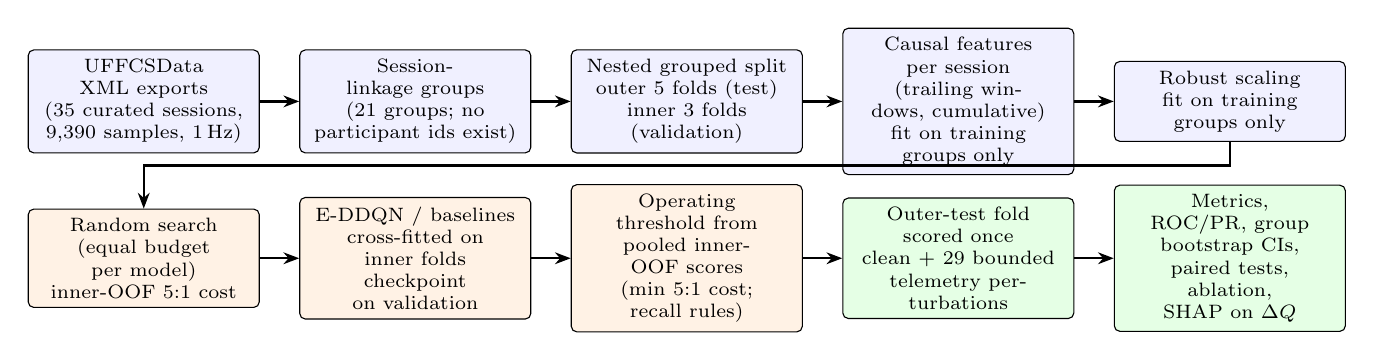
\begin{tikzpicture}[
  node distance=4mm and 5mm,
  box/.style={draw, rounded corners=2pt, align=center, font=\scriptsize, minimum height=9mm, text width=27mm, fill=#1},
  box/.default=white,
  arr/.style={-{Stealth[length=2mm]}, thick}]
\node[box=blue!6] (raw) {UFFCSData XML exports\\(\nSessionsEval{} curated sessions,\\ \nSamplesEval{} samples, 1\,Hz)};
\node[box=blue!6, right=of raw] (grp) {Session-linkage groups\\(\nGroupsEval{} groups; no\\participant ids exist)};
\node[box=blue!6, right=of grp] (split) {Nested grouped split\\outer \nOuter{} folds (test)\\inner \nInner{} folds (validation)};
\node[box=blue!6, right=of split] (feat) {Causal features per session\\(trailing windows, cumulative)\\fit on training groups only};
\node[box=blue!6, right=of feat] (scale) {Robust scaling\\fit on training groups only};
\node[box=orange!10, below=7mm of raw] (hpo) {Random search\\(equal budget per model)\\inner-OOF 5:1 cost};
\node[box=orange!10, right=of hpo] (train) {E-DDQN / baselines\\cross-fitted on inner folds\\checkpoint on validation};
\node[box=orange!10, right=of train] (thr) {Operating threshold from\\pooled inner-OOF scores\\(min 5:1 cost; recall rules)};
\node[box=green!10, right=of thr] (test) {Outer-test fold scored once\\clean + 29 bounded\\telemetry perturbations};
\node[box=green!10, right=of test] (stats) {Metrics, ROC/PR, group\\bootstrap CIs, paired tests,\\ablation, SHAP on $\Delta Q$};
\draw[arr] (raw) -- (grp);
\draw[arr] (grp) -- (split);
\draw[arr] (split) -- (feat);
\draw[arr] (feat) -- (scale);
\draw[arr] (scale.south) |- ++(0,-3mm) -| (hpo.north);
\draw[arr] (hpo) -- (train);
\draw[arr] (train) -- (thr);
\draw[arr] (thr) -- (test);
\draw[arr] (test) -- (stats);
\end{tikzpicture}
\caption{Leakage-free evaluation pipeline. Blue: data construction (no step looks across a partition boundary); orange: model development using inner (validation) folds only; green: single evaluation of each outer-test fold with the frozen protocol.}
\label{fig:pipeline}
\end{figure*}

\subsection{Data, Provenance and Target}
\label{sec:data}
The experiments use UFFCSData~\cite{porcino2019uffcsdata,porcino2022identifying,porcino2021methodology}, a public dataset in which volunteers played a race game and a flight game in a head-mounted display while the game logged, about once per second, the player's speed and acceleration, the camera orientation (quaternion components), the frame rate, the region of interest, session-configuration flags and the participant's self-reported discomfort level on a 0--3 scale; a Cybersickness Profile Questionnaire (CSPQ: gender, age band, VR experience, glasses, vision problems, eye dominance, flicker sensitivity) is stored with every session. We rebuilt every input from the original XML exports rather than from derived files. The dataset authors' curated release (\nSessionsEval{} seated sessions recorded in December~2019; \nSamplesEval{} samples) is identical, sample by sample, to \nSessionsEval{} of the raw exports and is our evaluation set. The \nSessionsDev{} standing-posture sessions recorded in October~2019 are used \emph{only} to debug code and calibrate training budgets; two further raw sessions that the dataset authors excluded are not used.

The binary target is $y_t=1$ (\emph{cybersickness event}) if the reported discomfort level at second $t$ is at least~1, and $y_t=0$ otherwise. The prevalence is \prevEval{} (Flight \prevFlight{}, Race \prevRace{}). Grades 2--3 occur in \PHGradeRaceSevere{} of \PHGradeRaceSamples{} Race samples but in only \PHGradeFlightSevere{} of \PHGradeFlightSamples{} Flight samples. Within a session the label changes rarely (on average about once), and \nEventFreeSessions{} of the \nSessionsEval{} sessions never report discomfort. We stress that $y$ marks self-reported discomfort, \emph{not} the presence of an attack: no session in the dataset was attacked.

\subsection{Unit of Independence and Splits}
\label{sec:groups}
The release contains no participant identifier, and sessions are not independent: some participants restarted after an aborted session (e.g., a 104-s session followed 108\,s later by a full session with an identical nine-field CSPQ profile). We therefore form conservative \emph{session-linkage groups}: sessions are linked if their CSPQ profiles are identical, or if a session follows an aborted one ($<200$ samples) within 180\,s with at most two differing questionnaire fields; connected components are groups. This yields \nGroupsEval{} groups. The rule may merge different people who share a profile---which only makes evaluation more conservative---but it cannot reveal one person who answered the questionnaire differently in non-consecutive sessions; we report this residual risk as a limitation.

All splits are made at the group level. A nested design is used: \nOuter{} outer folds (stratified by game and label) provide test data, and within each outer development set \nInner{} inner grouped folds provide validation data for hyper-parameter search, checkpoint selection and threshold selection. Every sample of the evaluation set is therefore predicted exactly once, by models that never saw its session, its linkage group or its exact questionnaire profile. Executable checks confirm zero session, group and profile overlap and zero duplicated feature rows between any development set and its test fold.

\subsection{Causal Feature Engineering and Preprocessing}
\label{sec:features}
Features of second $t$ use only seconds $0,\dots,t$ of the same session (verified by recomputing features on sessions truncated at random $t$). They comprise the game indicator, elapsed time, instantaneous speed, acceleration and $|$acceleration$|$, the camera quaternion components, the per-second orientation change $\lVert q_t-q_{t-1}\rVert$, the frame rate (the logger writes 0 on the very first sample of some sessions; this artifact is imputed with the training median), the region of interest, trailing-window (5\,s and 15\,s) means, standard deviations, deltas, maxima, minima, acceleration-spike rates and frame-drop fractions, and cumulative exposure descriptors (cumulative orientation change, spike and frame-drop counts, running mean speed); 39 telemetry features in total, plus 14 CSPQ indicators. The spike threshold (90th percentile of $|$acceleration$|$) and the imputation value are learned on training rows only; the frame-drop threshold (80\,fps, i.e. $>11\%$ below the 90-Hz target) is fixed. Features are scaled with a median/IQR scaler fitted on training rows. Constant or redundant columns were removed: the field of view, the static-frame and auto-camera flags are constant within each game (pure game indicators), four configuration flags and posture are constant overall, and the absolute player position was excluded because it encodes elapsed course distance and is absent in the October wave. Which of four feature sets a model uses---\emph{telemetry}, \emph{telemetry+profile}, a small a-priori \emph{exposure} set (game, elapsed time, cumulative orientation change, cumulative spikes, running and 15-s mean speed, 15-s mean rotation rate and $|$acceleration$|$), or \emph{exposure+profile}---is a hyper-parameter chosen on validation folds. Two further sets, \emph{time} (elapsed time only) and \emph{time+game}, are used only by the post-hoc baselines of Section~\ref{sec:baselines}. No oversampling or synthetic data are used anywhere; class imbalance is handled only inside training.

\subsection{Decision Formulation: MDP or Contextual Bandit?}
\label{sec:formulation}
As in DQN-based detection~\cite{lin2020imbalanced,yang2024drlimbalanced}, detection is cast as a sequential decision process over each recorded session (an \emph{episode}). The state $s_t\in\mathbb{R}^d$ is the causal feature vector at second $t$; the action $a_t\in\{0,1\}$ is \emph{stay silent} or \emph{raise an alarm}; the reward is $r_t=R(a_t,y_t)$ with
\begin{equation}
\begin{aligned}
R(1,1)&=+0.5, & R(0,0)&=+0.1,\\
R(0,1)&=-0.5, & R(1,0)&=-0.1;
\end{aligned}
\label{eq:reward}
\end{equation}
the next state $s_{t+1}$ is the next second \emph{of the same session}, and the last sample of a session is terminal. No transition ever links two sessions.

Because the telemetry was logged while participants played, without any alarm in the loop, the action cannot influence later observations: $P(s_{t+1}\mid s_t,a_t)=P(s_{t+1}\mid s_t)$. For any discount $\gamma<1$ the optimal action-value function then decomposes as
\begin{equation}
Q^*(s,a)=\mathbb{E}[R(a,y)\mid s]+\gamma\,\mathbb{E}[V^*(s_{t+1})\mid s_t=s],
\label{eq:decomp}
\end{equation}
whose second term does not depend on $a$. Hence (i) the optimal policy is myopic for every $\gamma$, i.e. the logged-data problem is a \emph{contextual bandit}~\cite{lattimore2020bandit} rather than a control problem in which actions steer future states; and (ii) with $p(s)=P(y=1\mid s)$,
\begin{equation}
Q^*(s,1)-Q^*(s,0)=p(s)\,\Delta_{\mathrm{FN}}-(1-p(s))\,\Delta_{\mathrm{FP}},
\label{eq:margin}
\end{equation}
with regrets $\Delta_{\mathrm{FN}}=R(1,1)-R(0,1)=1.0$ and $\Delta_{\mathrm{FP}}=R(0,0)-R(1,0)=0.2$. The greedy policy alarms iff $p(s)\ge \Delta_{\mathrm{FP}}/(\Delta_{\mathrm{FN}}+\Delta_{\mathrm{FP}})=1/6$, which is exactly the Bayes-optimal decision of a cost-sensitive classifier with misclassification costs $C_{\mathrm{FN}}:C_{\mathrm{FP}}=5:1$~\cite{elkan2001cost}. The asymmetric reward is therefore not a different objective from cost-sensitive learning: it encodes the same 5:1 operating point. Bootstrapping with $\gamma>0$ adds an action-independent term whose estimation noise enters both Q-values; it cannot improve the optimal policy and helps or hurts only through estimation effects. We therefore treat $\gamma\in\{0,0.5,0.9,0.99\}$ as a hyper-parameter selected on validation data and also evaluate the $\gamma=0$ special case as a separately tuned model (E-CB). A genuine MDP would require the alarm to change future rendering or symptoms (e.g., a mitigation in the loop); no such intervention exists in the data, so we make no claim that E-DDQN learns adaptive sequential control. Equation~\eqref{eq:margin} also gives every Q-learner a calibrated-probability scale, $\hat p(s)=(\Delta Q+\Delta_{\mathrm{FP}})/(\Delta_{\mathrm{FN}}+\Delta_{\mathrm{FP}})$, used to place all models on a common score scale.

\subsection{E-DDQN}
\label{sec:eddqn}
\emph{Network.} A multilayer trunk (width and depth tuned) with batch or layer normalization~\cite{ioffe2015bn}, ReLU and dropout~\cite{srivastava2014dropout} feeds a dueling head~\cite{wang2016dueling}, $Q(s,a)=V(s)+A(s,a)-\frac{1}{2}\sum_{a'}A(s,a')$, with raw (unsquashed) Q-values.
\emph{Target.} The Double-DQN target~\cite{vanhasselt2016double} with terminal flags,
\begin{equation}
y_t=r_t+\gamma(1-d_t)\,Q_{\theta^-}\big(s_{t+1},\arg\max_{a'}Q_\theta(s_{t+1},a')\big),
\end{equation}
where the online arg-max is computed in evaluation mode, and the Huber loss~\cite{girshick2015fast} is minimized with Adam~\cite{kingma2015adam}, weight decay, gradient clipping at 1.0 and a cosine learning-rate schedule~\cite{loshchilov2017sgdr}.
\emph{Target network.} Polyak averaging $\theta^-\leftarrow(1-\tau)\theta^-+\tau\theta$~\cite{lillicrap2016continuous} after every update; the batch-normalization running statistics are copied as well.
\emph{Replay.} A circular buffer~\cite{lin1992selfimproving} from which minibatches are drawn with a fixed class composition $\rho$ (Normal) and $1-\rho$ (event).
\emph{Exploration and warm-up.} $\varepsilon$-greedy exploration decaying per epoch from 1.0 to 0.01; optional warm-up with uniformly random actions.
\emph{Full-information replay.} Because labels are available offline, the reward of \emph{both} actions is known; E-DDQN may store the counterfactual action together with \emph{its own} reward, a valid transition that turns Q-learning into cost-sensitive regression of $\mathbb{E}[R\mid s,a]$. Whether to use it is tuned.
\emph{Checkpointing.} Every second epoch the agent is scored on the inner validation groups; the epoch with the lowest achievable 5:1 cost (ties: higher PR-AUC) is kept.
Algorithm~\ref{alg:eddqn} summarizes training.
\emph{Implementation pitfalls.} Three errors are easy to make when a classifier is trained as a Q-learner, and all three were present in an earlier implementation of this study: (i) building transitions across session boundaries, so that the next state of a session's last second is the first second of another session; (ii) storing the true label as the action while computing the reward of a different, exploratory action (a form of teacher forcing that trains the correct action toward the penalty of the wrong one); and (iii) averaging only the parameters into the target network, so that its batch-normalization statistics never leave their initial values. Executable unit tests guard against each of them and also verify the 5:1 regret ratio and bounded Q-values.

\begin{algorithm}[t]
\caption{E-DDQN training for one inner split}
\label{alg:eddqn}
\begin{algorithmic}[1]
\small
\State Initialize $\theta$, $\theta^-\!\leftarrow\theta$, buffer $\mathcal{D}$; optional warm-up with random actions on within-session transitions
\For{epoch $=1,\dots,E$}
  \State Concatenate training sessions in random order, each in temporal order; mark the last second of each session terminal
  \For{each chunk of 256 consecutive transitions}
    \State $a_t\gets$ $\varepsilon$-greedy on $Q_\theta(s_t,\cdot)$;\ $r_t\gets R(a_t,y_t)$
    \State store $(s_t,a_t,r_t,s_{t+1},d_t,y_t)$; if full-information replay, also store $(s_t,1-a_t,R(1-a_t,y_t),s_{t+1},d_t,y_t)$
    \State every 2 chunks: $k$ updates on class-balanced minibatches (Double-DQN target, Huber loss); Polyak update of $\theta^-$ and copy of BN statistics
  \EndFor
  \State 5 consolidation updates;\ decay $\varepsilon$;\ cosine LR step
  \State every 2 epochs: score inner-validation groups; keep $\theta$ if the achievable 5:1 cost improves
\EndFor
\State \Return checkpoint; score $\hat p(s)=(\Delta Q+\Delta_{\mathrm{FP}})/(\Delta_{\mathrm{FN}}+\Delta_{\mathrm{FP}})$
\end{algorithmic}
\end{algorithm}

\subsection{Matched Baselines}
\label{sec:baselines}
All models receive the same splits, the same four candidate feature sets, the same binary target, the same random-search budget (16 configurations; 12 for logistic regression), the same checkpoint rule (neural models), the same cross-fitted training recipe and the same threshold rules. \textbf{Standard DQN}~\cite{mnih2015human}: symmetric $\pm1$ reward, single max-operator target, periodic hard target copies (every 10, 100 or 500 updates), uniform replay, plain (non-dueling) head, same episodes and transitions; $\gamma$ is tuned as for E-DDQN. \textbf{E-CB}: E-DDQN with $\gamma=0$ (contextual bandit; the target network and double estimator are then inactive by construction). \textbf{CS-MLP}: a cost-sensitive multilayer perceptron with the same trunk family and a positive-class-weighted cross-entropy ($w=5$, i.e. the same 5:1 cost), uniform or class-balanced minibatches, checkpointed like the agents. \textbf{Logistic regression}, \textbf{histogram gradient boosting} and \textbf{random forest}~\cite{pedregosa2011sklearn} with class weight 5. For a weighted model the output $p_w$ is mapped back to $\hat p=p_w/(5-4p_w)$, so that every model's score estimates $P(y=1\mid s)$ and the Bayes cut-off is $1/6$ for all of them. Two trivial references are reported: \emph{always alarm} and \emph{never alarm}.
\emph{Post-hoc exposure-time baselines.} Because the labels are close to step functions within a session and the primary analysis selected exposure features for most models, two minimal baselines were specified after the primary analysis and run under exactly the same splits, selection, checkpoint and threshold rules and seeds: \textbf{Time-LR}, a class-weighted logistic regression on elapsed time only (all six values of $C$), and \textbf{Time+game HGB}, gradient boosting on elapsed time and the game indicator (same search space and budget as HGB). Both are reported separately from the primary comparison.

\subsection{Threat Model and Telemetry-Perturbation Stress Tests}
\label{sec:threat}
The motivating threat is an adversary who controls the rendering or locomotion pipeline (e.g., a malicious modification or compromised runtime) degrades frame pacing~\cite{odeleye2021framerate}, distorts camera or locomotion motion, or manipulates the field of view to induce or exploit cybersickness~\cite{tseng2022dark,kundu2025securing}. The dataset contains \emph{no attacked sessions} and no measurement of what any manipulation would do to a participant. We therefore evaluate only what the data support: \emph{synthetic, bounded perturbations of the logged telemetry channels} of the outer-test sessions, after which the causal features are recomputed with the frozen, training-fitted featurizer---exactly as a deployed monitor would see manipulated telemetry. Labels are never changed; an indicator $z$ marks perturbed seconds. Scenarios (frozen before evaluation): \emph{frame-rate capping} to 72/60/45\,fps (Type~I); \emph{camera-orientation jitter} $\pm0.02/0.05/0.10$ per quaternion component (Type~II); \emph{speed up-scaling} by 10/25/50\,\% with acceleration recomputed (Type~II); \emph{acceleration-spike injection} of 10/20/40 units every 20\,s (Type~II); each over the whole session or a random 60-s window, all clipped to the ranges observed in the data. \emph{Field-of-view manipulation (Type~III) is not evaluated} because the field of view never varies in the data (it is constant within each game), so any perturbation would be pure extrapolation. Two adversarial goals are analyzed with a per-session worst case over the whole-session candidates plus three ``hiding'' manipulations (speed down-scaling, orientation smoothing, frame-rate restoration): \emph{evasion} (minimize alarms on event seconds; the adversary is given the labels) and \emph{false-alarm induction} (maximize alarms on non-event seconds). Because the adversary chooses among a fixed set of candidates rather than optimizing the input, the worst cases are lower bounds on vulnerability, weaker than the gradient-based attacks of~\cite{kundu2025securing,ahmed2025adversarialvr}. Labels are kept fixed, so these tests address evasion and false-alarm induction, not the scenario in which a manipulation induces sickness and thereby changes the label. They are feature-space stress tests of the detector, not demonstrations of physical rendering attacks.

\subsection{Evaluation Protocol and Statistics}
\label{sec:protocol}
The protocol was written and committed before any model was trained on the evaluation sessions; the post-hoc analyses described at the end of this subsection were specified and committed after the primary results were known but before they were run. For every model family and outer fold, random search draws the family's configurations; each is trained on each inner split and the configuration with the lowest 5:1 expected cost on the pooled inner out-of-fold (OOF) predictions (at the cost-minimizing threshold; ties broken by PR-AUC) is selected. The selected configuration is then trained for five seeds; for each seed the \nInner{} inner models are kept (each checkpointed on its own validation groups), the outer-test score is the mean of their scores, and the operating threshold is chosen on the pooled inner-OOF scores of the development groups only. The primary operating rule (D1) minimizes the 5:1 expected cost $c=(5\,\mathrm{FN}+\mathrm{FP})/N$ on those OOF scores; secondary rules are the untuned Bayes cut-off $\hat p\ge1/6$ (D0; for the asymmetric agents this is the greedy arg-max policy) and a validation recall constraint of 0.95. Matched operating points use validation-chosen thresholds for recall targets 0.80--0.99 and specificity targets 0.5 and 0.8. The outer-test folds are never used for any choice.

We report accuracy, precision, recall, specificity, F1, balanced accuracy, MCC~\cite{chicco2020mcc}, G-mean, false-positive and false-negative rates, missed events, the 5:1 expected cost, ROC-AUC and PR-AUC~\cite{saito2015pr}, exact confusion matrices, mean~$\pm$~SD over the five seeds, and 95\,\% confidence intervals from a bootstrap that resamples linkage groups (2,000 replicates). Paired comparisons use the same test samples: McNemar's test~\cite{mcnemar1947,dietterich1998tests} (exact binomial and continuity-corrected $\chi^2$; the contingency table is checked against the error counts, $b-c=\mathrm{err}_B-\mathrm{err}_A$) and a paired group bootstrap of the cost difference. Because consecutive seconds of a session are strongly dependent, the sample-level McNemar test overstates the evidence; the group bootstrap is the primary inference. Event-level metrics (sessions whose event is detected, detection delay after onset, alarm fraction before onset and in event-free sessions) complement the per-second metrics.

\emph{Post-hoc analyses.} (i) Holm's step-down adjustment~\cite{holm1979simple} of the six group-bootstrap $p$-values comparing E-DDQN with the other primary models, per operating rule. (ii) A paired group bootstrap of each model's cost against the always-alarm policy, Holm-adjusted over models. (iii) Two grouping sensitivity analyses: a bootstrap that resamples the \nSessionsEval{} sessions instead of the \nGroupsEval{} groups, and a leave-one-group-out jackknife of every cost and cost difference. (iv) Validation-chosen cost curves: for each false-negative to false-positive ratio $R\in\{1,\dots,20\}$ the threshold minimizing $R\,\mathrm{FN}+\mathrm{FP}$ on the pooled inner-OOF scores of each outer fold is applied to that fold's test data, and the test cost is divided by the cost of the better trivial policy at the same $R$. Bootstrap $p$-values are two-sided, $2\min\{\Pr(\Delta^*\le0),\Pr(\Delta^*\ge0)\}$ over 2,000 replicates, so the smallest attainable value is about 0.001.

\subsection{Explainability}
\label{sec:shap}
SHAP values~\cite{lundberg2017shap} are computed for the decision margin $\Delta Q(s)=Q(s,1)-Q(s,0)$ of E-DDQN (one model per outer fold---the first final model of that fold---with 200 background samples drawn from its training groups and attributions for 400 of its test samples). DeepExplainer~\cite{shrikumar2017deeplift} was attempted first with its additivity check enabled; it failed that check for the selected layer-normalized networks in every fold, so the expected-gradients estimator of the SHAP library (GradientExplainer) was used instead; the method used in each fold is recorded with the released results. Attributing a single Q-value such as $Q(s,1)$ would mix in the state value $V(s)$ shared by both actions, which does not explain the decision.

\section{Experimental Setup}
\label{sec:setup}

\subsection{Implementation}
All models are implemented in PyTorch~\cite{paszke2019pytorch} and scikit-learn~\cite{pedregosa2011sklearn} and run on CPU with one thread per process. The data parser, grouping, causal features, agents, baselines, perturbation generator, protocol runner and statistics are released with the paper; one script regenerates every number from the raw XML files.

\subsection{Search Spaces and Budgets}
The search spaces (Supplementary Sec.~S2.1) are shared wherever a hyper-parameter is common to several families. Neural models: feature set (four options), trunk (64--64, 128--128, 256--256 or 256--512--256), dropout (0--0.3), normalization (batch or layer), learning rate ($3\times10^{-4}$--$3\times10^{-3}$), weight decay (0--$10^{-3}$) and batch size (256 or 512). Agents additionally: $\varepsilon$ decay per epoch (0.90--0.97), warm-up (0 or 4,000 random-action transitions) and updates per learning step (1, 2 or 4); E-DDQN: $\gamma\in\{0,0.5,0.9,0.99\}$, $\tau\in\{0.005,0.01,0.05\}$, replay composition $\rho\in\{0.4,0.5,0.6\}$ and full-information replay (on/off); E-CB: $\rho$ and full-information replay; DQN: $\gamma$ and the hard-update period (10, 100 or 500 updates); CS-MLP: uniform or class-balanced minibatches. All agents are trained for 40 epochs (one epoch is one pass over every training session in temporal order), with chunks of 256 transitions, a learning step every two chunks, five consolidation updates per epoch, a 50,000-transition buffer and gradient clipping at 1.0; the CS-MLP is trained for 40 epochs. Validation-based checkpoints are taken every two epochs. These budgets were calibrated on the October-2019 development-only sessions, where validation cost plateaued after 20--30 epochs. Each family receives \HPOBudget{} random configurations (12 for logistic regression), drawn once with a fixed seed and evaluated on every inner split of every outer fold. The same number of draws covers very different fractions of the search spaces: E-DDQN's space contains \PHSpaceEDDQN{} distinct configurations, the DQN's \PHSpaceDQN, E-CB's \PHSpaceECB{} and the CS-MLP's \PHSpaceCSMLP, against \PHSpaceHGB{} for gradient boosting, \PHSpaceRF{} for the random forest and \PHSpaceLR{} for logistic regression. The budget is therefore matched in the number of configurations, not in coverage; that a large RL search space is hard to explore with a small budget is itself a practical property of these detectors. Gradient boosting and random forests search learning rate, number of iterations, leaf counts, minimum leaf sizes, $\ell_2$ regularization, depth and feature sub-sampling; logistic regression searches the inverse regularization strength $C\in[10^{-4},10]$. The configuration selected for each outer fold is listed in Supplementary Sec.~S2.2.

\subsection{Seeds, Seed Means and the Seed Ensemble}
\label{sec:seeds}
Final models are trained with five seeds per outer fold; for every seed the outer-test score is the average of the \nInner{} cross-fitted inner models. We report mean~$\pm$~SD over seeds. Paired tests, bootstrap confidence intervals, the comparison with always alarming, event-level metrics, matched operating points, perturbation results and cost curves need a single prediction per sample; for these we use the \emph{seed ensemble}, i.e.\ the mean score over the five seeds, thresholded at the value chosen on the mean inner-OOF score. This choice was fixed in the evaluation code before the evaluation was run. Table~\ref{tab:main} reports both. They can differ, because thresholding an averaged score is not the same as averaging the metrics of separately thresholded seeds: for E-DDQN the ensemble has a higher 5:1 cost than the average seed (\PHEnsEDDQNCost{} vs.\ \EDDQNCostCostMean), whereas for the standard DQN it is lower (\PHEnsDQNCost{} vs.\ \DQNCostCostMean). Cost differences in the paired tests are therefore differences between seed ensembles and can be larger than the differences of seed means (E-DDQN vs.\ DQN: \PHEnsDiffDQN{} vs.\ \PHMeanDiffDQN). No seed was selected or discarded.

\subsection{Split-Protocol Comparison}
To quantify how the split protocol affects measured performance, we evaluated the same 21 raw columns of the curated release under three protocols with an untuned gradient-boosting classifier: (i) oversampling every discomfort grade to the size of grade~0 (5,243 samples) \emph{before} a random 70/15/15 row-level split, the protocol of the earlier, unpublished version of this study (it reproduces that version's partition sizes, 14,680 / 3,146 / 3,146, exactly); (ii) a row-level split without oversampling; and (iii) the grouped split of Section~\ref{sec:groups}. The earlier E-DDQN implementation was also run, unmodified, on partitions (i) and (iii). Because that version's 41-feature input files were not available, this is a reconstruction of its protocol rather than an exact reproduction.

\section{Results}
\label{sec:results}

\subsection{Effect of the Split Protocol (RQ1)}
\label{sec:leak}
Table~\ref{tab:leak} evaluates the same 21 raw columns under three protocols. When every discomfort grade is oversampled to 5,243 samples before a 70/15/15 row split, an untuned gradient-boosting classifier reaches \LeakOldAcc\,\% accuracy, \LeakOldRecall\,\% recall, MCC \LeakOldMCC{} and ROC-AUC \LeakOldRocAuc; \LeakDupPos{} of the \LeakTestPos{} positive test rows (\LeakDupPct\,\%) have an exact duplicate in the training split, and every session contributes to both splits. Without oversampling, a row-level split still gives ROC-AUC \LeakRowRocAuc{} (accuracy \LeakRowAcc\,\%), because adjacent seconds of the same session are nearly identical and carry the same label. With a session-grouped split, the same classifier falls to ROC-AUC \LeakGrpRocAuc{} (MCC \LeakGrpMCC). The earlier E-DDQN implementation behaves the same way: \OrigOldRecall\,\% recall and MCC \OrigOldMCC{} on the oversampled row-level partition, but MCC \OrigGrpMCC{} on a grouped partition. Near-perfect scores on these data therefore measure the recognition of sessions seen during training, not the detection of cybersickness in new sessions, and they are obtained without any reinforcement learning. All results below use the leakage-free protocol of Section~\ref{sec:protocol}.

\begin{table*}[t]
\centering
\caption{Effect of the evaluation protocol on the same data (21 raw columns of the curated release; test-split metrics). ``Proxy'' marks the reconstruction of the earlier protocol, whose 41-feature input files were not available.}
\label{tab:leak}
\resizebox{\textwidth}{!}{\begin{tabular}{llccccc}
\toprule
Model & Evaluation protocol & Acc. & Recall & Spec. & MCC & ROC-AUC \\
\midrule
HGB & Oversample to 5,243/grade, then 70/15/15 row split (earlier protocol) & 97.6 & 99.8 & 91.0 & 0.935 & 0.995 \\
HGB & Row-level random split, no oversampling & 95.3 & 94.1 & 96.3 & 0.905 & 0.992 \\
HGB & Grouped 5-fold split (session-linkage groups) & 52.2 & 33.6 & 66.9 & 0.005 & 0.523 \\
E-DDQN (earlier code) & Earlier script, earlier protocol (proxy) & 95.2 & 99.2 & 83.1 & 0.870 & -- \\
E-DDQN (earlier code) & Earlier script, grouped split (proxy) & 41.1 & 92.1 & 7.7 & $-$0.004 & -- \\
\bottomrule
\end{tabular}
}
\end{table*}

\subsection{Leakage-Free Comparison under the 5:1 Cost (RQ3)}
\label{sec:main}
Table~\ref{tab:main} reports every model tuned, checkpointed and thresholded on validation groups only and scored once on the outer-test groups (all \nSamplesEval{} samples, \nSessionsEval{} sessions). Two facts dominate. First, the detection problem is hard once sessions and participants are not shared: among the primary models, the best ROC-AUC is \HGBCostRocAucMean{} (HGB) and \RFCostRocAucMean{} (random forest), against a prevalence of 0.44. Second, under a 5:1 cost the cost-minimizing operating point of every model lies close to ``always alarm'' (cost \AlwaysCost): validation-selected thresholds yield high recall but false-positive rates of \DOneFPRMin--\DOneFPRMax\,\%. The random forest has the lowest cost, both as a mean over seeds (\RFCostCostMean$\pm$\RFCostCostSD) and as a seed ensemble (\PHEnsRFCost).

E-DDQN ranks last of the \nModels{} primary models: recall \EDDQNCostRecallMean$\pm$\EDDQNCostRecallSD\,\%, specificity \EDDQNCostSpecMean$\pm$\EDDQNCostSpecSD\,\%, cost \EDDQNCostCostMean$\pm$\EDDQNCostCostSD{} (higher than always alarming), ROC-AUC \EDDQNCostRocAucMean$\pm$\EDDQNCostRocAucSD{} and MCC \EDDQNCostMCCMean; its seed ensemble is worse still (cost \PHEnsEDDQNCost, recall \PHEnsEDDQNRecall\,\%). The standard DQN reaches cost \DQNCostCostMean{} and ROC-AUC \DQNCostRocAucMean, and the contextual-bandit variant E-CB cost \ECBCostCostMean{} and ROC-AUC \ECBCostRocAucMean. E-DDQN therefore does not improve on the standard DQN in this controlled comparison.

\begin{table*}[t]
\centering
\caption{Leakage-free comparison (rule D1: threshold minimizing the 5:1 cost on pooled inner-validation predictions; \nSamplesEval{} outer-test samples; recall, specificity and balanced accuracy in \%). Left: mean~$\pm$~SD over five seeds. Right: the seed ensemble (mean score over the five seeds, thresholded on the mean inner-OOF score; Section~\ref{sec:seeds}), whose predictions are used for the paired tests, confidence intervals, comparison with always alarming and cost curves; FN and FP are exact counts. Bold: lowest cost among the primary models. HGB, logistic regression and the post-hoc baselines are deterministic given the data, hence SD = 0 and identical left and right values. Precision, F1, accuracy and G-mean: Supplementary Sec.~S3.1.}
\label{tab:main}
\resizebox{\textwidth}{!}{\begin{tabular}{lccccccc|ccccc}
\toprule
 & \multicolumn{7}{c|}{Mean $\pm$ SD over five seeds} & \multicolumn{5}{c}{Seed ensemble (paired tests)} \\
Model & Recall & Spec. & Bal.\ acc. & MCC & Cost$_{5:1}$ & ROC-AUC & PR-AUC & Recall & Spec. & Cost$_{5:1}$ & FN & FP \\
\midrule
\textbf{E-DDQN} & 93.4$\pm$2.5 & 7.4$\pm$2.7 & 50.4$\pm$1.2 & 0.016$\pm$0.054 & 0.663$\pm$0.048 & 0.538$\pm$0.016 & 0.483$\pm$0.019 & 90.4 & 8.1 & 0.726 & 400 & 4,820 \\
E-CB & 97.1$\pm$2.9 & 8.4$\pm$2.8 & 52.8$\pm$1.2 & 0.122$\pm$0.052 & 0.575$\pm$0.055 & 0.653$\pm$0.011 & 0.562$\pm$0.006 & 96.6 & 14.6 & 0.552 & 140 & 4,480 \\
DQN & 95.2$\pm$2.7 & 14.5$\pm$4.9 & 54.8$\pm$1.6 & 0.158$\pm$0.038 & 0.584$\pm$0.040 & 0.661$\pm$0.013 & 0.595$\pm$0.022 & 96.9 & 16.3 & 0.536 & 129 & 4,391 \\
CS-MLP & 99.4$\pm$0.7 & 2.8$\pm$1.9 & 51.1$\pm$0.8 & 0.072$\pm$0.049 & 0.557$\pm$0.012 & 0.644$\pm$0.018 & 0.521$\pm$0.022 & 99.4 & 6.1 & 0.537 & 23 & 4,925 \\
LogReg & 99.1$\pm$0.0 & 8.1$\pm$0.0 & 53.6$\pm$0.0 & 0.167$\pm$0.000 & 0.532$\pm$0.000 & 0.626$\pm$0.000 & 0.576$\pm$0.000 & 99.1 & 8.1 & 0.532 & 36 & 4,817 \\
HGB & 97.0$\pm$0.0 & 14.6$\pm$0.0 & 55.8$\pm$0.0 & 0.197$\pm$0.000 & 0.543$\pm$0.000 & 0.692$\pm$0.000 & 0.593$\pm$0.000 & 97.0 & 14.6 & 0.543 & 124 & 4,479 \\
RF & 98.5$\pm$0.3 & 18.2$\pm$0.7 & 58.3$\pm$0.3 & 0.266$\pm$0.004 & \textbf{0.491$\pm$0.003} & 0.688$\pm$0.002 & 0.548$\pm$0.001 & 98.7 & 18.3 & \textbf{0.485} & 54 & 4,281 \\
\midrule
\multicolumn{13}{l}{\emph{Post-hoc exposure-time baselines (added after the primary analysis)}} \\
Time-LR (elapsed time) & 96.7$\pm$0.0 & 15.0$\pm$0.0 & 55.8$\pm$0.0 & 0.194$\pm$0.000 & 0.548$\pm$0.000 & 0.704$\pm$0.000 & 0.605$\pm$0.000 & 96.7 & 15.0 & 0.548 & 138 & 4,457 \\
Time+game HGB & 97.4$\pm$0.0 & 17.6$\pm$0.0 & 57.5$\pm$0.0 & 0.239$\pm$0.000 & 0.517$\pm$0.000 & 0.676$\pm$0.000 & 0.550$\pm$0.000 & 97.4 & 17.6 & 0.517 & 107 & 4,319 \\
\midrule
Always alarm & 100.0 & 0.0 & 50.0 & 0.000 & 0.558 & -- & -- & 100.0 & 0.0 & 0.558 & 0 & 5,243 \\
Never alarm & 0.0 & 100.0 & 50.0 & 0.000 & 2.208 & -- & -- & 0.0 & 100.0 & 2.208 & 4,147 & 0 \\
\bottomrule
\end{tabular}
}
\end{table*}

\subsection{Exposure-Time Baselines}
\label{sec:time}
The post-hoc baselines (Table~\ref{tab:main}, Fig.~\ref{fig:roc}) show what the primary models have learned. Time-LR, a logistic regression on elapsed time alone, reaches ROC-AUC \PHTimeLRRocAucMean{} and PR-AUC \PHTimeLRPrAucMean, the highest values of all models. Its ROC-AUC does not differ significantly from that of the random forest (difference \PHTimeLRvsRFAuc, 95\,\% CI \PHTimeLRvsRFAucLow{} to \PHTimeLRvsRFAucHigh; group bootstrap); the interval is wide, so equivalence is not established either. At the 5:1 operating point, however, the random forest has a lower cost than Time-LR (seed ensembles \PHEnsRFCost{} vs.\ \PHEnsTimeLRCost; difference \PHTimeLRvsRFCost, CI \PHTimeLRvsRFCostLow{} to \PHTimeLRvsRFCostHigh, $p=$\,\PHTimeLRvsRFCostP), so the additional inputs help the forest at the operating point (fewer missed events and fewer false alarms in the seed ensemble; Table~\ref{tab:main}). Adding the game indicator (Time+game HGB) gives cost \PHTimeHGBCostMean{} and ROC-AUC \PHTimeHGBRocAucMean, again not significantly different from the random forest (cost difference \PHTimeHGBvsRFCost, $p=$\,\PHTimeHGBvsRFCostP; ROC-AUC difference \PHTimeHGBvsRFAuc, $p=$\,\PHTimeHGBvsRFAucP). Both minimal baselines rank seconds better than E-DDQN (seed-ensemble ROC-AUC difference for Time-LR \PHTimeLRvsEDDQNAuc, CI \PHTimeLRvsEDDQNAucLow{} to \PHTimeLRvsEDDQNAucHigh). On these data, therefore, no model was shown to discriminate better than a population onset curve, in which cybersickness becomes more likely the longer a session lasts; the wide intervals leave open modest gains that a sample of \nGroupsEval{} groups cannot detect.

\begin{figure}[t]
\centering
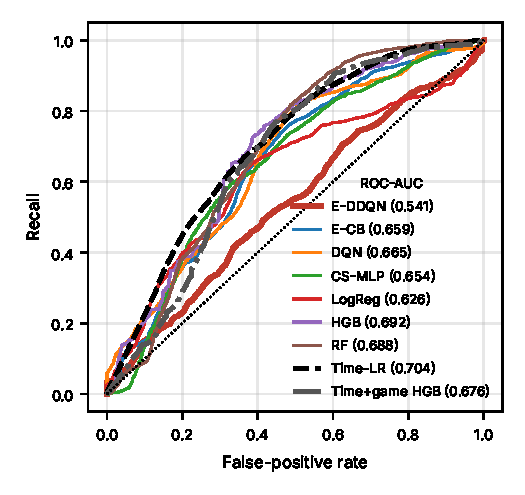
\includegraphics[width=\columnwidth]{figs/posthoc_roc.pdf}
\caption{ROC curves of the seed-ensemble scores, pooled over the five outer-test folds, for the seven primary models and the two post-hoc exposure-time baselines (dashed and dash-dotted). The legend gives the ROC-AUC of the seed-ensemble score, which can differ slightly from the seed means in Table~\ref{tab:main}.}
\label{fig:roc}
\end{figure}

\subsection{Operating Points, Cost Ratios and the Asymmetric Reward}
\label{sec:op}
Table~\ref{tab:ops} contrasts three operating rules. With the untuned Bayes cut-off $\hat p\ge 1/6$ (rule D0)---for the asymmetric agents this is the greedy policy $\arg\max_a Q(s,a)$---E-DDQN obtains recall \EDDQNBayesRecallMean\,\% at specificity \EDDQNBayesSpecMean\,\% (cost \EDDQNBayesCostMean), whereas the random forest obtains recall \RFBayesRecallMean\,\% at specificity \RFBayesSpecMean\,\% (cost \RFBayesCostMean). When every model is held to a validation recall of at least 0.95, the random forest again has the lowest cost (\RFRecCostMean; E-DDQN \EDDQNRecCostMean). At validation-matched recall targets (Table~\ref{tab:matched}), the thresholds transfer worst for E-DDQN: at both recall targets it attains lower test recall than every supervised model, and at the 0.95 target it also has a higher false-positive rate than all of them. Reading the ROC curves at fixed recall (descriptive only), the false-positive rate at 95\,\% recall is \EDDQNRocFPRatNineFive\,\% for E-DDQN and \RFRocFPRatNineFive\,\% for the random forest. Because the reward encodes the same 5:1 operating point as a cost-weighted classifier (Eq.~\eqref{eq:margin}), the asymmetric reward provides no advantage that cost-weighted training plus a validation-selected threshold does not already provide.

The cost curves of Fig.~\ref{fig:costcurves} show how much the choice of the 5:1 ratio matters. At ratios of 1.5--2, where the cost-optimal policy is not close to a trivial one, the relative costs of all models except E-DDQN lie between \PHCcLowRMin{} and \PHCcLowRMax{} (random forest: \PHCcRFTwo{} at $R=2$). As $R$ grows, every curve approaches 1, because the Bayes cut-off $1/(1+R)$ falls far below the prevalence and alarming almost always becomes optimal; at $R=5$ the random forest's relative cost is \PHCcRFFive. The random forest stays below the trivial policies at all \PHCcNratios{} ratios, E-DDQN at \PHCcEDDQNBelow{} of them. The negative safety result is therefore not an artifact of the particular ratio: the models discriminate weakly at every ratio, and the 5:1 ratio places the operating point where that weakness is most visible.

\begin{figure}[t]
\centering
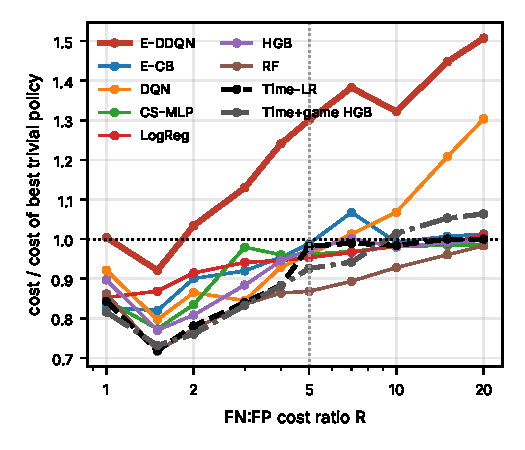
\includegraphics[width=\columnwidth]{figs/posthoc_cost_curves.pdf}
\caption{Validation-chosen cost curves (post hoc): for each false-negative to false-positive cost ratio $R$, the threshold minimizing $R\,\mathrm{FN}+\mathrm{FP}$ on the inner-validation predictions is applied to the outer-test fold; the pooled test cost of the seed ensemble is divided by the cost of the better trivial policy (always or never alarm). Values below 1 improve on the trivial policy; the dotted vertical line marks the 5:1 ratio.}
\label{fig:costcurves}
\end{figure}

\begin{table}[t]
\centering
\caption{Expected 5:1 cost (mean over seeds) under three operating rules chosen without test data.}
\label{tab:ops}
\footnotesize
\begin{tabular}{lccc}
\toprule
Model & D1: min cost & D0: $\hat p\ge 1/6$ & val.\ recall $\ge$ 0.95 \\
\midrule
E-DDQN & \EDDQNCostCostMean & \EDDQNBayesCostMean & \EDDQNRecCostMean \\
E-CB & \ECBCostCostMean & \ECBBayesCostMean & \ECBRecCostMean \\
DQN & \DQNCostCostMean & \DQNBayesCostMean & \DQNRecCostMean \\
CS-MLP & \CSMLPCostCostMean & \CSMLPBayesCostMean & \CSMLPRecCostMean \\
LogReg & \LRCostCostMean & \LRBayesCostMean & \LRRecCostMean \\
HGB & \HGBCostCostMean & \HGBBayesCostMean & \HGBRecCostMean \\
RF & \RFCostCostMean & \RFBayesCostMean & \RFRecCostMean \\
\midrule
Always alarm & \AlwaysCost & \AlwaysCost & \AlwaysCost \\
\bottomrule
\end{tabular}
\end{table}

\begin{table*}[t]
\centering
\caption{Matched operating points: thresholds chosen on validation predictions to reach the stated recall or specificity; test recall (\%), false-positive rate (\%) and false-positive count of the seed ensemble.}
\label{tab:matched}
\footnotesize
\begin{tabular}{lccccccccc}
\toprule
 & \multicolumn{3}{c}{val. recall $\ge$ 0.90} & \multicolumn{3}{c}{val. recall $\ge$ 0.95} & \multicolumn{3}{c}{val. specificity $\ge$ 0.80} \\
Model & Rec. & FPR & FP & Rec. & FPR & FP & Rec. & FPR & FP \\
\midrule
E-DDQN & 81.7 & 77.0 & 4,036 & 84.5 & 86.6 & 4,539 & 25.2 & 18.6 & 974 \\
E-CB & 88.6 & 68.0 & 3,565 & 92.4 & 78.1 & 4,093 & 31.2 & 17.4 & 910 \\
DQN & 88.0 & 64.2 & 3,366 & 91.7 & 72.7 & 3,810 & 32.2 & 14.2 & 743 \\
CS-MLP & 94.1 & 78.4 & 4,111 & 97.5 & 85.1 & 4,463 & 24.2 & 12.7 & 666 \\
LogReg & 92.8 & 73.5 & 3,856 & 97.2 & 81.7 & 4,285 & 37.7 & 22.5 & 1,181 \\
HGB & 95.4 & 72.2 & 3,785 & 97.5 & 81.7 & 4,282 & 24.3 & 11.3 & 594 \\
RF & 93.7 & 64.0 & 3,358 & 96.9 & 74.3 & 3,896 & 21.0 & 13.3 & 695 \\
\bottomrule
\end{tabular}

\end{table*}

\subsection{Statistical Comparison}
\label{sec:stats}
Table~\ref{tab:paired} compares E-DDQN with every other primary model on identical test samples (seed ensembles, rule D1). Sample-level McNemar tests give $p<0.001$ for every pair, but they treat \nSamplesEval{} strongly autocorrelated seconds as independent and overstate the evidence; they are reported for completeness, with the contingency identity $b-c=\mathrm{err}_B-\mathrm{err}_A$ checked and recomputed with an independent library. The primary inference is the group bootstrap, which resamples the \nGroupsEval{} independent units. E-DDQN's seed-ensemble cost (\PHEnsEDDQNCost) exceeds that of every other primary model by \PairDOneECBCostDiff{} to \PairDOneRFCostDiff. These ensemble differences are larger than the corresponding differences of seed means in Table~\ref{tab:main} (\PHMeanDiffDQN{} to \PHMeanDiffRF) because E-DDQN's ensemble is worse than its average seed (Section~\ref{sec:seeds}); after Holm adjustment over the six comparisons, only the difference from the random forest remains significant (\PairDOneRFCostDiff, 95\,\% CI \PairDOneRFCostLo{} to \PairDOneRFCostHi; adjusted $p=$\,\PHHolmRF), whereas the adjusted $p$-values for the other five comparisons lie between \PHHolmECB{} and \PHHolmHGB. In particular, the difference from the standard DQN (\PairDOneDQNCostDiff; seed means \PHMeanDiffDQN) is not significant (unadjusted $p=$\,\PairDOneDQNPboot).

These conclusions are robust to the choice of resampling unit and to individual groups. Resampling the \nSessionsEval{} sessions instead of the groups gives the same pattern (E-DDQN vs.\ random forest: CI \PHSesRFLow{} to \PHSesRFHigh, Holm-adjusted $p=$\,\PHSesRFHolm). In a leave-one-group-out jackknife over the \PHJkGroups{} groups, the cost difference between E-DDQN and the random forest ranges from \PHJkEDDQNvsRFMin{} to \PHJkEDDQNvsRFMax{} and never changes sign; the same holds for every other comparison with E-DDQN. Compared with always alarming, the random forest's seed-ensemble cost differs by \PHAlwRFGrp{} (CI \PHAlwRFGrpLow{} to \PHAlwRFGrpHigh; unadjusted $p=$\,\PHAlwRFGrpP), but after Holm adjustment over the nine models this is not significant ($p=$\,\PHAlwRFGrpHolm); E-DDQN's seed-ensemble cost differs from that of always alarming by \PHAlwEDDQNGrp{} (CI \PHAlwEDDQNGrpLow{} to \PHAlwEDDQNGrpHigh). No model is therefore shown to improve on the trivial policy at the 5:1 ratio.

\begin{table*}[t]
\centering
\caption{Paired comparisons with E-DDQN (A) on the same \nSamplesEval{} test samples (seed ensembles, rule D1). $b$: A correct, B wrong; $c$: A wrong, B correct. $\Delta$Cost is the difference of the seed-ensemble costs (Table~\ref{tab:main}, right block); its CI and $p_{\text{group}}$ come from 2,000 group-bootstrap replicates (unadjusted; Holm-adjusted values in the text); $p_{\text{exact}}$ is the sample-level exact McNemar test, which ignores within-session dependence.}
\label{tab:paired}
\footnotesize
\begin{tabular}{lcccccccc}
\toprule
B (vs. A = E-DDQN) & $b$ & $c$ & err$_A$ & err$_B$ & $\chi^2_{cc}$ & $p_{\text{exact}}$ & $\Delta$Cost$_{5:1}$ (A$-$B) [95\% CI] & $p_{\text{group}}$ \\
\midrule
E-CB & 299 & 899 & 5,220 & 4,620 & 299.5 & $<$0.001 & +0.175 [+0.016, +0.448] & 0.014 \\
DQN & 297 & 997 & 5,220 & 4,520 & 377.6 & $<$0.001 & +0.190 [$-$0.017, +0.493] & 0.079 \\
CS-MLP & 402 & 674 & 5,220 & 4,948 & 68.3 & $<$0.001 & +0.190 [+0.005, +0.485] & 0.039 \\
LogReg & 389 & 756 & 5,220 & 4,853 & 117.0 & $<$0.001 & +0.194 [+0.011, +0.477] & 0.026 \\
HGB & 203 & 820 & 5,220 & 4,603 & 370.9 & $<$0.001 & +0.183 [+0.011, +0.460] & 0.035 \\
RF & 293 & 1,178 & 5,220 & 4,335 & 531.2 & $<$0.001 & +0.242 [+0.052, +0.528] & 0.001 \\
\bottomrule
\end{tabular}

\end{table*}

\subsection{Event-Level Behavior}
At the cost-optimal operating points (seed ensembles) every model flags almost every session: E-DDQN raises an alarm on \EDDQNEvFreeAlarm\,\% of the seconds of the \nEventFreeSessions{} sessions in which no discomfort was ever reported and on \EDDQNEvPreAlarm\,\% of the seconds before onset in the \nEventSessions{} sessions with an event (random forest: \RFEvFreeAlarm\,\% and \RFEvPreAlarm\,\%). Events are therefore ``detected'' with zero median delay by construction, not through discrimination.

\subsection{Why E-DDQN Under-Performs: Bootstrapping and Selection Optimism}
\label{sec:why}
Validation selected $\gamma=$ \EDDQNGammas{} for the five outer folds of E-DDQN, i.e.\ strong bootstrapping, and the exposure+profile feature set in \EDDQNnProfile{} of 5 folds. Section~\ref{sec:formulation} shows that bootstrapping cannot improve the optimal policy here and adds action-independent estimation noise to $\Delta Q$. Two diagnostics agree. (i) The separately tuned $\gamma=0$ variant (E-CB) ranks much better (ROC-AUC \ECBCostRocAucMean{} vs.\ \EDDQNCostRocAucMean). (ii) Table~\ref{tab:optimism} compares, per family, the inner-validation cost of the configuration at the moment it was selected with its outer-test cost. The gap is \EDDQNOptGap{} for E-DDQN but between \RFOptGap{} and \ECBOptGap{} for all other models: noisy, high-variance training curves combined with validation checkpointing and selection let E-DDQN configurations look best on validation folds by chance~\cite{varma2006bias}. Q-value estimates stay finite, so the failure is not numerical divergence, but they are poorly scaled. The largest magnitude over all E-DDQN runs is \EDDQNQAbsMax{} (DQN \DQNQAbsMax, E-CB \ECBQAbsMax), and relative to the return bound $r_{\max}/(1-\gamma)$ of each fold's selected discount the largest estimates exceed the bound by up to a factor of \PHQRatioMaxEDDQN{} for E-DDQN (in \PHQRatioFoldsEDDQN{} of 5 folds), \PHQRatioMaxDQN{} for DQN and \PHQRatioMaxECB{} for E-CB, i.e.\ extrapolation on atypical states. The mean greedy-action Q-value differs from its realized discounted validation return by \EDDQNOverest{} for E-DDQN, \DQNOverest{} for DQN and \ECBOverest{} for E-CB.

\begin{table}[t]
\centering
\caption{Selection optimism: pooled inner-validation 5:1 cost of the selected configuration (HPO seed) versus its outer-test cost (mean over folds and seeds).}
\label{tab:optimism}
\footnotesize
\begin{tabular}{lccc}
\toprule
Model & Inner-OOF cost at selection & Outer-test cost & Gap \\
\midrule
E-DDQN & 0.467 & 0.754 & +0.288 \\
E-CB & 0.488 & 0.557 & +0.070 \\
DQN & 0.478 & 0.544 & +0.065 \\
CS-MLP & 0.501 & 0.534 & +0.033 \\
LogReg & 0.518 & 0.531 & +0.014 \\
HGB & 0.518 & 0.539 & +0.021 \\
RF & 0.495 & 0.481 & $-$0.015 \\
\bottomrule
\end{tabular}

\end{table}

\subsection{Component Ablation and Reward-Ratio Sensitivity}
\label{sec:ablation}
Table~\ref{tab:ablation} removes or changes one component of E-DDQN at a time while keeping the configuration selected for each outer fold fixed (five seeds; same protocol). Every variant ranks close to chance (ROC-AUC \AblSoftCostRocAuc--\AblGammaZeroCostRocAuc). No single change moves the cost by more than about one seed standard deviation of the full model (\EDDQNCostCostMean$\pm$\EDDQNCostCostSD). The lowest cost is obtained by \emph{replacing} the asymmetric reward with the symmetric $\pm1$ reward (\AblAsymCostCost) and the highest ROC-AUC by switching off bootstrapping ($\gamma=0$; \AblGammaZeroCostRocAuc); hard target copies (\AblSoftCostCost), no dueling head (\AblDuelCostCost), uniform replay (\AblBalCostCost), no warm-up (\AblWarmCostCost) and toggling full-information replay (\AblFullCostCost) leave the cost essentially unchanged, and removing the double estimator slightly increases it (\AblDoubleCostCost). None of these components can be credited with a gain in safety or accuracy. Every variant is scored on the same implied-probability scale and thresholded with the same rules, so the reward table can act only through the learned scores; at the fixed cut-off $\hat p\ge1/6$ (rule D0) the symmetric-reward variant is not worse either (cost \AblAsymBayesCost{} vs.\ \EDDQNBayesCostMean).

\begin{table*}[t]
\centering
\caption{Leave-one-component-out ablation of E-DDQN (selected configuration per outer fold held fixed; rule D1; mean over 5 seeds, cost $\pm$ SD).}
\label{tab:ablation}
\footnotesize
\begin{tabular}{lccccc}
\toprule
Variant & Recall & Spec. & Cost$_{5:1}$ & ROC-AUC & PR-AUC \\
\midrule
Full E-DDQN (selected) & 93.4 & 7.4 & 0.663$\pm$0.048 & 0.538 & 0.483 \\
\midrule
full-information replay toggled & 93.7 & 5.4 & 0.667$\pm$0.106 & 0.563 & 0.500 \\
symmetric $\pm$1 reward instead of asymmetric & 94.8 & 8.6 & 0.625$\pm$0.038 & 0.572 & 0.517 \\
uniform instead of class-balanced replay & 94.3 & 4.3 & 0.660$\pm$0.045 & 0.554 & 0.486 \\
no double estimator (max-operator target) & 93.1 & 5.3 & 0.681$\pm$0.086 & 0.543 & 0.491 \\
no dueling head & 94.6 & 5.8 & 0.644$\pm$0.059 & 0.559 & 0.494 \\
hard target copy every 10 updates & 94.9 & 6.5 & 0.634$\pm$0.043 & 0.529 & 0.472 \\
no warm-up & 93.8 & 7.1 & 0.656$\pm$0.049 & 0.547 & 0.497 \\
$\gamma=0$ (contextual bandit) & 94.4 & 6.4 & 0.645$\pm$0.070 & 0.576 & 0.510 \\
\bottomrule
\end{tabular}

\end{table*}

Table~\ref{tab:ratio} varies the false-negative to false-positive regret of the reward from 1:1 to 10:1 (E-DDQN configuration per fold fixed; ratio 5:1 reproduces the main E-DDQN run bit for bit, which also confirms the determinism of the pipeline). The greedy policy moves along the trade-off in the direction Eq.~\eqref{eq:margin} predicts (its nominal cut-off is $1/(1+R)$; because of class-balanced replay it corresponds approximately to $1/(1+kR)$ on $P(y=1\mid s)$, with $k=$ \SSEDDQNKMin--\SSEDDQNKMax{} over the inner models of the selected E-DDQN configurations, Section~\ref{sec:formulation}): recall rises from \RatioArgOneRecall\,\% (1:1) to \RatioArgFiveRecall\,\% (5:1) and \RatioArgOneZeroRecall\,\% (10:1), while specificity falls from \RatioArgOneSpec\,\% to \RatioArgFiveSpec\,\% and \RatioArgOneZeroSpec\,\%. Once the threshold is chosen on validation data, however, all ratios end at similar costs (\RatioTunedOneCost--\RatioTunedOneZeroCost; the largest difference is smaller than any ratio's seed standard deviation, and no formal test was performed) and similar ranking: the reward ratio sets the default operating point, but it does not create discrimination that a threshold cannot reproduce. The 5:1 ratio is therefore best understood as a declared safety preference whose operating point can equally be reached by cost-weighted training or threshold selection.

\begin{table*}[t]
\centering
\caption{Reward-ratio sensitivity of E-DDQN: operating point of the greedy (arg-max) policy, whose nominal cut-off is $1/(1+R)$ ($1/(1+kR)$ on $P(y=1\mid s)$ under class-balanced replay; Section~\ref{sec:formulation}), and of the validation-tuned threshold (rule D1). Mean ($\pm$ SD) over five seeds.}
\label{tab:ratio}
\footnotesize
\input{generated/tab_ratio_policy.tex}
\end{table*}



\subsection{Robustness under Telemetry Perturbations (RQ4)}
\label{sec:attack}
Table~\ref{tab:attack-auc} reports threshold-free ranking performance under each perturbation fixed before evaluation. \AttAucFracSmall\,\% of the model--scenario combinations change the pooled ROC-AUC by less than 0.03 and none by more than \AttAucMaxAbsChange{} (the largest drops occur for acceleration-spike injection in E-CB and DQN and for speed down-scaling in gradient boosting), and several perturbations even raise it slightly. This insensitivity is not evidence of a robust safety monitor: it arises because the dominant inputs selected on validation data are exposure time, cumulative exposure and questionnaire answers rather than the manipulated channels, and the exposure-time baselines, whose inputs no perturbation touches, are perfectly insensitive by construction. At the cost-optimal operating points (Table~\ref{tab:attack}), the per-session worst-case evasion adversary lowers recall on event seconds from \EDDQNAttCleanRecall\,\% to \EDDQNAttWorstRecall\,\% for E-DDQN, from \ECBAttCleanRecall\,\% to \ECBAttWorstRecall\,\% for E-CB and from \RFAttCleanRecall\,\% to \RFAttWorstRecall\,\% for the random forest, while the false-alarm adversary drives the false-positive rate of every model to \EDDQNAttWorstFPR--100\,\% (it is already \RFAttCleanFPR--\CSMLPAttCleanFPR\,\% without manipulation). These are lower bounds from a weak, candidate-selecting adversary on feature-space perturbations; they do not show what a real rendering attack would do to a participant, and field-of-view manipulation cannot be evaluated because the field of view never varies in the data.

\begin{table*}[t]
\centering
\caption{Threshold-free robustness: pooled outer-test ROC-AUC of the seed-ensemble score on clean telemetry and under whole-session perturbations (the last column gives the most negative and most positive change over all 21 whole-session variants).}
\label{tab:attack-auc}
\footnotesize
\begin{tabular}{lcccccccc}
\toprule
Model & Clean & fps$\le$45 & jitter 0.10 & speed $\times$1.5 & spikes 40 & speed $\times$0.5 & smooth 0.25 & min / max $\Delta$ \\
\midrule
E-DDQN & 0.541 & 0.541 & 0.593 & 0.561 & 0.559 & 0.532 & 0.539 & $-$0.008 / +0.053 \\
E-CB & 0.659 & 0.659 & 0.682 & 0.648 & 0.575 & 0.648 & 0.658 & $-$0.089 / +0.052 \\
DQN & 0.665 & 0.665 & 0.677 & 0.680 & 0.605 & 0.632 & 0.676 & $-$0.064 / +0.035 \\
CS-MLP & 0.654 & 0.649 & 0.654 & 0.630 & 0.652 & 0.629 & 0.646 & $-$0.025 / +0.005 \\
LogReg & 0.626 & 0.677 & 0.639 & 0.620 & 0.629 & 0.608 & 0.639 & $-$0.017 / +0.051 \\
HGB & 0.692 & 0.694 & 0.709 & 0.650 & 0.698 & 0.647 & 0.712 & $-$0.068 / +0.019 \\
RF & 0.688 & 0.689 & 0.708 & 0.667 & 0.683 & 0.723 & 0.725 & $-$0.021 / +0.037 \\
\bottomrule
\end{tabular}

\end{table*}

\begin{table*}[t]
\centering
\caption{Recall/false-positive rate (\%) of the seed ensembles on perturbed seconds at the D1 operating point, and per-session adaptive worst cases (evasion: minimum recall; false-alarm induction: maximum FPR) over all whole-session candidates.}
\label{tab:attack}
\footnotesize
\begin{tabular}{lcccccccc}
\toprule
 & Clean & fps$\le$45 & jitter 0.10 & speed $\times$1.5 & spikes 40 & \multicolumn{2}{c}{Adaptive worst case} \\
Model & Rec./FPR & Rec./FPR & Rec./FPR & Rec./FPR & Rec./FPR & Rec. (evasion) & FPR (false alarm) \\
\midrule
E-DDQN & 90.4/91.9 & 90.4/91.9 & 94.0/92.2 & 93.5/90.7 & 95.4/94.3 & 82.9 & 94.5 \\
E-CB & 96.6/85.4 & 96.6/85.4 & 96.1/88.2 & 98.7/95.9 & 99.3/97.7 & 78.0 & 98.9 \\
DQN & 96.9/83.7 & 96.9/83.7 & 94.8/83.5 & 97.8/91.8 & 97.9/95.4 & 87.3 & 97.5 \\
CS-MLP & 99.4/93.9 & 100.0/98.3 & 99.7/96.5 & 100.0/98.2 & 99.9/99.1 & 95.6 & 100.0 \\
LogReg & 99.1/91.9 & 97.0/86.3 & 99.2/92.7 & 99.7/94.9 & 99.9/96.7 & 95.4 & 96.7 \\
HGB & 97.0/85.4 & 97.0/85.9 & 96.3/82.7 & 98.2/91.7 & 98.1/95.7 & 81.0 & 96.1 \\
RF & 98.7/81.7 & 98.7/81.3 & 98.0/81.1 & 99.0/92.1 & 99.8/97.4 & 90.5 & 98.4 \\
\bottomrule
\end{tabular}

\end{table*}

\subsection{Explainability}
\label{sec:xai}
SHAP attributions of the E-DDQN decision margin $\Delta Q$ (Fig.~\ref{fig:shap}) are dominated by \ShapTopFive{}. The decisions are driven mainly by exposure time, cumulative exposure and questionnaire answers rather than by instantaneous telemetry, consistent with the exposure-time baselines and with the insensitivity to telemetry perturbations. Because attributions are computed after the decision, they add no latency to detection.

\begin{figure}[t]
\centering
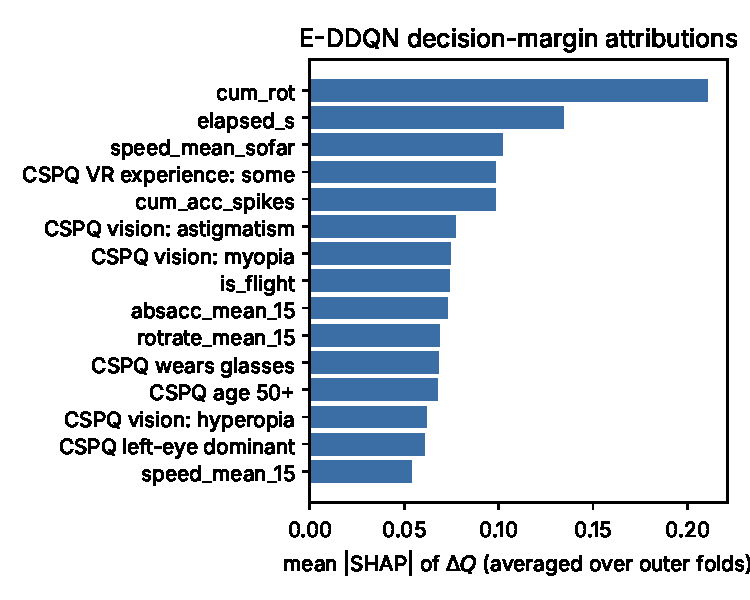
\includegraphics[width=0.92\columnwidth]{figs/shap_margin.pdf}
\caption{Mean absolute SHAP value of the E-DDQN decision margin $\Delta Q$, averaged over the five outer folds (one model per fold; attributions on that fold's test groups).}
\label{fig:shap}
\end{figure}

\section{Discussion}
\label{sec:discussion}

\subsection{Answers to the Research Questions}
\emph{Evaluation protocol.} On these data the split protocol, not the model, decides whether scores look near-perfect: random row-level splits---with or without oversampling---give ROC-AUC above 0.99 because adjacent seconds of a session are near-duplicates with the same label, whereas session-grouped evaluation of the same columns gives \LeakGrpRocAuc. This is a known pitfall rather than a new finding, but it means that accuracy figures on gameplay cybersickness data should be read together with the split protocol.
\emph{RQ1.} On logged data the asymmetric reward encodes a cost-sensitive operating point: the greedy policy is the Bayes rule $P(y=1\mid s)\ge1/6$ of 5:1 cost-sensitive classification, and bootstrapping cannot improve it (Section~\ref{sec:formulation}).
\emph{RQ2.} Under leakage-controlled evaluation with the same search procedure and decision rules, E-DDQN does not outperform the standard DQN, has a higher cost than a cost-weighted random forest in every outer fold (significant under the group bootstrap, but not after Holm adjustment under the more conservative exact sign-flip test), and ranks seconds worse than elapsed time alone, which no model outperformed significantly; no model meets a safety-prioritized target.
\emph{RQ3.} As a sanity check, bounded manipulation of the telemetry channels barely changes threshold-free ranking, which is not evidence of robustness (Section~\ref{sec:attack}), while an adaptive adversary with label knowledge can still lower recall at fixed thresholds by \AttEvasionDropMin--\AttEvasionDropMax{} percentage points.

\subsection{Is E-DDQN Reinforcement Learning?}
With logged data the alarm cannot influence the subsequent telemetry, so the decision problem is a contextual bandit. E-DDQN remains a valid value-based learner of a cost-sensitive detection policy, but (i) the asymmetric reward is mathematically equivalent to a 5:1 cost-sensitive Bayes threshold, so it is a statement about the operating point rather than a different learning objective; (ii) bootstrapping cannot improve the optimal policy, and empirically removing it with E-DDQN's configuration held fixed changed little, whereas E-DDQN's under-performance is more consistent with noisy validation-based selection of configurations that use the questionnaire answers (Section~\ref{sec:why}); and (iii) under bandit feedback the agent observes the reward of one action only, although labels reveal both, which is why full-information replay is the principled way to use the labels. The same reasoning applies to any DQN-based classifier trained on a fixed dataset whose episodes end only with the data: its benefit has to come from estimation effects, and it should be compared with cost-weighted supervised models at the same operating point. Formulations that end an episode when a minority-class sample is misclassified~\cite{lin2020imbalanced,yang2024drlimbalanced} are action-dependent, but the termination acts only as an additional, $\gamma$-dependent penalty on that error (Section~\ref{sec:formulation}), so the same comparison is needed to show that they add more than a different operating point. Adaptive sequential control would require an intervention in the loop---for example an alarm that triggers a rendering mitigation whose effect on later telemetry and symptoms is measured---which no public cybersickness dataset provides.

\subsection{The Safety Objective}
A 5:1 cost makes an alarm the cheaper decision whenever $P(y=1\mid s)\ge1/6$. With a prevalence of 0.44 and weakly informative inputs, almost every second satisfies this, so the cost-optimal policy of every model is close to ``always alarm'': recall is high, but \DOneFPRMin--\DOneFPRMax\,\% of non-event seconds also trigger an alarm. High recall alone is therefore not evidence of a useful safety monitor. Judged on cost, specificity at matched recall, threshold-free ranking and cost curves across ratios, the intended safety objective---near-complete detection with a controlled false-alarm rate---is not achieved by any model on these data. The exposure-time baselines suggest where the obstacle lies: once sessions and linkage groups are not shared between training and test, no model extracted significantly more signal from game telemetry than how long the session has lasted, which distinguishes individual susceptibility only coarsely.

\subsection{The Adversarial Threat Model}
Rendering manipulations that induce sickness are documented~\cite{odeleye2021framerate,tseng2022dark}, and optimization-based input attacks can disable deep cybersickness detectors~\cite{kundu2025securing,ahmed2025adversarialvr}. UFFCSData, however, contains no manipulated sessions, so its label marks cybersickness, not an attack. Our stress tests therefore answer a narrower question than the cited attack studies: how far bounded, physically motivated changes of the logged frame-rate, orientation and locomotion channels move the detectors' decisions. The small effect on ranking is not evidence of a robust design: it reflects the inputs that the selected configurations use and the fact that a perturbation applied to every test session alike can shift scores without reordering them, while at fixed thresholds an adaptive adversary still changes decisions. A detector that used the telemetry more would also be easier to manipulate through it. Demonstrating detection of real rendering attacks requires data in which manipulations are applied to participants under ethical approval and their physiological effects are measured.

\subsection{Limitations}
\label{sec:limits}
(i) A single public dataset with \nSessionsEval{} curated sessions, \nGroupsEval{} independent groups and \nEventSessions{} onsets; confidence intervals are wide, fold-to-fold variation is large, and inference with so few clusters is approximate: the group bootstrap and the exact sign-flip test agree in direction but differ in strength (E-DDQN vs.\ random forest, Holm-adjusted $p=$\,\PHHolmRF{} vs.\ \PHSfRFHolm). (ii) Participant identity cannot be verified; linkage groups are conservative but cannot exclude a participant who answered the questionnaire differently in non-consecutive sessions, and they may merge different people with identical profiles. (iii) The label is a coarse self-report, logged at 1\,Hz but changing rarely within a session, whose elicitation procedure (prompted or spontaneous reports) is not documented, and the binary threshold (discomfort $\ge1$) merges slight with severe discomfort; a safety monitor might target grades 2--3 only, which occur in just \PHGradeFlightSevere{} Flight samples. (iv) The exposure-time baselines, the Holm adjustment, the grouping sensitivity analyses and the cost curves were specified after the primary results were known; they were committed before being run and use the same protocol, but they are post hoc. The within-fold ROC-AUC, the sign-flip tests and the feature-set analysis were added after a pre-submission review, when all other results were known. (v) Perturbations are synthetic and feature-space, their physiological effect is unknown, and the adversary is weaker than optimization-based attacks. (vi) Hyper-parameter search used a modest budget (\HPOBudget{} configurations per family; 12 for logistic regression) that covers a much smaller fraction of the RL search spaces (about \PHSpaceEDDQNMillion{} million configurations for E-DDQN) than of the random-forest space (\PHSpaceRF); a larger budget could change the ranking of the neural models, although the selection-optimism analysis suggests that additional search with the same noisy criterion would mostly increase optimism. (vii) The October-2019 sessions were used only for development and could not serve as an external test set because their camera-orientation channels are constant within every session (a logging defect). (viii) The diagnosis of E-DDQN's under-performance (Section~\ref{sec:why}) is exploratory: feature sets and discount factors were selected, not assigned, so no analysis isolates a cause.

\subsection{Implications}
For cybersickness detection from session data, results should be reported with participant- or session-grouped splits, alongside trivial policies and an exposure-time baseline, because here no model significantly outperformed elapsed time alone. For safety-prioritized detection, an asymmetric reward should be treated as what it is---a cost-sensitive operating point---and RL detectors should be compared with cost-weighted supervised models at matched recall or cost. Claims of robustness to manipulation should state which inputs the detector actually uses and evaluate decisions at fixed thresholds, since an unchanged ranking is not protection. Under grouped evaluation, participant-profile features deserve particular care, because with few groups they can fit group-level label rates that do not transfer.

\section{Conclusion}
\label{sec:conclusion}
We asked whether an asymmetric-reward dueling Double DQN (E-DDQN) improves safety-prioritized cybersickness detection in VR. On the public UFFCSData gameplay dataset the answer is no. On logged data the detection problem is a contextual bandit, and the 5:1 asymmetric reward induces exactly the Bayes threshold of 5:1 cost-sensitive classification. Under a nested, session-grouped protocol fixed before testing, E-DDQN reached a mean cost over seeds of \EDDQNCostCostMean{} and ROC-AUC \EDDQNCostRocAucMean, did not outperform a standard DQN (cost \DQNCostCostMean, ROC-AUC \DQNCostRocAucMean) and had a higher cost than a cost-weighted random forest in every outer fold, marginally in one (cost \RFCostCostMean, ROC-AUC \RFCostRocAucMean; seed ensembles \PHEnsEDDQNCost{} vs.\ \PHEnsRFCost; Holm-adjusted $p=$\,\PHHolmRF{} by group bootstrap and \PHSfRFHolm{} by the more conservative exact sign-flip test). A re-tuning with two further random search draws, specified before it was run, found no draw in which E-DDQN had a significantly lower cost than the standard DQN, and each agent ranked seconds better in one draw; it also showed that E-DDQN's weak primary result reflects its search draw: across draws its within-fold ROC-AUC ranged from \SDEDDQNWfMin{} to \SDEDDQNWfMax{} and its cost from \SDEDDQNCostMin{} to \SDEDDQNCostMax, still above the random forest's as a point estimate. A post-hoc logistic regression on elapsed time alone reached ROC-AUC \PHTimeLRRocAucMean, no primary model ranked seconds significantly better, and no model combined high recall with a controlled false-alarm rate or was shown to improve on always alarming at the 5:1 ratio. Session grouping was essential to these conclusions: splits that share sessions between training and test give near-perfect scores on these data, whereas session-grouped evaluation of the same features gives ROC-AUC \LeakGrpRocAuc. Bounded telemetry perturbations changed ROC-AUC by at most \AttAucMaxAbsChange, which is not evidence of robustness: most selected configurations use exposure-type inputs, and an adaptive adversary still changed decisions at fixed thresholds. Progress on this problem is likely to require datasets with physiological or eye-tracking signals, verified participant identifiers and, for adversarial claims, manipulations applied to participants with measured effects, and evaluations that include grouped splits, trivial and exposure-time baselines, cost-weighted comparators and more than one random search draw per model.


\section*{Data and Code Availability}
The data are the publicly available UFFCSData release~\cite{porcino2019uffcsdata} (AGPL-3.0). All code, the evaluation protocol (\texttt{configs/\allowbreak protocol.json}, committed before any model was trained on the evaluation sessions), the specification of the post-hoc analyses (\texttt{configs/\allowbreak posthoc.json}, committed before those analyses were run), the split tables, the per-sample predictions of every model and the scripts that produce every number, table and figure of this paper are archived at [DOI to be added on deposit]. A single script regenerates everything from the raw XML files. Seeds are fixed for data splitting (20261012), hyper-parameter search (777; 801--802 for the post-hoc baselines) and final training (1000--1004); CPU execution with one thread per process was used, and minor floating-point differences across hardware are possible.

\section*{Acknowledgment}
The authors thank Universiti Teknologi PETRONAS for institutional and computational support, and the authors of the UFFCSData dataset for making their data public.

\section*{Conflict of Interest}
The authors declare no conflict of interest.

\section*{Funding}
This research received no specific grant from any funding agency in the public, commercial, or not-for-profit sectors.

\bibliographystyle{IEEEtran}
\bibliography{refs}

\end{document}
